\documentclass{article}
\usepackage{amsmath,amssymb,amstext,mathtools,array,url,bm,graphicx,color,epsfig}
\usepackage{fullpage,setspace}
\usepackage{authblk}
\usepackage{filecontents}
\usepackage{natbib}
\usepackage{lineno}
\usepackage[colorlinks]{hyperref}
\usepackage{subcaption}
\usepackage{float}
\usepackage[flushleft]{threeparttable}

\def\dt{\partial t}
\def\dx{\partial x}
\def\dy{\partial y}

\def\dz{\partial z}
\def\BE{\begin{equation}}
\def\EE{\end{equation}}
\def\half{\frac{1}{2}}
\def\calT{\cal T}
\def\Deltax{\Delta x}
\def\Deltat{\Delta t}
\DeclareSymbolFont{largesymbolsA}{U}{txexa}{m}{n}
\DeclareMathSymbol{\varprod}{\mathop}{largesymbolsA}{16}

\newtheorem{theorem}{Theorem}
\newtheorem{acknowledgement}[theorem]{Acknowledgement}
\newtheorem{algorithm}[theorem]{Algorithm}
\newtheorem{axiom}[theorem]{Axiom}
\newtheorem{case}[theorem]{Case}
\newtheorem{claim}[theorem]{Claim}
\newtheorem{conclusion}[theorem]{Conclusion}
\newtheorem{condition}[theorem]{Condition}
\newtheorem{conjecture}[theorem]{Conjecture}
\newtheorem{corollary}[theorem]{Corollary}
\newtheorem{criterion}[theorem]{Criterion}
\newtheorem{definition}[theorem]{Definition}
\newtheorem{example}[theorem]{Example}
\newtheorem{exercise}[theorem]{Exercise}
\newtheorem{lemma}[theorem]{Lemma}
\newtheorem{notation}[theorem]{Notation}
\newtheorem{problem}[theorem]{Problem}
\newtheorem{proposition}[theorem]{Proposition}
\newtheorem{remark}[theorem]{Remark}
\newtheorem{solution}[theorem]{Solution}
\newtheorem{summary}[theorem]{Summary}
\newenvironment{proof}[1][Proof]{\noindent\textbf{#1.} }{\ $\square$}


\begin{document}

\title{\bf Comparative anatomy of geophysical flow models and modeling assumptions using uncertainty quantification}
\author[1,3]{Abani K. Patra}
\author[2]{Andrea Bevilacqua}
\author[1]{Ali Akhavan-Safaei}
\author[4]{E. Bruce Pitman}
\author[2]{Marcus I. Bursik}
\author[2]{David Hyman}

\affil[1]{\textit{Dept. of Mech. and  Aero. Eng., University at Buffalo, Buffalo NY 14260} }
\affil[2]{\textit{Dept. of Geology, University at Buffalo, Buffalo NY 14260} }
\affil[3]{\textit{Comp. Data Science and Eng., University at Buffalo, Buffalo NY 14260} }
\affil[4]{\textit{Dept. of Materials Design and Innovation, University at Buffalo, NY, 14260}}

\date{\texttt{\{abani,abevilac,aliakhav,pitman,mib,davidhym\}@buffalo.edu}}


\maketitle
\tableofcontents

\abstract
We develop a new statistically driven method for analyzing the modeling of geophysical flows, in presence of many models advocated by different modelers and incorporating different modeling assumptions. Limited and sparse data on the modeled phenomena usually does not permit a clean discrimination among models for fitness of purpose, and, heuristic choices are usually made, especially for critical predictions of behavior that has not been experienced. We advocate here for characterizing models and the modeling assumptions they represent using a statistical approach over the full range of applicability of the models. Such a characterization may then be used to decide the appropriateness of a model for use, and, perhaps as needed weighted compositions of models for better predictive power. We present our method comparing three different models arising from different rheology assumptions, and the data show unambiguously the performance of the models across a wide range of possible flow regimes and topographies. The analysis of latent variables in the models is particularly illustrative of the impact of modeling assumptions. Knowledge of which assumptions dominate, and, by how much, is achieved in two different case studies: a small scale inclined plane with a flat runway, and the large scale topography on the SW lope of Volc\'{a}n de Colima (MX).



\newpage
\section{Introduction}
This paper presents a systematic approach to the study of models of complex systems, applied to the case of geophysical mass flows modeling.

A simple though not necessarily comprehensive definition of a model is that: \begin{quote}{\it A model is a representation of a postulated relationship among inputs and outputs of a system, usually, informed by observation and a hypothesis that best explains the relationship.}\end{quote} The definition captures two of the most important characteristics
\begin{itemize}
\item models depend on a {\it hypothesis}, and,
\item models use the {\it data from observation} to validate and refine the hypothesis.
\end{itemize}
Errors and uncertainty in the data and limitations in the hypothesis (usually a tractable and computable mathematical construct articulating beliefs like proportionality, linearity etc.) are immediate challenges that must be overcome to construct useful and credible models.

A model is most useful in predicting the behavior of a system for unobserved inputs, and, interpreting or explaining of the system's behavior. Since, models require a hypotheses, it follows  that the model is a formulation of a belief about the data. The immediate consequence of this is that the model may be very poor about such prediction, since, the {\it subjectivity of the belief} can never be completely eliminated \citep{Kennedy2001, Higdon2004} even when sufficient care is taken to use all the available data and information. Secondly, the data at hand may not provide enough information about the system to characterize its behavior at the desired prediction. This {\it data inadequacy} is rarely characterized even for verified and validated models and codes. What makes this problem even more acute is that we are often interested in modeling outcomes that are not observed and often not observable.

The consequence of this lack of knowledge and limited data is the multiplicity of beliefs about the complex system being modeled and a profusion of models based on different modeling assumptions and data use. These competing models lead to much debate among scientists. Principles like ``Occam's razor" and Bayesian statistics \cite{Farrell2015} provide some guidance but simple robust approaches that allow the testing of models for fitness need to be developed. We present in this paper a simple data driven approach to discriminate among models and the modeling assumptions implicit in each model, given a range of phenomena to be studied. We illustrate the approach by work on geophysical mass flows.

\subsection{Models and assumptions}
An assumption is a simple concept -- any atomic postulate about relationships among quantities under study. Models are compositions of many such assumptions. The study of models is, thus, implicitly a study of these assumptions and their composability and applicability in a particular context. Sometimes a good model contains a useless assumption that may be removed, sometimes a good assumption could be added to a different model - these are usually subjective choices, not data driven. Moreover, the correct assumptions may change through time, making {\em model choice} more difficult.

The rest of the paper will define our approach and a simple illustration using three models for large scale mass flows incorporated in our large scale mass flow simulation framework  TITAN2D \citep{Patra2005,Patra2006, Yu2009, Aghakhani2016}. The $\mathrm{4^{\mathrm{th}}}$ release of TITAN2D offers multiple rheology options in the same cyber-infrastructure. The availability of three distinct models for similar phenomena in the same tool provides us the  ability to directly compare inputs, outputs and internal variables in all the three models.

So far, TITAN2D has been successfully applied to the simulation of different geophysical mass flows with specific characteristics \citep{Sheridan2005, Rupp2006, Norini2008, Charbonnier2009, Procter2010, Sheridan2010, Sulpizio2010, Capra2011}. Several studies involving TITAN2D were recently directed towards a statistical study of geophysical flows, focusing on uncertainty quantification \citep{Dalbey2008, Dalbey2009, Stefanescu2012b, Stefanescu2012a}, or on the more efficient production of hazard maps \citep{Bayarri2009, Spiller2014,Bayarri2015, Ogburn2016}.

\subsection{Analysis of modeling assumptions and models }
Let us define $\left(M(A), P_{M(A)}\right)$, where $A$ is a set of assumptions, $M(A)$ is the model which combines those assumptions, and $P_M$ is a probability distribution in the parameter space of $M$. For the sake of simplicity we assume $P_M$ to be uniformly distributed on selected parameter ranges. While the support of $P_M$ can be restricted to a single value by solving an inverse problem for the optimal reconstruction of a particular flow, this is not possible if we are interested in the general predictive capabilities of the model, where we are interested in the outcomes over a whole range.

\paragraph{Stage 1: Parameter Ranges} In this study, we always assume:
$$P_M\sim \bigotimes_{i=1}^{N_M} Unif(a_{i,M},b_{i,M}),$$
where $N_M$ is the number of parameters of $M$. These parameter ranges will be chosen using information gathered from the literature about the physical meaning of those values together with a preliminary testing for physical consistency of model outcomes and range of inputs/outcomes of interest. If the total friction of the models does not cover a similar span, the statistical comparison is dominated by trivial macroscopic differences, and cannot focus on the rheology details.

\paragraph{Stage 2 Simulations and Data Gathering}
The simulation algorithms can be represented as:
\begin{figure}[H]
\centerline{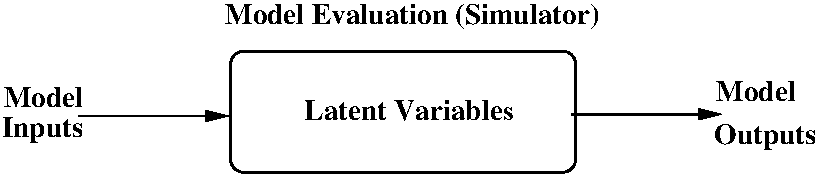
\includegraphics[width=0.85\textwidth]{modelproc.pdf}}
\centering
\caption{Models and variables}
\end{figure}

The \emph{model inputs} are the parameters of $M$, the \emph{latent variables} include quantities in the model evaluation that are ascribable to specific assumptions $A_i$. These are usually not observed as outputs from the model. For example in momentum balances of complex flow calculations these could be values of different source terms, dissipation terms and inertia terms. Finally, the \emph{model outputs} include explicit outcomes e.g., for flow calculations these could be flow height, lateral extent, area, velocity, acceleration, and derived quantities such as Froude number $Fr$. In general, for each quantity of interest (QoI), we use a Monte Carlo simulation, sampling the input variables and obtaining a family of graphs plotting their expectation, and their 5$^{\mathrm{th}}$ and 95$^{\mathrm{th}}$ percentiles. Our sampling technique of the input variables is based on the Latin Hypercube Sampling (LHS) idea, and in particular, on the improved space-filling properties of the orthogonal array-based Latin Hypercubes (see Appendix A).

\paragraph{Stage 3 Results Analysis} These and other statistics can now be compared to determine the need for different modeling assumptions and the relative merits of different models. Thus, analysis of the data gathered over the entire range of flows for the state variables and outcomes leads to a quantitative basis for accepting or rejecting particular assumptions or models for specific outcomes.

\section{Modeling of geophysical mass flows}\label{subsec:FlowTypes}
Dense large scale granular avalanches are a complex class of flows with physics that has often been poorly captured by models that are computationally tractable. Sparsity of actual flow data (usually only a posteriori deposit information is available), and large uncertainty in the mechanisms of initiation and flow propagation, make the modeling task challenging, and a subject of much continuing interest. Models that appear to represent the physics well in certain flows, may turn out to be poorly behaved in others, due to intrinsic physical, mathematical or numerical issues. Nevertheless, given the large implications on life and property, many models with different modeling assumptions have been proposed. For example in \cite{Iverson1997, Iverson2001, Denlinger2001, Pitman2003a, Denlinger2004, Iverson2004}, the depth-averaged model was applied in the simulation of test geophysical flows in large scale experiments. Several studies were specifically devoted to the modeling of volcanic mass flows \citep{Bursik2005,Kelfoun2005,Charbonnier2009,Kelfoun2009,Procter2010,Kelfoun2011,Charbonnier2013}. In fact, volcanoes are great sources for a rich variety of geophysical flow types and provide field data from past flow events.

Modeling in this case proceeds by first assuming that the laws of mass and momentum conservation hold for properly defined system boundaries. The scale of these flows -- very long and wide with small depth led to the first most generally accepted assumption -- shallowness \cite{SavageHutter1989}. This allows an integration through the depth to obtain simpler and more computationally tractable equations. This is the next of many assumptions that have to be made. Both of these are fundamental assumptions which can be tested in the procedure we established above. Since, there is a general consensus and much evidence in the literature of the validity of these assumptions we defer analysis of these to future work.

The depth-averaged Saint-Venant equations that result are:
\begin{eqnarray}
\label{eq:D_A}
\frac{\partial h}{\partial t} +
\frac{\partial}{\partial x}(h \bar{u}) +
\frac{\partial}{\partial y}(h\bar{v}) &=& 0 \nonumber \\
\frac{\partial}{\partial t} (h\bar{u}) +
\frac{\partial}{\partial x}\left(h\bar{u}^2 + \frac{1}{2}k g_{z}h^2\right) + \frac{\partial}{\partial y}(h\bar{u}\bar{v}) &=& S_{x}\\
\frac{\partial}{\partial t} (h\bar{v}) +
\frac{\partial}{\partial x}(h\bar{u}\bar{v}) +
\frac{\partial}{\partial y}\left(h\bar{v}^2 + \frac{1}{2}k g_{z}h^2\right) &=& S_{y} \nonumber
\end{eqnarray}
Here the Cartesian coordinate system is aligned such that $z$ is normal to the surface; $h$ is the flow height in the $z$ direction; $h\bar{u}$ and $h\bar{v}$ are respectively the components of momentum in the $x$ and $y$ directions; and $k$ is the coefficient which relates the lateral stress components, $\bar{\sigma}_{xx}$ and $\bar{\sigma}_{yy}$, to the normal stress component, $\bar{\sigma}_{zz}$. The definition of this coefficient depends on the constitutive model of the flowing material we choose. Note that $\frac{1}{2} k g_z h^2$ is the contribution of hydrostatic pressure to the momentum fluxes. $S_x$ and $S_y$ are the sum local stresses: they include the gravitational driving forces, the basal friction force resisting to the motion of the material, and additional forces specific of rheology assumptions.

The final class of assumptions are the assumptions on the rheology of the flows -- in particular in this context assumptions used to model different dissipation mechanisms embedded in $S_x, S_y$ that lead to a plethora of models with much controversy on the most suitable model.

\subsection{Overview of the models}\label{subsec:Models}
In the three following sections, we briefly describe \emph{Mohr-Coulomb} (MC), \emph{Pouliquen-Forterre} (PF) and \emph{Voellmy-Salm} (VS) models. Models based on additional heterogeneous assumptions are possible, either more complex \citep{PitmanLe2005,Iverson2014} or more simple \citep{DadeHuppert1998}, but we decided to focus on these three because of their historical relevance and their comparable degree of complexity.

\subsubsection{Mohr-Coulomb}\label{MCM}
Based on the long history of studies in soil mechanics \citep{Rankine1857,Jaeger1989}, the Mohr-Coulomb rheology (MC) was developed and used to represent the behavior of geophysical mass flows \cite{SavageHutter1989}.

Shear and normal stress are assumed to obey Coulomb friction equation, both within the flow and at its boundaries. In other words,
\begin{equation}
\tau = \sigma \tan \phi,
\end{equation}
where $\tau$ and $\sigma$ are respectively the shear and normal stresses on failure surfaces, and $\phi$ is a friction angle. This relationship does not depend on the flow speed.

We can summarize the MC rheology assumptions as:
\begin{itemize}
\item \textit{Basal Friction} based on a constant friction angle.

\item \textit{Internal Friction} based on a constant friction angle.

\item \textit{Earth pressure coefficient} formula depends on the Mohr circle.

\item Velocity based \textit{curvature effects} are included into the equations.
\end{itemize}

Under the assumption of symmetry of the stress tensor with respect to the \textit{z} axis, the earth pressure coefficient $k=k_{ap}$ can take on only one of three values $\{ 0, \pm 1\}$. The material yield criterion is represented by the two straight lines at angles $\pm \phi$ (the internal friction angle) relative to horizontal direction. Similarly, the normal and shear stress at the bed are represented by the line $\tau=-\sigma \tan(\delta)$ where $\delta$ is the bed friction angle.

\paragraph{MC equations} As a result, we can write down the source terms of the Eqs. (\ref{eq:D_A}):
\begin{eqnarray}\label{S_terms_MC}
S_x =& g_x h  - \frac{\bar{u}}{\| \underset{^\sim}{\bar{\textbf u}} \|} \left[h\left(g_z+\frac{\bar{u}^2}{r_x}\right)\tan(\phi_{bed})\right] - h k_{ap} \ {\rm sgn}\left(\frac{\partial \bar{u}}{\partial y}\right) \frac{\partial (g_z h)}{\partial y} \sin(\phi_{int}) \nonumber \\
 S_y =& g_y h  - \frac{\bar{v}}{\| \underset{^\sim}{\bar{\textbf u}} \|} \left[h\left(g_z +\frac{\bar{v}^2}{r_y}\right)\tan(\phi_{bed})\right] - h k_{ap} \ {\rm sgn}\left({\frac{\partial \bar{v}}{\partial x}}\right) \frac{\partial (g_z h)}{\partial x} \sin(\phi_{int})
\end{eqnarray}
Where, $\underset{^\sim}{\bar{\textbf u}} = (\bar{u} , \bar{v})$, is the depth-averaged velocity vector, $r_x$ and $r_y$ denote the radii of curvature
of the local basal surface. The inverse of the radii of curvature is usually approximated with the partial derivatives of the basal slope, e.g., $1/r_x = \partial \theta_x/\partial x$, where $\theta_x$ is the local bed slope.

In our study, sampled input parameters are $\phi_{bed}$, and $\Delta \phi:=\phi_{int}-\phi_{bed}$. In particular, the range of $\phi_{bed}$ depends on the case study, while $\Delta \phi \in [2^{\mathrm{\circ}}, 10^{\mathrm{\circ}}]$ \citep{Dalbey2008}.

\subsubsection{Pouliquen-Forterre}\label{PFM}
The scaling properties for granular flows down rough inclined planes led to the development of the Pouliquen-Forterre rheology (PF), assuming a variable frictional behavior as a function of Froude Number and flow depth \citep{Pouliquen1999, ForterrePouliquen2002, PouliquenForterre2002, ForterrePouliquen2003}.

PF rheology assumptions can be summarized as:
\begin{itemize}
\item \textit{Basal Friction} is based on an interpolation of two different friction angles, based on the flow regime and depth.

\item \textit{Internal Friction} is neglected.

\item \textit{Earth pressure coefficient} is equal to one.

\item Normal stress is modified by a \textit{hydrostatic pressure force} related to the flow height gradient.

\item Velocity based \textit{curvature effects} are included into the equations.
\end{itemize}

Two critical slope inclination angles are defined as functions of the flow thickness, namely $\phi_{start}(h)$ and $\phi_{stop}(h)$. The function $\phi_{stop}(h)$ gives the slope angle at which a steady uniform flow leaves a deposit of thickness $h$, while $\phi_{start}(h)$ is the angle at which a layer of thickness $h$ is mobilized. They define two different basal friction coefficients.
\begin{eqnarray}
\mu_{start}(h)=\tan(\phi_{start}(h))\\
\mu_{stop}(h)=\tan(\phi_{stop}(h))
\end{eqnarray}

An empirical friction law $\mu_{b}(\|\underset{^\sim}{\bar{\textbf{u}}} \| , h)$ is then defined in the whole range of velocity and thickness. The expression changes depending on two flow regimes, according to a parameter $\beta$ and the Froude number $Fr=\| \underset{^\sim}{\bar{\textbf{u}}} \| / \ \sqrt{h g_{z}}$.

\paragraph{Dynamic friction regime - $Fr \ge \beta$}
\begin{equation}\label{mu_beta1}
\mu(h, Fr)=\mu_{stop}(h \beta / Fr)
\end{equation}

\paragraph{Intermediate friction regime - $0 \le Fr < \beta$}
\begin{equation}\label{mu_beta2}
\mu(h, Fr)=\left(\frac{Fr}{\beta}\right)^\gamma [\mu_{stop}(h)-\mu_{start}(h)] + \mu_{start}(h),
\end{equation}
where $\gamma$ is the power of extrapolation, assumed equal to $10^{-3}$ in the sequel \citep{PouliquenForterre2002}.

The functions $\mu_{stop}$ and $\mu_{start}$ are defined by:
\begin{equation}\label{mu-stop}
\mu_{stop}(h)=\tan\phi_{1} + \frac{\tan\phi_{2}-\tan\phi_{1}}{1+h/\it \mathcal{L}}
\end{equation}
and
\begin{equation}\label{mu-start}
\mu_{start}(h)=\tan\phi_{3} + \frac{\tan\phi_{2}-\tan\phi_{1}}{1+h/\it \mathcal{L}}
\end{equation}
The critical angles $\phi_{1}$, $\phi_{2}$ and $\phi_{3}$ and the parameters $\mathcal{L}, \beta$ are the parameters of the model.

In particular, $\mathcal{L}$ is the characteristic depth of the flow over which a transition between the angles $\phi_{1}$ to $\phi_{2}$ occurs, in the $\mu_{stop}$ formula. In practice, if $h\ll \mathcal L$, then $\mu_{stop}(h)\approx \tan\phi_{2}$, and if $h\gg \mathcal L$, then $\mu_{stop}(h)\approx\tan\phi_{1}$.

\paragraph{PF equations} The depth-averaged Eqs. (\ref{eq:D_A}) source terms thus take the following form:
\begin{eqnarray}\label{eq:S_terms_PF}
S_{x} &=&  g_{x} h -  \frac{\bar{u}}{\| \underset{^\sim}{\bar{\textbf{u}}} \|}\left[h \left(g_z+\frac{\bar{u}^2}{r_x}\right) \ \mu_{b}(\|\underset{^\sim}{\bar{\textbf{u}}} \| , h)\right] \ + g_{z}h\frac{\partial h}{\partial x} \nonumber \\
S_{y} &=&  g_{y} h - \frac{\bar{v}}{\| \underset{^\sim}{\bar{\textbf{u}}} \|}\left[h \left(g_z +\frac{\bar{v}^2}{r_y}\right) \ \mu_{b}(\|\underset{^\sim}{\bar{\textbf{u}}} \| , h)\right] \ + g_{z}h\frac{\partial h}{\partial y}
\end{eqnarray}

In our study, sampled input parameters are $\phi_1$, $\Delta \phi_{12}:=\phi_2-\phi_1$, and $\beta$. In particular, the range of $\phi_1$ depends on the case study, whereas $\Delta \phi_{12} \in [10^{\mathrm{\circ}}, 15^{\mathrm{\circ}}]$, and $\beta \in [0.1, 0.85]$. Moreover, $\phi_3=\phi_1+1^\mathrm{\circ}$, and $\mathcal{L}$ is equal to $1 dm$ and $1 mm$ in the two case studies, respectively \citep{PouliquenForterre2002,ForterrePouliquen2003}.

\subsubsection{Voellmy-Salm}\label{VSM}
The theoretical analysis of dense snow avalanches led to the VS rheology (VS) \citep{Voellmy1955, Salm1990, Salm1993, Bartelt1999}. Dense snow or debris avalanches consist of mobilized, rapidly flowing ice-snow mixed to debris-rock granules \citep{BarteltMcArdell2009}. The VS rheology assumes a velocity dependent resisting term in addition to the traditional basal friction, ideally capable of including an approximation of the turbulence-generated dissipation. Many experimental and theoretical studies were developed in this framework \citep{Gruber2007, Kern2009, Christen2010, Fischer2012}.

The following relation between shear and normal stresses holds:
\begin{equation}
\tau = \mu \sigma + \frac{\rho \| \underline{\textbf g} \|}{\xi} \| \underset{^\sim}{\bar{\textbf u}} \|^2,
\end{equation}
where, $\sigma$ denotes the normal stress at the bottom of the fluid layer and $\underline{\textbf g} = (g_{x} , g_{y} , g_{z})$ represents the gravity vector. The two parameters of the model are the bed friction coefficient $\mu$ and the velocity dependent friction coefficient $\xi$.

We can summarize VS rheology assumptions as:
\begin{itemize}
\item \textit{Basal Friction} is based on a constant coefficient, similarly to the MC rheology.

\item \textit{Internal Friction} is neglected.

\item \textit{Earth pressure coefficient} is equal to one.

\item Additional \textit{turbulent friction} is based on the local velocity by a quadratic expression.

\item Velocity based \textit{curvature effects} are included into the equations, following an alternative formulation.
\end{itemize}

The effect of the topographic local curvatures is addressed with terms containing the local radii of curvature $r_x$ and $r_y$. In this case the expression is based on the speed instead of the scalar components of velocity \cite{PudasainiHutter2003,Fischer2012}.

\paragraph{VS equations} Therefore, the final source terms take the following form:
\begin{eqnarray}
\label{eq:S_terms_VS}
S_{x} &=&  g_{x} h - \frac{\bar{u}}{\| \underset{^\sim}{\bar{\textbf u}}\|} \ \left[ h \left(g_{z} + \frac{\| \underset{^\sim}{\bar{\textbf u}} \|^2}{r_{x}} \right)\mu+ \frac{\| \underset{^\sim}{\textbf g} \|}{\xi}\| \underset{^\sim}{\bar{\textbf u}} \|^2\right], \nonumber \\
S_{y} &=& g_{y} h - \frac{\bar{v}}{\| \underset{^\sim}{\bar{\textbf u}}\|} \ \left[ h \left(g_{z} + \frac{\| \underset{^\sim}{\bar{\textbf u}} \|^2}{r_{y}} \right)\mu+ \frac{\| \underset{^\sim}{\textbf g} \|}{\xi}\| \underset{^\sim}{\bar{\textbf u}} \|^2\right].
\end{eqnarray}

In our study, sampled input parameters are $\mu$, and $\xi$, on ranges depending on the case study. In particular, $\xi$ uniform sampling is accomplished in log-scale. In fact, values of $\xi$ between 250 and 4,000 $m/s^2$ have been described for snow avalanches \citep{Salm1993,Bartelt1999,Gruber2007}.

\subsection{Latent variables}\label{sec:Fterms}
For analysis of modeling assumptions we need to record and classify the results of different modeling assumptions. In our case study, we focus on the right-hand side terms in the momentum equation, and we call them RHS forces or latent variables since they are internal to the computation and rarely visible as a system output.
\begin{align}
\boldsymbol{RHS_1} = [g_x h,g_y h],
\end{align}
it is the gravitational force term, it has the same formulation in all models.

The expression of {\bf basal friction force} $\boldsymbol{RHS_2}$ depends on the model:
\begin{align}
\boldsymbol{RHS_2} =& -h g_z\tan(\phi_{bed})\left[\frac{\bar{u}}{\| \underset{^\sim}{\bar{\textbf u}} \|}, \frac{\bar{v}}{\| \underset{^\sim}{\bar{\textbf u}} \|} \right],\textmd{ in MC model.}\nonumber\\
\boldsymbol{RHS_2} =& - h g_z \ \mu_{b}(\|\underset{^\sim}{\bar{\textbf{u}}} \| , h)\left[\frac{\bar{u}}{\| \underset{^\sim}{\bar{\textbf{u}}} \|}, \frac{\bar{v}}{\| \underset{^\sim}{\bar{\textbf{u}}} \|}\right],\textmd{ in PF model.}\\
\boldsymbol{RHS_2} =& -h g_{z} \mu\left[\frac{\bar{u}}{\| \underset{^\sim}{\bar{\textbf u}}\|} , \frac{\bar{v}}{\| \underset{^\sim}{\bar{\textbf u}}\|}\right],\textmd{ in VS model.}\nonumber
\end{align}

The expression of the force related to the {\bf topography curvature}, $\boldsymbol{RHS_3}$, also depends on the model:
\begin{align}
\boldsymbol{RHS_3} =&-h \tan(\phi_{bed})\left[\frac{\bar{u}^3}{r_x\| \underset{^\sim}{\bar{\textbf{u}}} \|}, \frac{\bar{v}^3}{r_y\| \underset{^\sim}{\bar{\textbf{u}}} \|}\right],\textmd{ in MC model.}\nonumber\\
\boldsymbol{RHS_3} =& -h\ \mu_{b}(\|\underset{^\sim}{\bar{\textbf{u}}} \|,h)\left[\frac{\bar{u}^3}{r_x\| \underset{^\sim}{\bar{\textbf{u}}} \|}, \frac{\bar{v}^3}{r_y\| \underset{^\sim}{\bar{\textbf{u}}} \|}\right],\textmd{ in PF model.}\\
\boldsymbol{RHS_3} =& -h \mu\left[\frac{\bar{u}\| \underset{^\sim}{\bar{\textbf u}} \|}{r_{x}},\frac{\bar{v}\| \underset{^\sim}{\bar{\textbf u}} \|}{r_{y}}\right],\textmd{ in VS model.}\nonumber
\end{align}

All the three models have an additional force term, having a different expressions and different meaning in the three models:
\begin{align}
\boldsymbol{RHS_4} =&  - h k_{ap}\sin(\phi_{int})\left[ \ {\rm sgn}(\frac{\partial \bar{u}}{\partial y}) \frac{\partial (g_z h)}{\partial y},\ {\rm sgn}({\frac{\partial \bar{v}}{\partial x}}) \frac{\partial (g_z h)}{\partial x}\right],\textmd{ in MC model.}\nonumber\\
\boldsymbol{RHS_4} =& g_{z}h\left[\frac{\partial h}{\partial x}, \frac{\partial h}{\partial y}\right],\textmd{ in PF model.}\\
\boldsymbol{RHS_4} =& -\frac{\| \underset{^\sim}{\textbf g} \|}{\xi}\| \underset{^\sim}{\bar{\textbf u}} \|^2\left[\frac{\bar{u}}{\| \underset{^\sim}{\bar{\textbf u}}\|} \ ,\frac{\bar{v}}{\| \underset{^\sim}{\bar{\textbf u}}\|}\right],\textmd{ in VS model.}\nonumber
\end{align}
These latent variables can be analyzed locally and globally for discriminating among the different modeling assumption.

\subsection{Monte Carlo Process and Statistical Analysis}
In our study, the flow range is defined by establishing boundaries for inputs like flow volume V and different rheology coefficients characterizing the models.  Latin Hypercube Sampling is performed over $[0,1]^3$ for the MC and VS input parameters, and $[0,1]^4$ for PF input parameters. Those dimensionless samples are linearly  mapped to fill the required intervals (see Appendix A).

Following the simulations, we generate data for each sample run and each outcome and latent variable $f(\underline{\textbf x},t)$ calculated as a function of time on the elements of the computational grid. This analysis generates tremendous volume of data which must then be analyzed using statistical methods for summative impact. The latent variables in this case are the mass and force terms in the conservation laws defined above. %In more detail, local sampling is performed by considering the elements of the adapting mesh which are found to contain the sample points.

We devise many statistical measures for analyzing the data. For instance, let $(F_i(x,t))_{i=1,\dots, 4}$ be an array of force components, where $x\in \mathbf R^2$ is a spatial location, and $t\in T$ is a time instant. The degree of contribution of those force terms can be significantly variable in space and time, and we define the \emph{dominance factors} $(p_j)_{j=1,\dots, k}$, i.e., the probability of each $F_j$ to be the dominant force at $(x,t)$. Those probabilities provide insight into the dominance of a particular source or dissipation (identified with a particular modeling assumption) term on the model dynamics. The dominance factors can be adopted to define a statistical decomposition of the contributions of the forces, as detailed in Appendix B.

Additionally, spatial integrals are defined by $F(t)=\int_{\mathbb R^k}f(\underline{\textbf x},t) d\underline{\textbf x}$. In the most of the cases $k=2$, and $d\underline{\textbf x}$ is given by the area of the mesh elements except for speed $k=3$, and $d\underline{\textbf x}$ is the element of volume corresponding to the mesh elements {\bf ****unclear}.


Force contributions represent an additional tool to compare the different force terms, following a less restrictive approach than the Dominance Factors. They are obtained dividing the force terms described in section \ref{sec:Fterms} by the dominant force $\Phi$.

In general we focus on the moduli of the forces, or their projection on the slope direction. Hence, in the following the forces are scalar and not vectorial terms. It is important to remark that all the forces depend on the input variables, and they are thus considered as random variables. The definitions are not depending on the location, but all the results will significantly depend of that choice. Next notation will assume to be in a selected location $x=L_k$, where $k\ge 1$.

\begin{definition}[Contribution coefficients]
Let $(F_i)_{i\in I}$ be random variables on $(\Omega, \mathcal F, P)$, representing the considered force components in location $x$ at time $t$. Then, for each component $i$, the contribution coefficient is defined as:
$$C_i:=\mathbb E\left[\frac{F_i}{\Phi}\right],$$
where $\Phi$ is a dominating function, i.e. $\Phi\ge |F_i|$, $\forall i\in I$.
\end{definition}
The \emph{total force}, i.e $\sum_i F_i$ excluding the inertial terms, is not a good candidate for a dominating function. Indeed, the terms often have opposite signs, and their sum can be really small. Another issue is given by the existence of a subset of times $\Theta$ characterized by the absence of flow in the selected location $x$. In $\Theta$ the dominant force is null, and cannot be the denominator of a fraction.

In our study $\Phi$ is the dominant force - our approach is based on the $l^\infty$ norm:
$$\Phi:=\left\{
    \begin{array}{ll}
      \max_i |F_i|, & \hbox{if not null;} \\
      1, & \hbox{otherwise.}
    \end{array}
  \right.$$
In particular, for a particular location $x$, time $t$, and parameter sample $\omega$, we have $C_i=0$ if there is no flow or all the forces are null. The expectation of $C_i$ is reduced by the chance of $F_i$ being small compared to the other terms, or by the chance of having no flow in $(x,t)$. Moreover, $\mathbb E[C_i]\in[-1,1]$, $\forall i$.



\section{Small scale flow on inclined plane and flat runway}\label{sec:QoIs}
Our first case study assumes very simple boundary conditions, and corresponds to a laboratory experiment fully described in \cite{Webb2004, Bursik2005, WebbBursik2016}. It is a classical flow down an inclined plane set-up, including a change in slope to an horizontal plane (Fig. \ref{fig:Ramp-first}). Modeling flow of granular material down an inclined plane was explored in detail by several studies, both theoretically and experimentally (e.g. \cite{RuyerQuil2000, Silbert2001, Pitman2003b}).

In our setting, four locations are selected among the center line of the flow to accomplish local testing. These are: the initial pile location $L_1=(-0.7,0)$ m, the middle of the inclined plane $L_2=(-0.35,0)$ m, the change in slope $L_3=(0,0)$ m, the middle of the flat runway $L_4=(0.15,0)$ m.
\begin{figure}[H]
    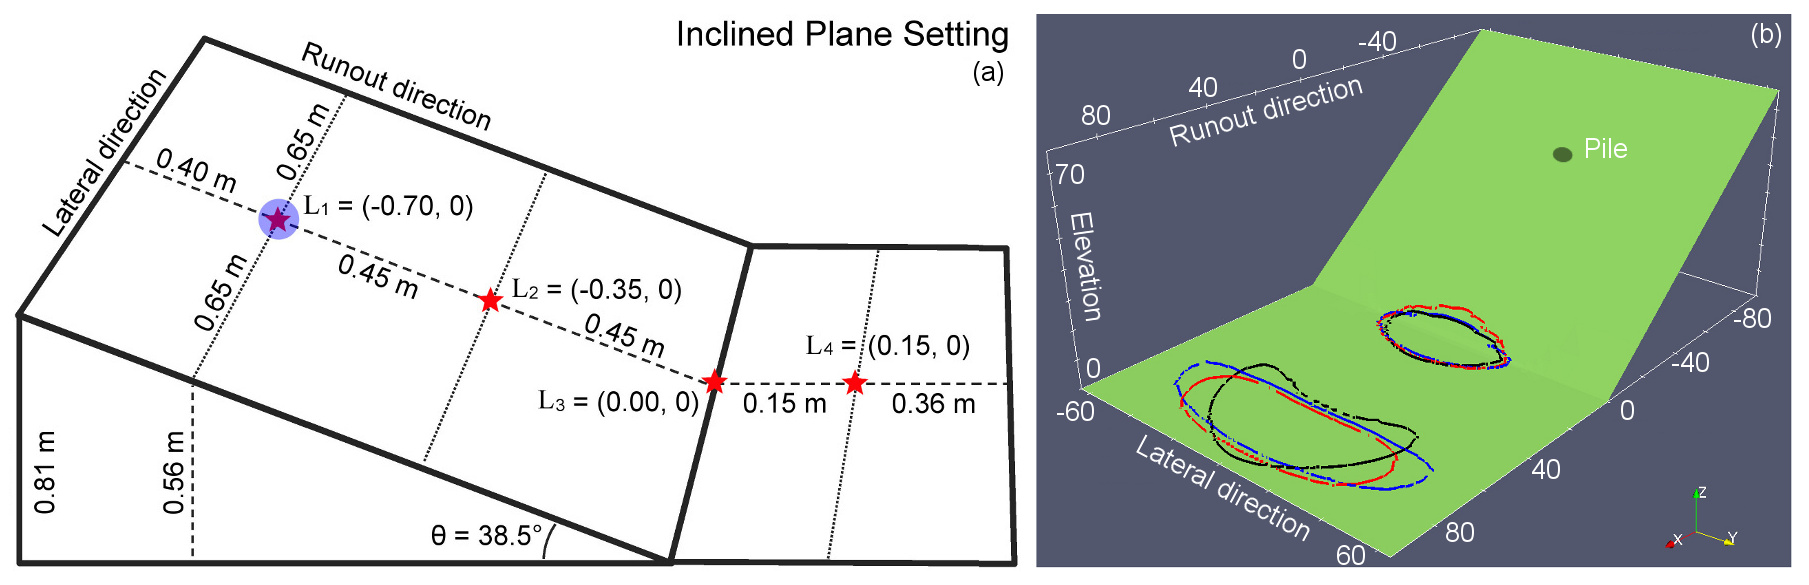
\includegraphics[width=1\textwidth]{InclinedPlane/InclPlane_new.jpg}
    \centering
    \caption{(a) Inclined plane overview, including local samples sites (red stars). Pile location is marked by a blue dot. (b) Contours of $h = 1.0$ mm at last simulated snapshot ($t = 1.5$ sec) for simulated flows with \emph{minimum runout} obtained from \emph{\textbf{min. volume -- max. resistance}}, and \emph{maximum runout} obtained from \emph{\textbf{max. volume -- min. resistance}}. {\color{red} \textbf{---}} : MC, {\color{blue} \textbf{---}} : PF, \textbf{---} : VS.} \label{fig:Ramp-first}
\end{figure}

\subsection{Preliminary consistency testing of the input ranges}\label{consistency}
Addressing a similar case study \cite{Dalbey2008} assumed $\phi_{bed}=[15^\mathrm{\circ}, 30^\mathrm{\circ}]$, while \cite{WebbBursik2016} performed a series of laboratory experiments and found $\phi_{bed}=[18.2^\mathrm{\circ}, 34.4^\mathrm{\circ}]$. We relied on those published parameter choices to select a comprehensive parameter range. Figure \ref{fig:Ramp-first}b displays the screenshots of flow height observed in the extreme cases tested. The Digital elevation Map (DEM) has a 1mm cell size. Simulation options are - max\_time = 2 s, height/radius = 1.34, length\_scale = 1 m, number\_of\_cells\_across\_axis = 10, order = first, geoflow\_tiny = 1e4 \citep{Patra2005,Aghakhani2016}. Initial pile geometry is cylindrical.

\begin{itemize}
\item \textbf{Material Volume:} $[449.0 \ ,\ 607.0] \ cm^3$, i.e. average of $528.0 \ cm^3$ and uncertainty of $\pm15\%$.
\item \textbf{Rheology models' parameters:}
\par\noindent \textbf{MC} - $\phi_{bed} \in [18^{\mathrm{\circ}}, 30^{\mathrm{\circ}}]$.

\vskip.1cm\noindent \textbf{PF} - $\phi_1 \in [10^{\mathrm{\circ}}, 22^{\mathrm{\circ}}]$.

\vskip.1cm\noindent \textbf{VS} - $\mu \in [0.22, 0.45]$, $\quad \log(\xi) \in [3, 4]$.
\end{itemize}

Even if maximum and mininum runout are both matching, the shape and lateral extent of the flow are remarkably different between the three models. In particular, MC model can produce the largest lateral extent, and VS model displays an accentuated bow-like shape, due to the increased friction in the lateral margins.

\subsection{Observable outputs} \label{Obs1}
We express the flow height and acceleration as a function of time, measured in the four locations $L_1,\dots, L_4$ displayed in Fig. \ref{fig:Ramp-first}a. Uncertainty quantification (UQ) is performed, accordingly to the parameter ranges described above. We always show the mean values and the corresponding 5$^{\mathrm{th}}$ and 95$^{\mathrm{th}}$ percentile values, defining an uncertainty range. Estimates of the Froude Number are included in Supporting Information S1.

\subsubsection{Flow height}
Figure \ref{fig:Ramp-H} displays the flow height, $h(L,t)$, at the points $(L_i)_{i=1,\dots,4}$. The differences between the models are the consequence of the differences in their assumptions. Given a particular type of flow and collected data we can clearly distinguish model skill in capturing not only that flow but also other possible flows. Past work \cite{Webb2004} allows us to conclude that MC rheology is adequate for modeling simple dry granular flows. We must note the effect of eliminating the flow when its height is $<1$ mm, which is at the scale of the smallest granular size \citep{Aghakhani2016}. In fact, continuity assumption would not be valid below this scale, and the 5$^{\mathrm{th}}$ and 95$^{\mathrm{th}}$ percentile plots are vertically cut to zero when they decrease over that threshold. The mean plot is not cut to zero but it is dulled by this cutoff.
\begin{figure}[H]
         \centering
        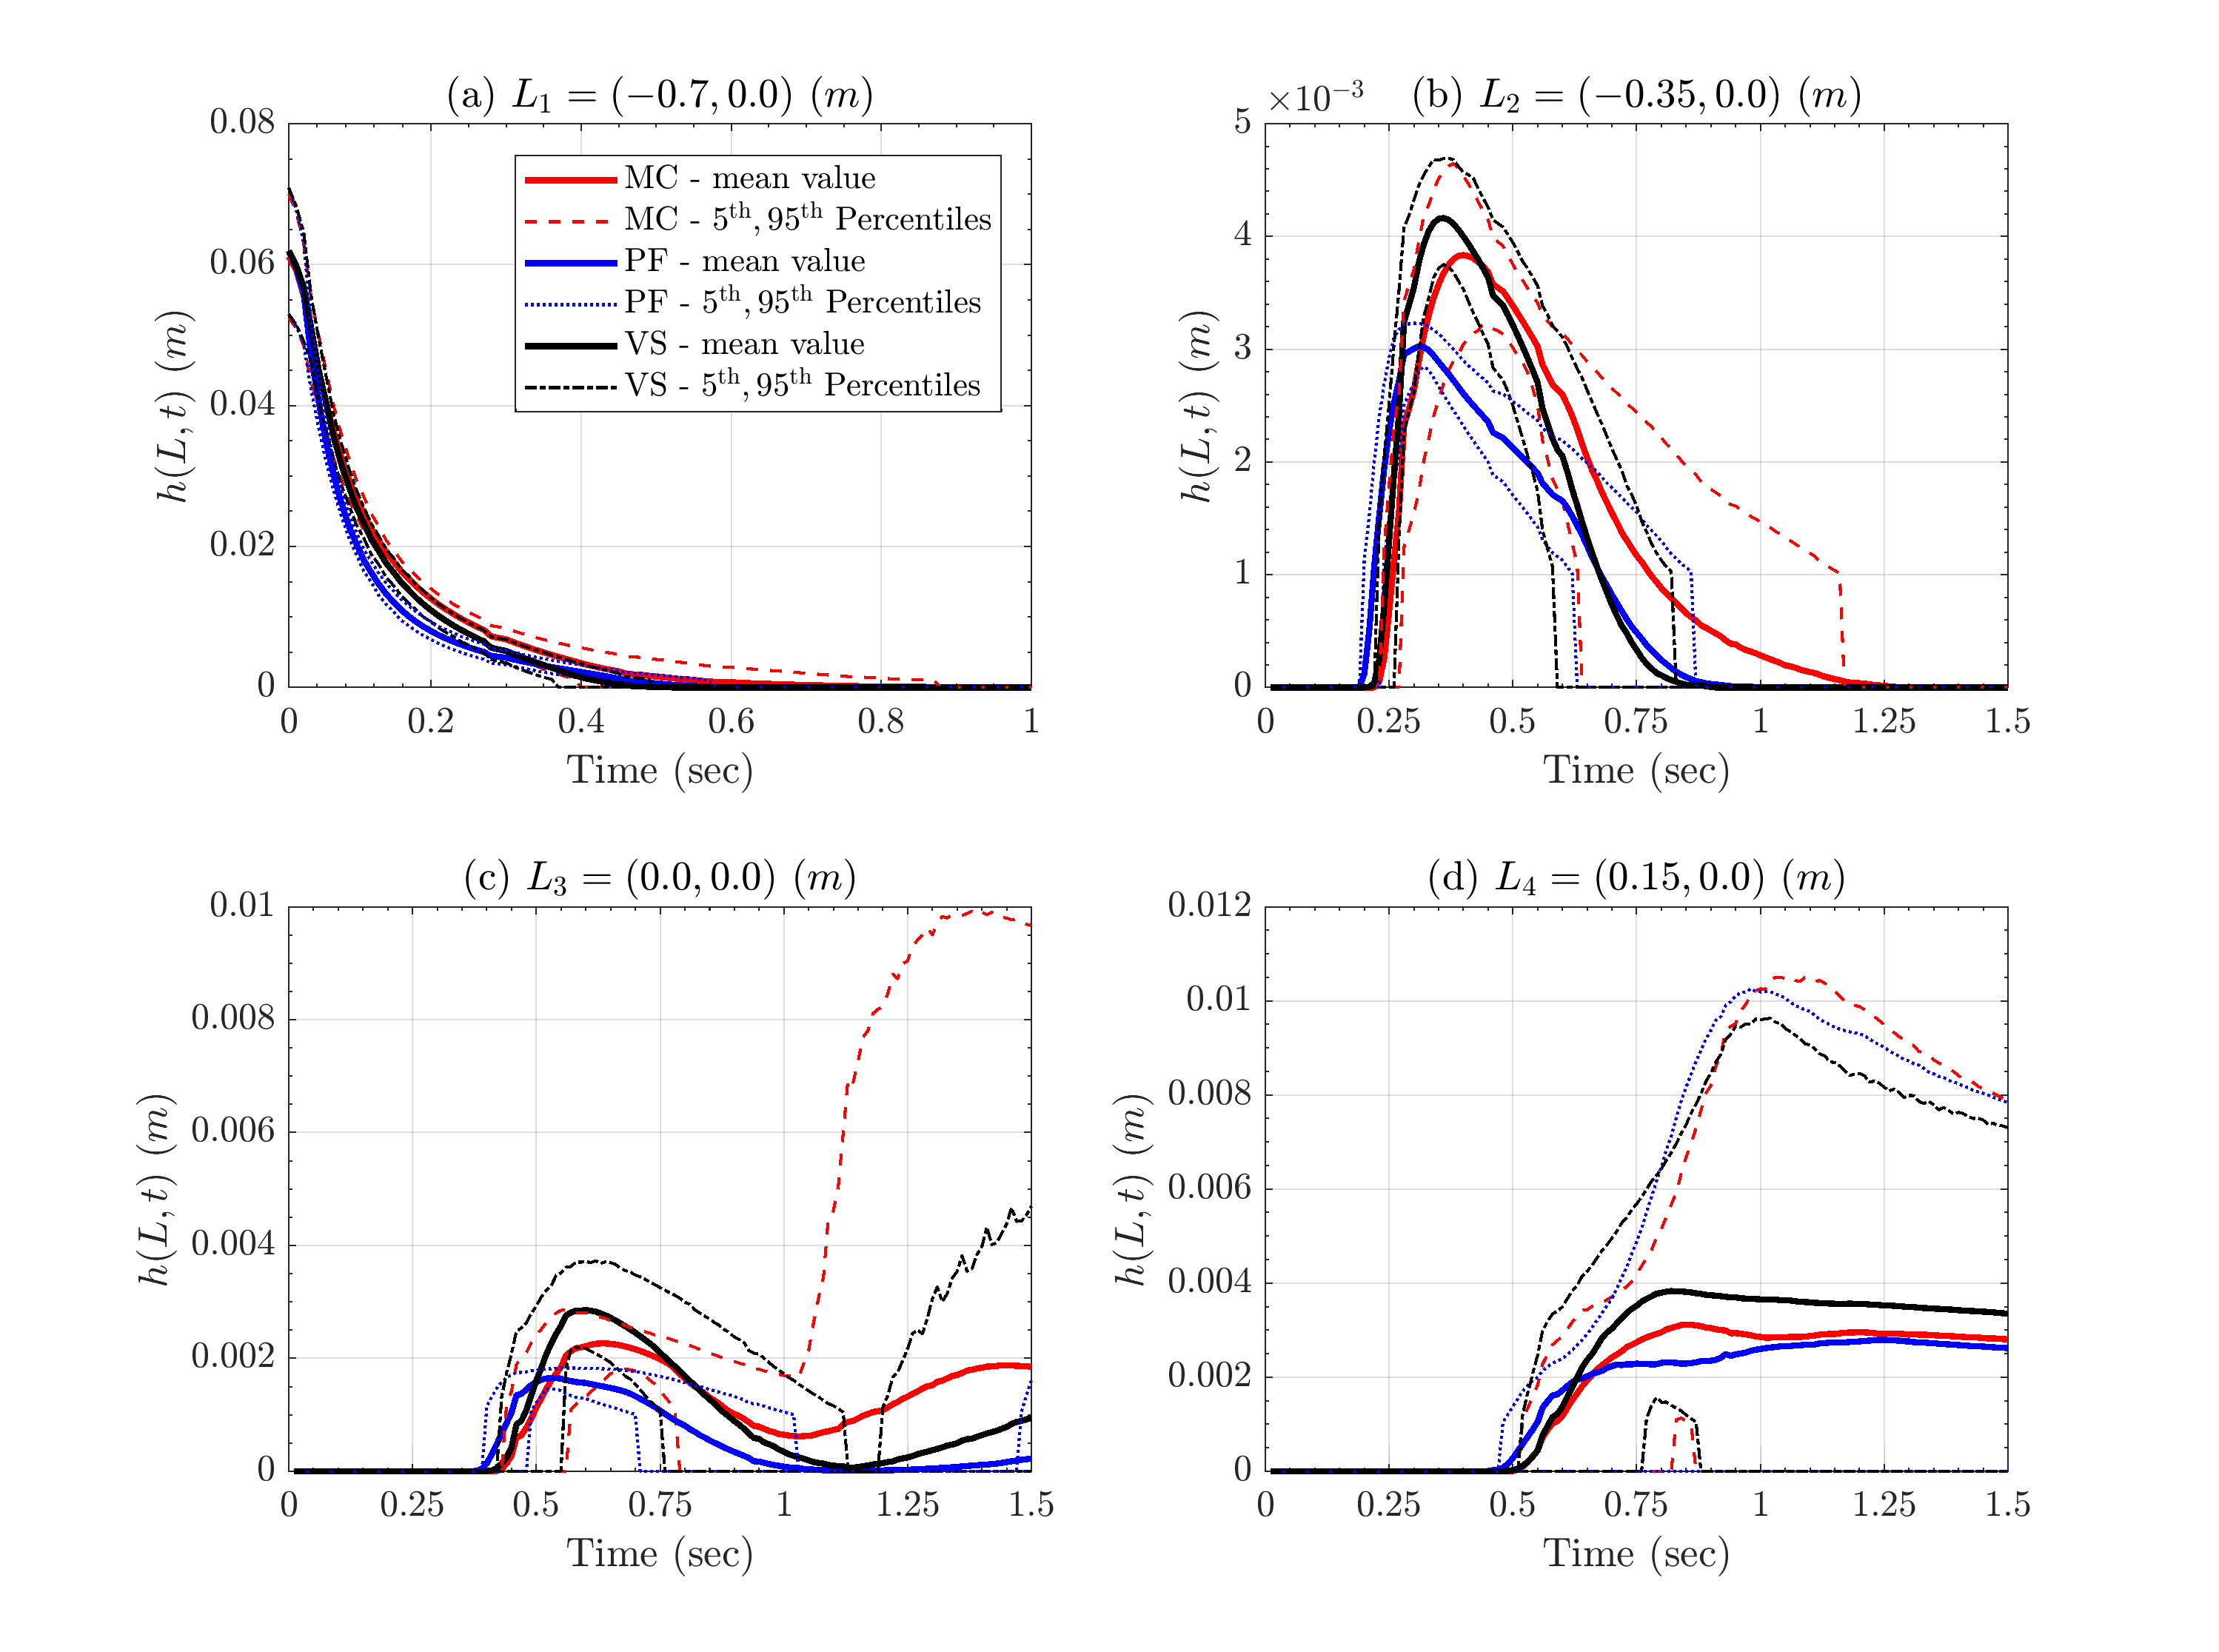
\includegraphics[width=0.9\textwidth]{InclinedPlane/LocalMeasurments/Height.png}
        \caption{Records of flow height at four spatial locations of interest. Bold line is mean value, dashed/dotted lines are 5$^{\mathrm{th}}$ and 95$^{\mathrm{th}}$ percentile bounds. Different models are displayed with different colors. Plots are at different scale, for simplifying lecture.}
        \label{fig:Ramp-H}
\end{figure}
In plot \ref{fig:Ramp-H}a, related to point $L_1$ placed on the initial pile, the values of $\sim 6\pm 1$ cm are equal and express the assigned pile height. The flow height decreases slightly faster in PF model, and slower in MC, compared to VS. Differences are more significant in plot \ref{fig:Ramp-H}b, related to point $L_2$, placed in the middle of the slope. Maximum flow height on average is greater in VS, $4.1\pm 0.2$ mm, but more uncertain in MC, $3.9\pm 0.4$ mm, and generally smaller in PF model, $3.0\pm 0.1$ mm. After the peak, PF decreases significantly slower than the other models. These height values are about 15 times smaller than initial pile height. None of the models leaves a significant material deposit in $L_1$ or $L_2$, and hence the 95$^{\mathrm{th}}$ percentile of the height is null at the ending-time. In contrast, a deposit is left at points $L_3$ and $L_4$, i.e. plot \ref{fig:Ramp-H}c placed at the change in slope, and plot \ref{fig:Ramp-H}d in the middle of the flat runway. At $L_3$ MC's deposit, $2$ mm with uncertainty [-2,+8] mm, is higher than the other models' deposits. The plot profile is bimodal, showing a first peak at $\sim 0.6$ s, and then a reduction until $1$ s, before the final accumulation. At $L_4$, deposit it is not significantly different between the three models. It measures $\sim 3$ mm on average, slightly more than this in VS, with uncertainty [-3,+7] mm.

\subsubsection{Flow acceleration}
Figure \ref{fig:Ramp-AccL} shows the flow acceleration, $\Vert \underline{\mathbf{a}} \Vert(L,t)$, at the points $(L_i)_{i=1,\dots,4}$. Acceleration is the link between force terms and observable motion. We calculated it from the left-hand-side of the dynamical equation, but using the RHS terms produces very similar results, although not identical due to the numerical approximations in solving the equations.
\begin{figure}[H]
         \centering
        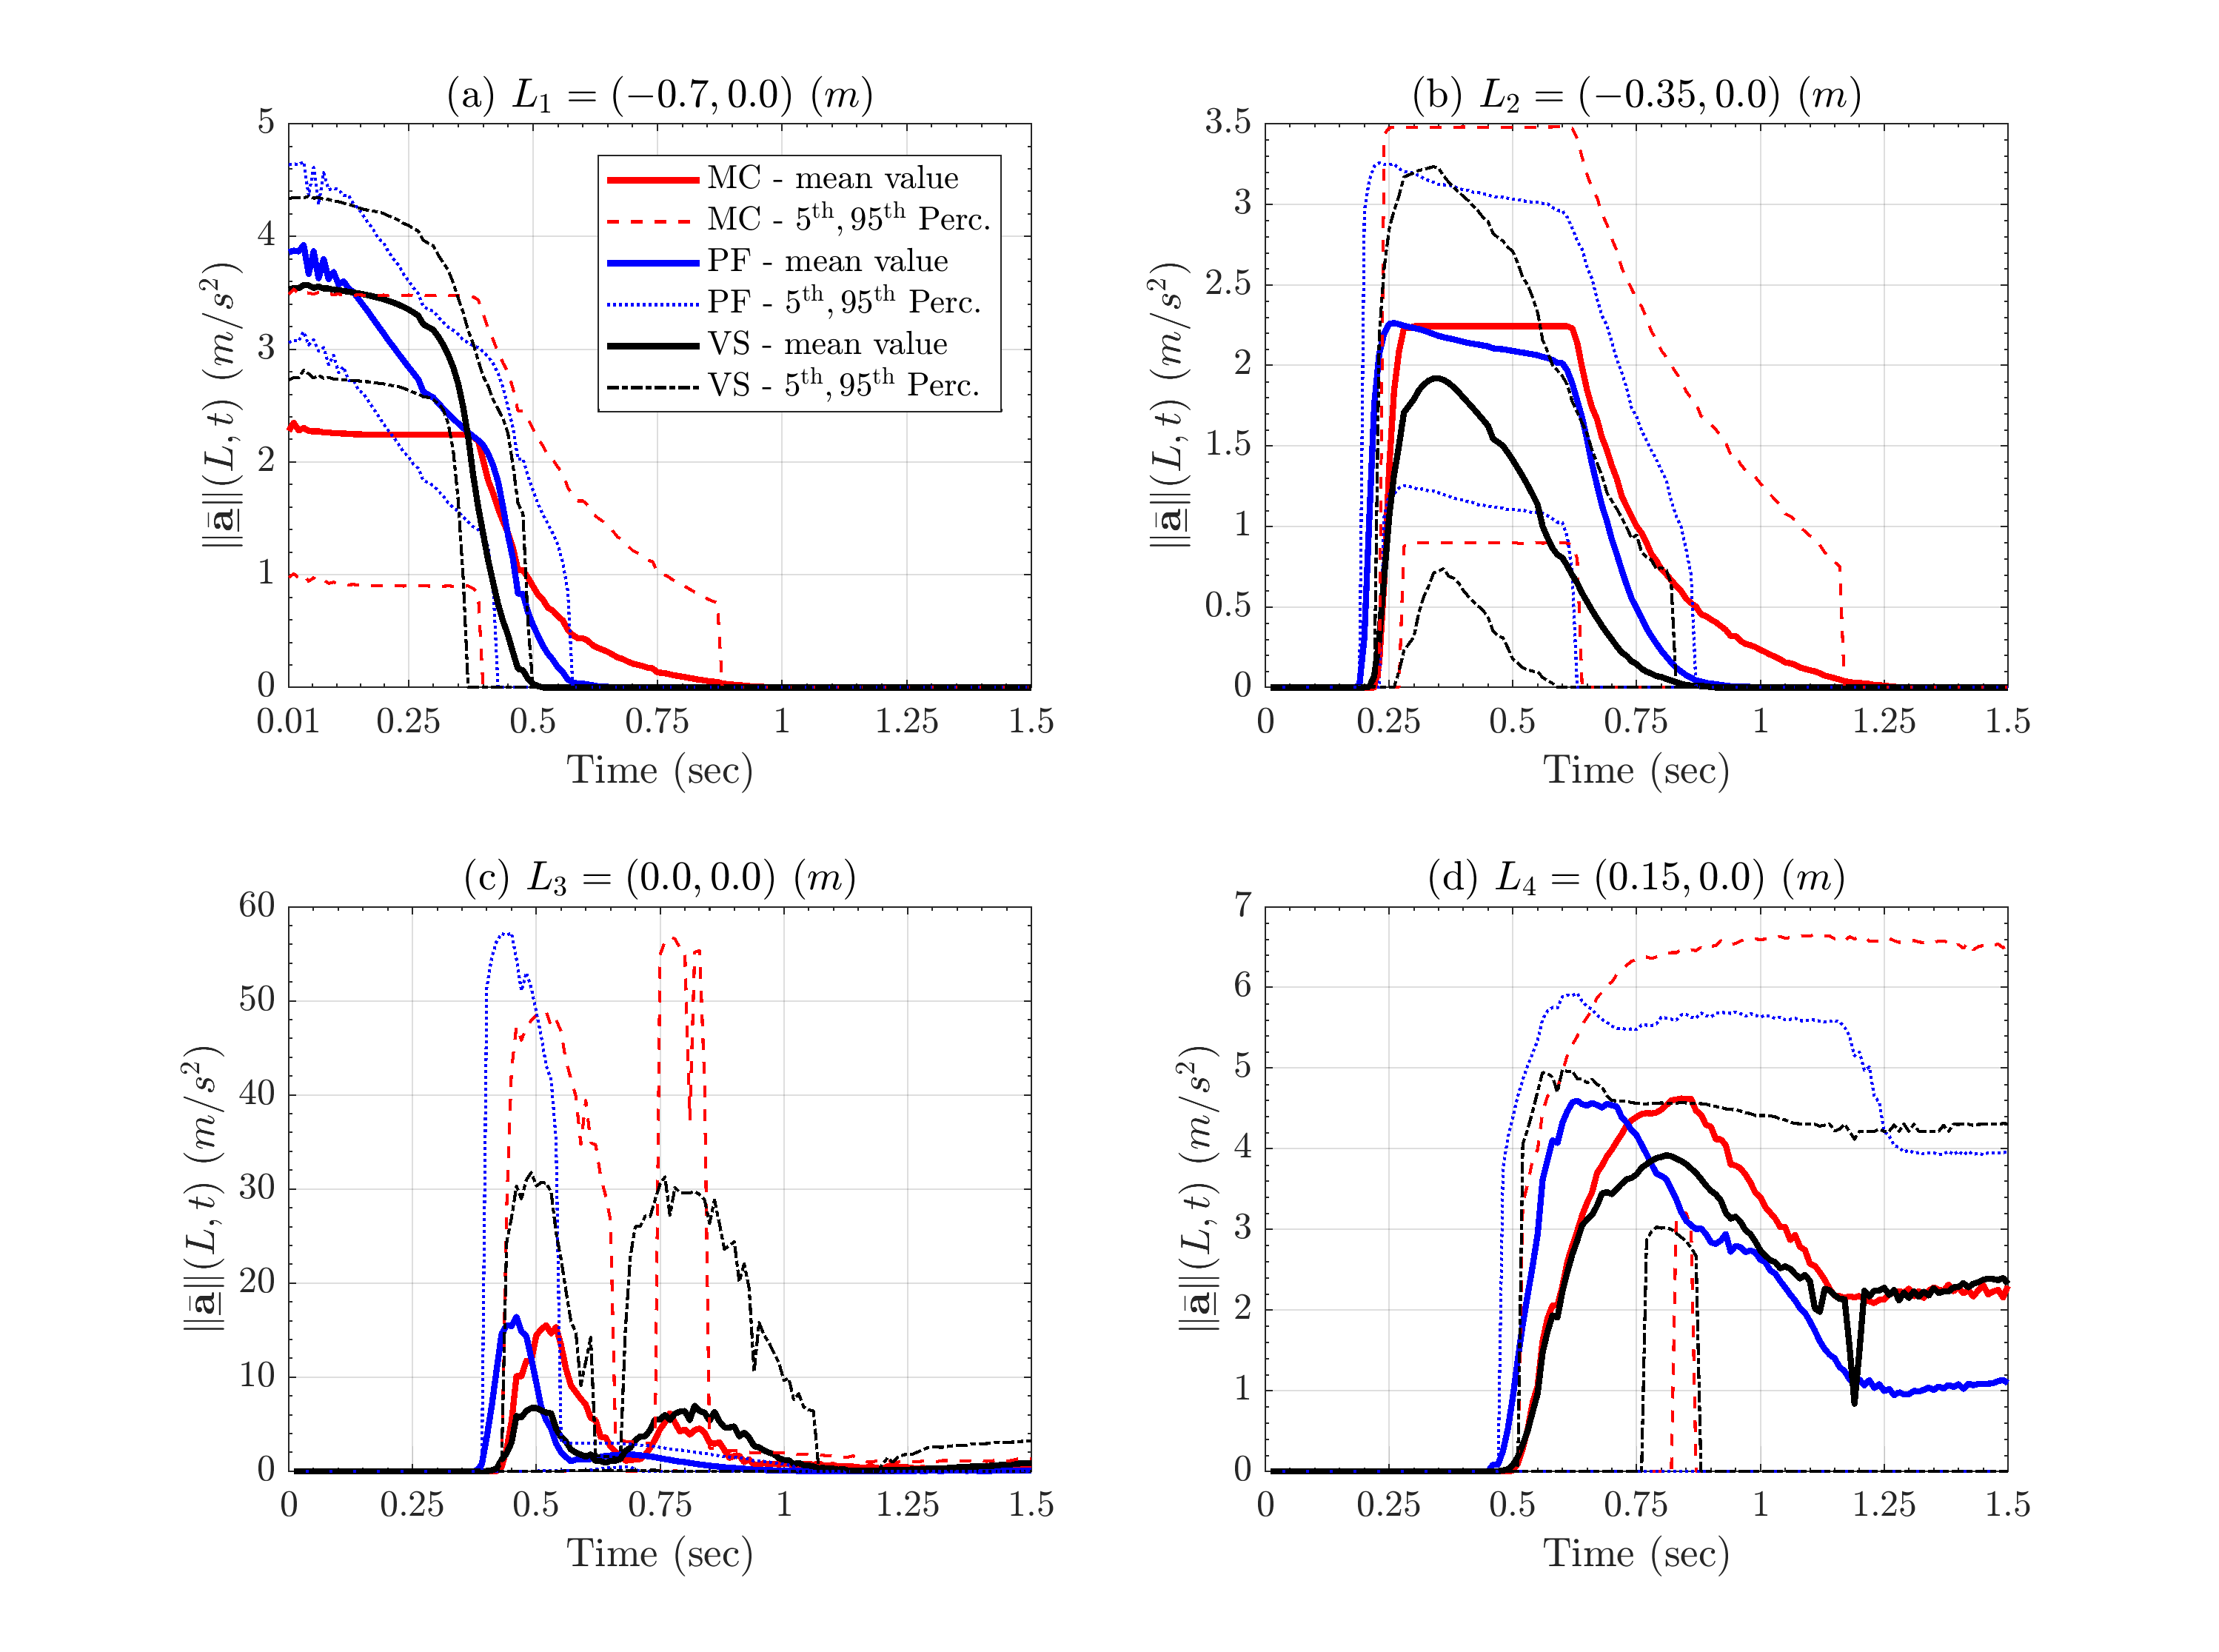
\includegraphics[width=0.9\textwidth]{InclinedPlane/LocalMeasurments/Acceleration.png}
        \caption{Records of flow acceleration modulus at four spatial locations of interest. Bold line is mean value, dashed lines are 5$^{\mathrm{th}}$ and 95$^{\mathrm{th}}$ percentile bounds. Different models are displayed with different colors. Plots are at different scale.}
        \label{fig:Ramp-AccL}
\end{figure}
In plot \ref{fig:Ramp-AccL}a, related to point $L_1$, MC and VS show a plateau before $\sim 0.4$ sec, at $\sim 2.5 \ m/s^2$ and $\sim 3.5 \ m/s^2$, respectively, while PF linearly decreases between those same values. Instead in plot \ref{fig:Ramp-AccL}b, related to point $L_2$, MC and PF show a plateau, at $\sim 2.2$ m/s$^2$, while VS has a more bell-shaped profile. UQ tells us that PF is affected by a smaller uncertainty than the other models. In plot \ref{fig:Ramp-AccL}c, related to point $L_3$, all the models show a bimodal profile, with peaks at $\sim$ 0.5 sec and 0.8 sec. This is more accentuated in MC and VS, whereas the second peak is almost absent from PF's profile. The second peak is motivated by an increase of velocity in the down-slope direction after its reduction due to lateral spreading of material. At the first peak, acceleration values are significant, with average peaks in MC and PF both at $\sim 15 \ m/s^2$, and 95$^{\mathrm{th}}$ percentile plot reaching $\sim 50 \ m/s^2$ and $\sim 55 \ m/s^2$, respectively. VS shows about halved acceleration peak values. At the second peak, average acceleration values are similar in MC and VS, at $\sim 5 \ m/s^2$. In contrast, 95$^{\mathrm{th}}$ percentile plot is $> 50 \ m/s^2$ for MC, while $\sim 30 \ m/s^2$ in VS. In plot \ref{fig:Ramp-AccL}d, related to point $L_4$, the acceleration has a first peak at $\sim 4 \ m/s^2$, and a final asymptote at $\sim 2 \ m/s^2$ in MC and VS, $\sim 1 \ m/s^2$ for PF. These values indicate flow deceleration, and uncertainty is more relevant in MC and PF than in VS.
\newpage
\subsection{Statistical analysis of latent variables}\label{Hq1}
Figure \ref{fig:Ramp-Pr_x} shows the Dominance Factors $(P_i)_{i=1,\dots,4}$, obtained projecting the RHS terms in the slope direction. The dominance factor is the probability of a force term to be the greatest one. Because these values are probabilities, they always belongs to $[0,1]$. The plots include also the probability of no-flow being observed at the considered point. The different models are plotted separately: \ref{fig:Ramp-Pr_x}a,d,g,j assume MC; \ref{fig:Ramp-Pr_x}b,e,h,k assume PF; \ref{fig:Ramp-Pr_x}c,f,i,l assume VS.
\begin{figure}[H]
         \centering
        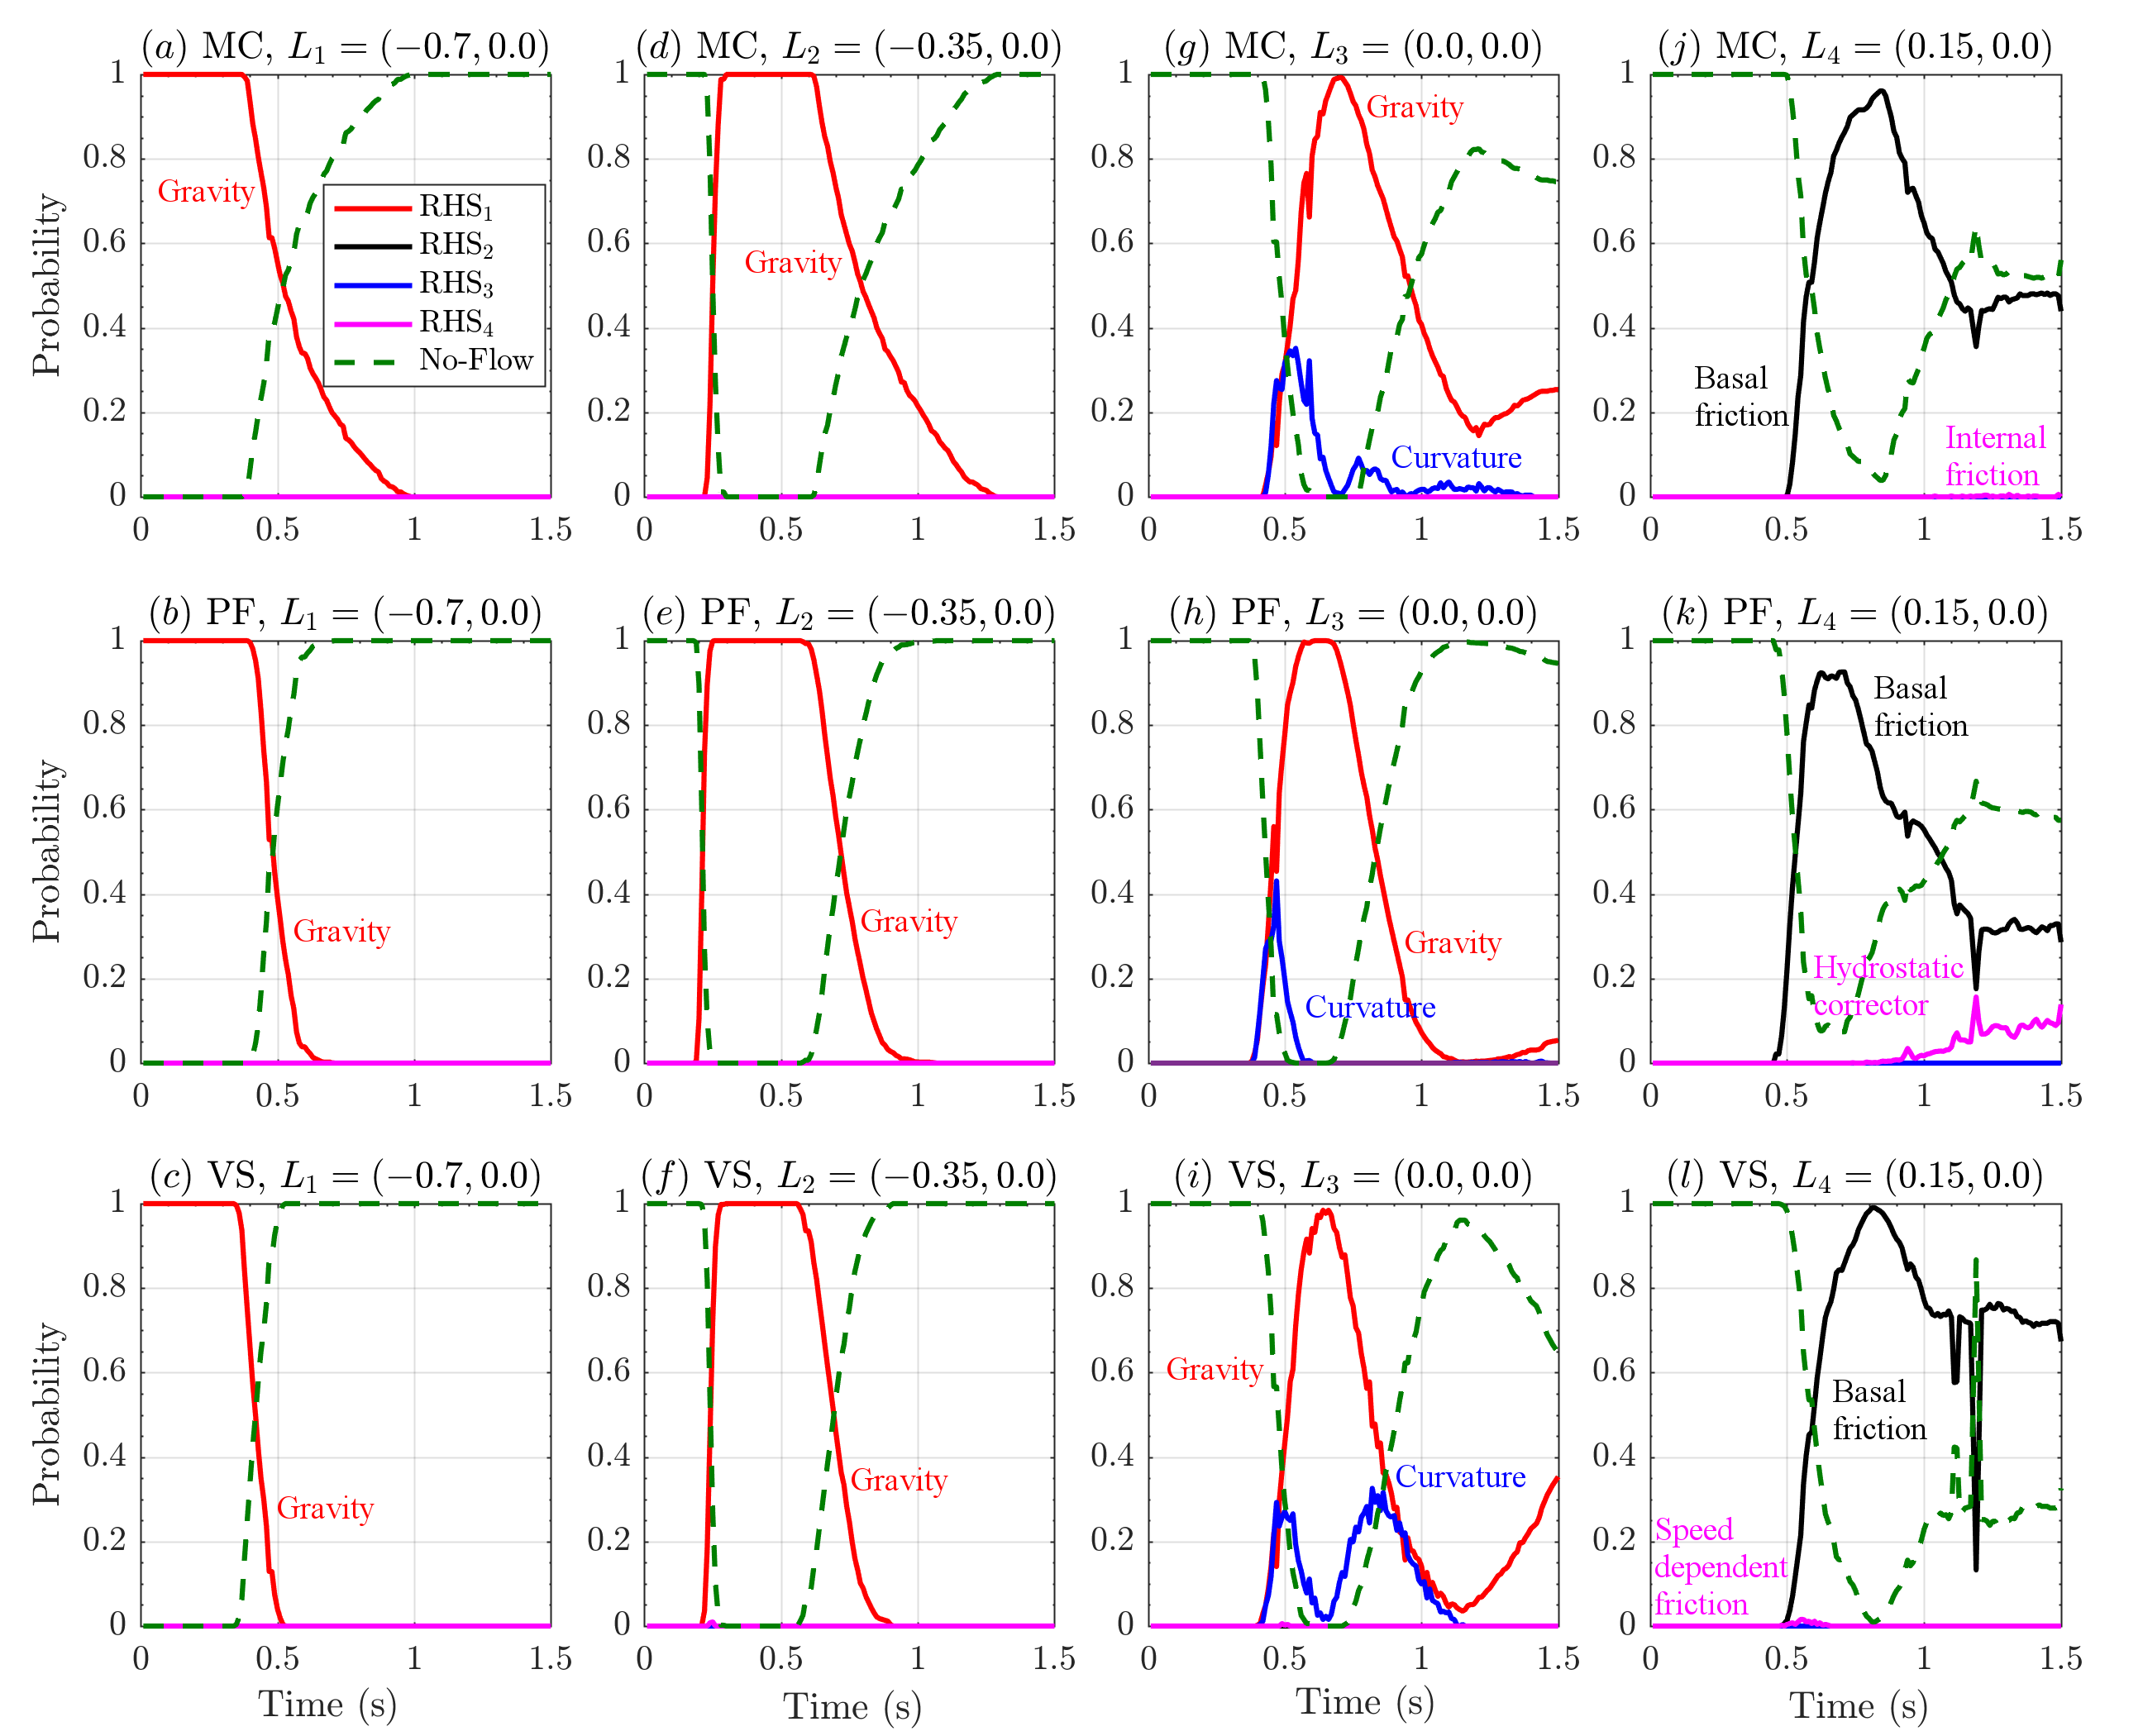
\includegraphics[width=0.95\textwidth]{InclinedPlane/ForceContrib/Pr_x.png}
        \caption{Records of dominance factors of \textbf{RHS} forces, in the slope direction, at four spatial locations of interest. Different models are displayed with different colors. No-flow probability is also displayed with a green dashed line.}
        \label{fig:Ramp-Pr_x}
\end{figure}
The plots \ref{fig:Ramp-Pr_x}a,b,c are related to point $L_1$, placed on the initial pile. Only $\boldsymbol{RHS_1}$ can be the dominant force, and no-flow probability is $(1-P_1)$. Same thing in the plots \ref{fig:Ramp-Pr_x}d,e,f related to point $L_2$, placed in the middle of the slope. Then, plots \ref{fig:Ramp-Pr_x}g,h,i are related to point $L_3$, placed at the change in slope. In $L_3$, $\boldsymbol{RHS_3}$ can be the dominant term for a short time, with a peak probability of $\sim 30\%$. Plots \ref{fig:Ramp-Pr_x}j,k,l are related to point $L_4$, placed in the middle of the flat runway. In $L_4$ only $\boldsymbol{RHS_2}$ can be the dominant term, except in PF where there is a $\sim 10\%$ chance that $\boldsymbol{RHS_4}$ is the dominant term at the ending-time.

Dominance factors provide an informative description of the main dynamics of the flow, but they cannot tell anything on the not-dominant forces. The contribution coefficients can complete the statistical description of the latent variables. They are obtained dividing the force terms by the dominant force (see Appendix B). This is a tool to compare the different force terms, scaling the plots by the dominant dynamics - they belong to $[-1,1]$. It also represent the degree of relevance of the assumptions behind the force terms, changing as a function of time. Figure \ref{fig:Ramp-Ci_x} shows the Contribution Coefficients $(C_i)_{i=1,\dots,4}$, for the three rheology models. The different models are plotted separately: \ref{fig:Ramp-Ci_x}a,d,g,j assume MC; \ref{fig:Ramp-Ci_x}b,e,h,k assume PF; \ref{fig:Ramp-Ci_x}c,f,i,l assume VS.
\begin{figure}[H]
         \centering
        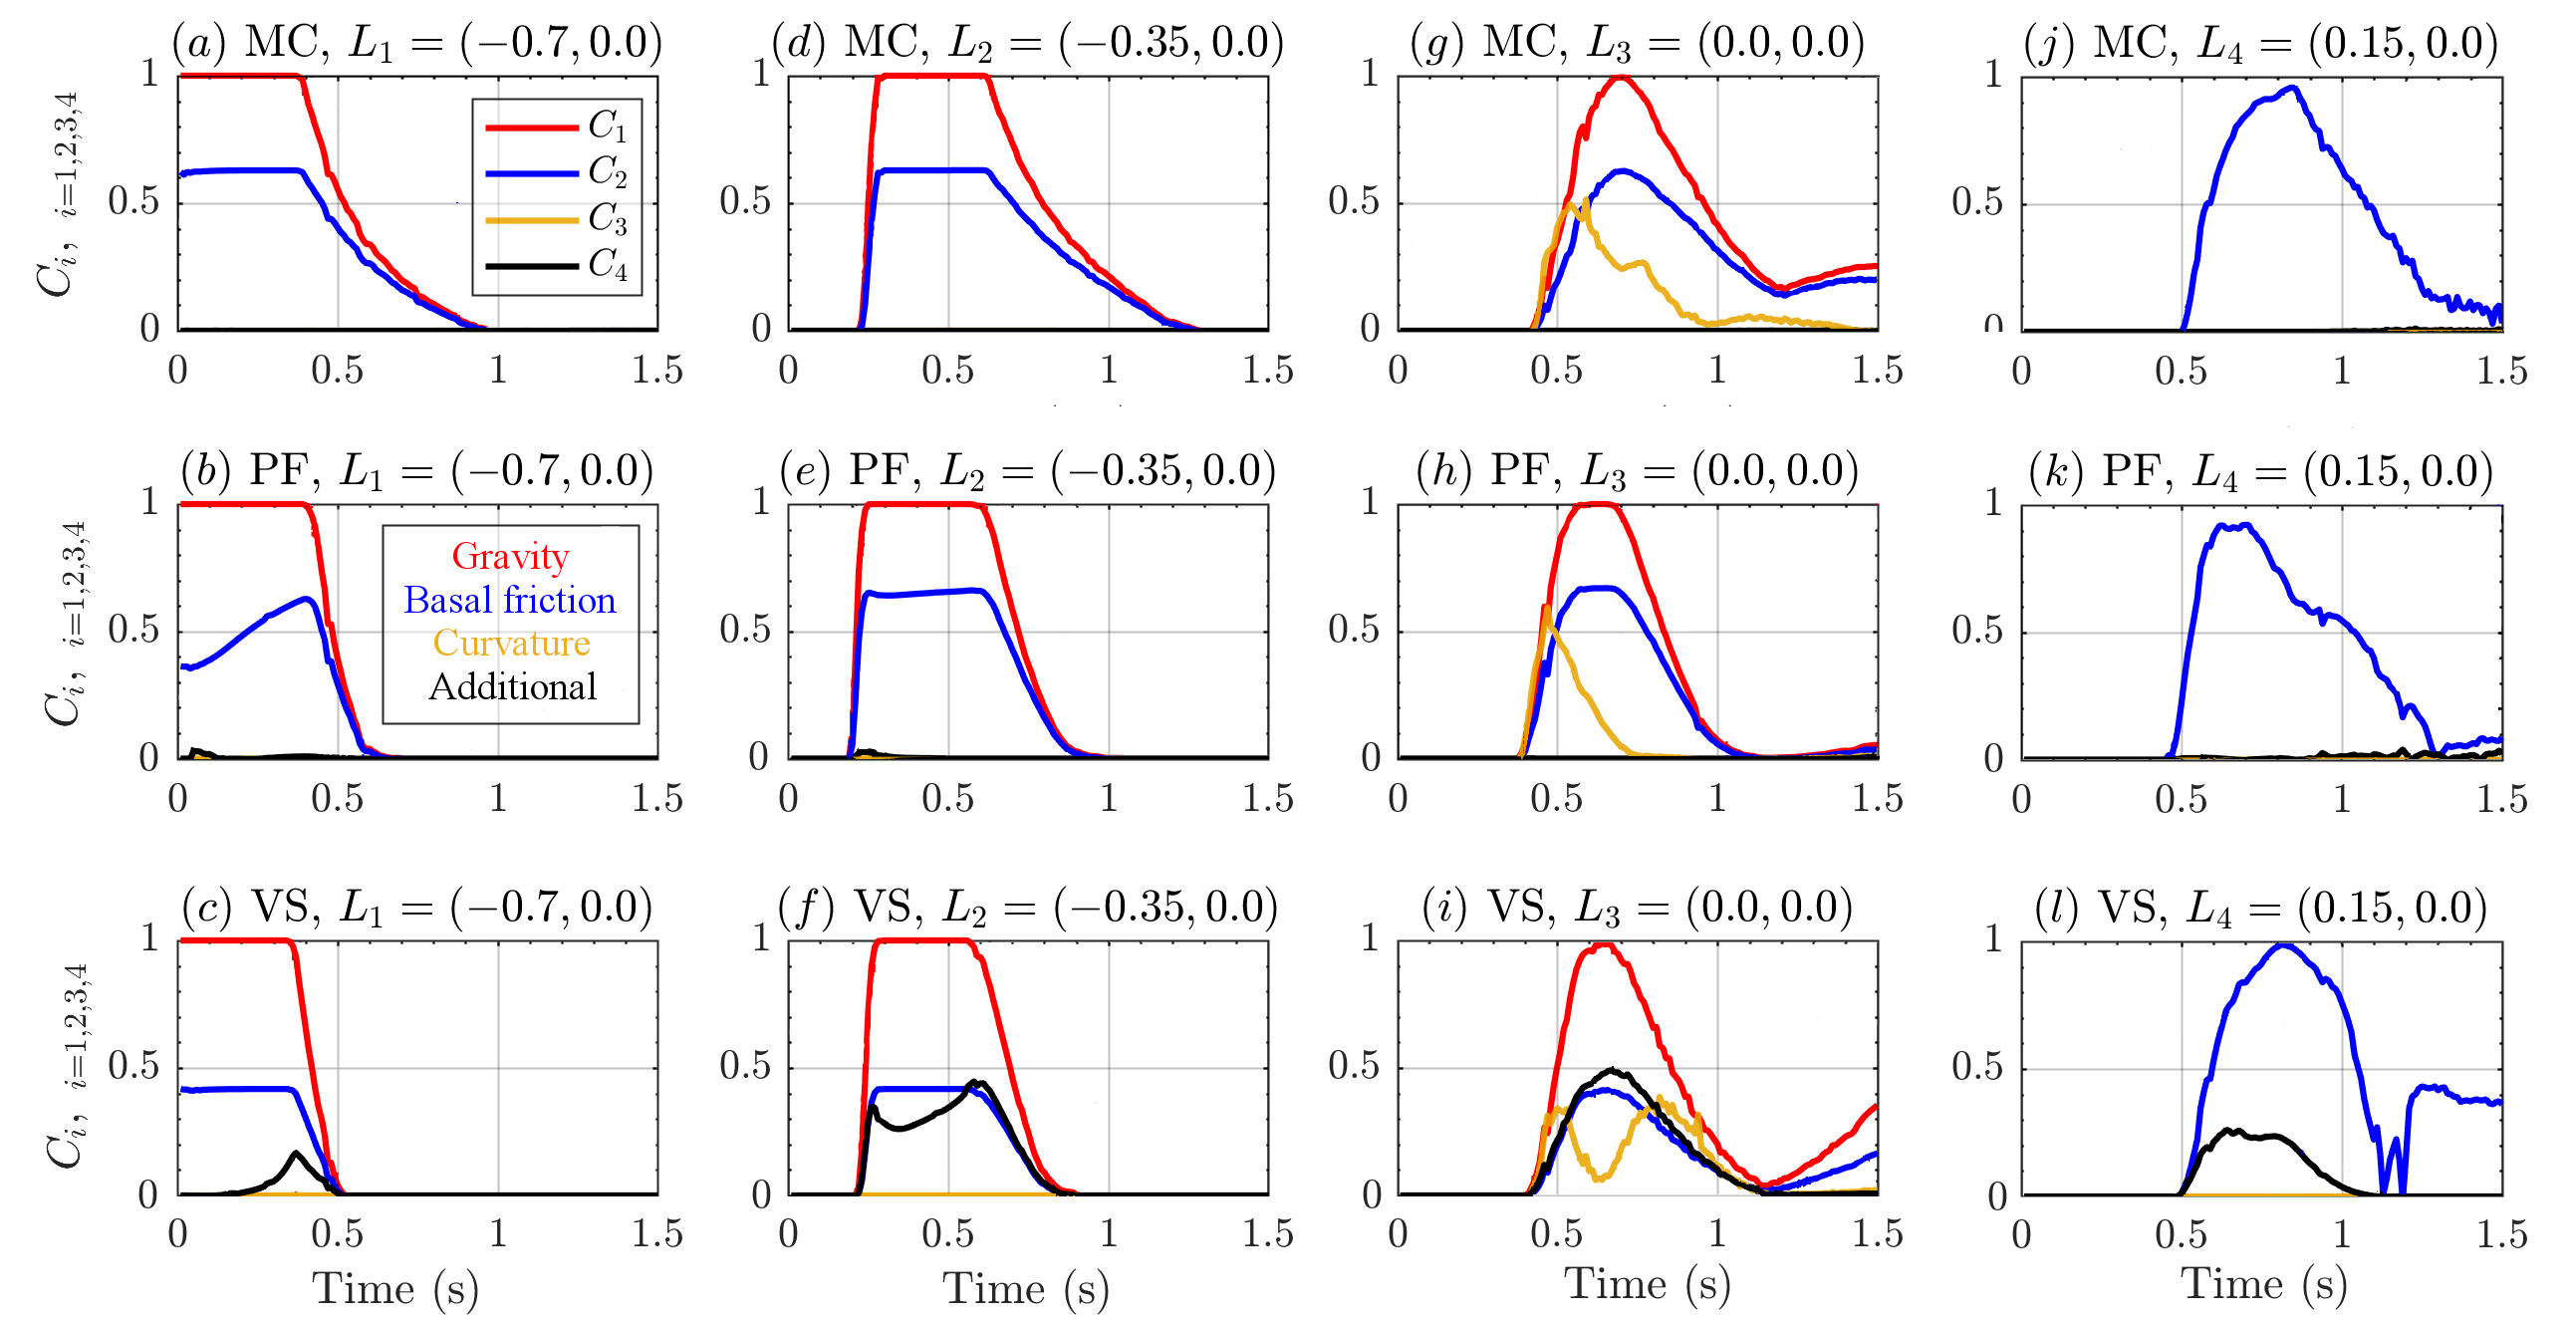
\includegraphics[width=1\textwidth]{InclinedPlane/ForceContrib/Ci_x.png}
        \caption{Records of contribution coefficients of \textbf{RHS} forces, in the slope direction, at four spatial locations of interest. Different models are displayed with different colors.}
        \label{fig:Ramp-Ci_x}
\end{figure}
The plots \ref{fig:Ramp-Ci_x}a,b,c are related to point $L_1$, placed on the initial pile. $C_1$ and $C_2$ give the major contributions, with a minor contribution from $C_4$ in VS. In general, contributions profiles are flat plateaus that start to wane after $0.4 s$, with the rise of the probability of no-flow at the point $L_1$. The plots \ref{fig:Ramp-Ci_x}d,e,f are related to point $L_2$, placed in the middle of the slope. Again the major contributions are $C_1$ and $C_2$, with trapezoidal profile preceded and followed by no-flow. In VS, $C_4$ becomes as a significant as $C_2$, but it is bimodal instead than trapezoidal. The plots \ref{fig:Ramp-Ci_x}g,h,i are related to point $L_3$, placed at the change in slope. The contributions $C_1$ and $C_2$ are still the largest, but their profiles are bell-shaped. In VS, $C_4$ is almost identical to $C_2$. In all the models, $C_3$ is also significant, with a peak similar to $C_2$, but has a different profile - triangular for MC and PF, bimodal for VS. In MC the decrease occurs in two stages. Due to the presence of deposit, all the contributions are small (particularly small in PF), but not zero at the ending time. The plots \ref{fig:Ramp-Ci_x}j,k,l are related to point $L_4$, placed in the middle of the flat runway. Only $C_2$ has a major role, with a bell shaped profile faster to wax than to wane. Contribution $C_4$ has a minor role in VS and PF.
\newpage
\subsection{Flow extent and spatial integrals}
Figure \ref{fig:Ramp-spatial} shows the spatial average of speed and Froude Number. Moreover, it shows the lateral extent and inundated area of flow, as a function of time. These global quantities have smoother plots than the local measurements describe above. However, most of the details observed in local measurements are not easy to discern.
\begin{figure}[H]
        \centering
        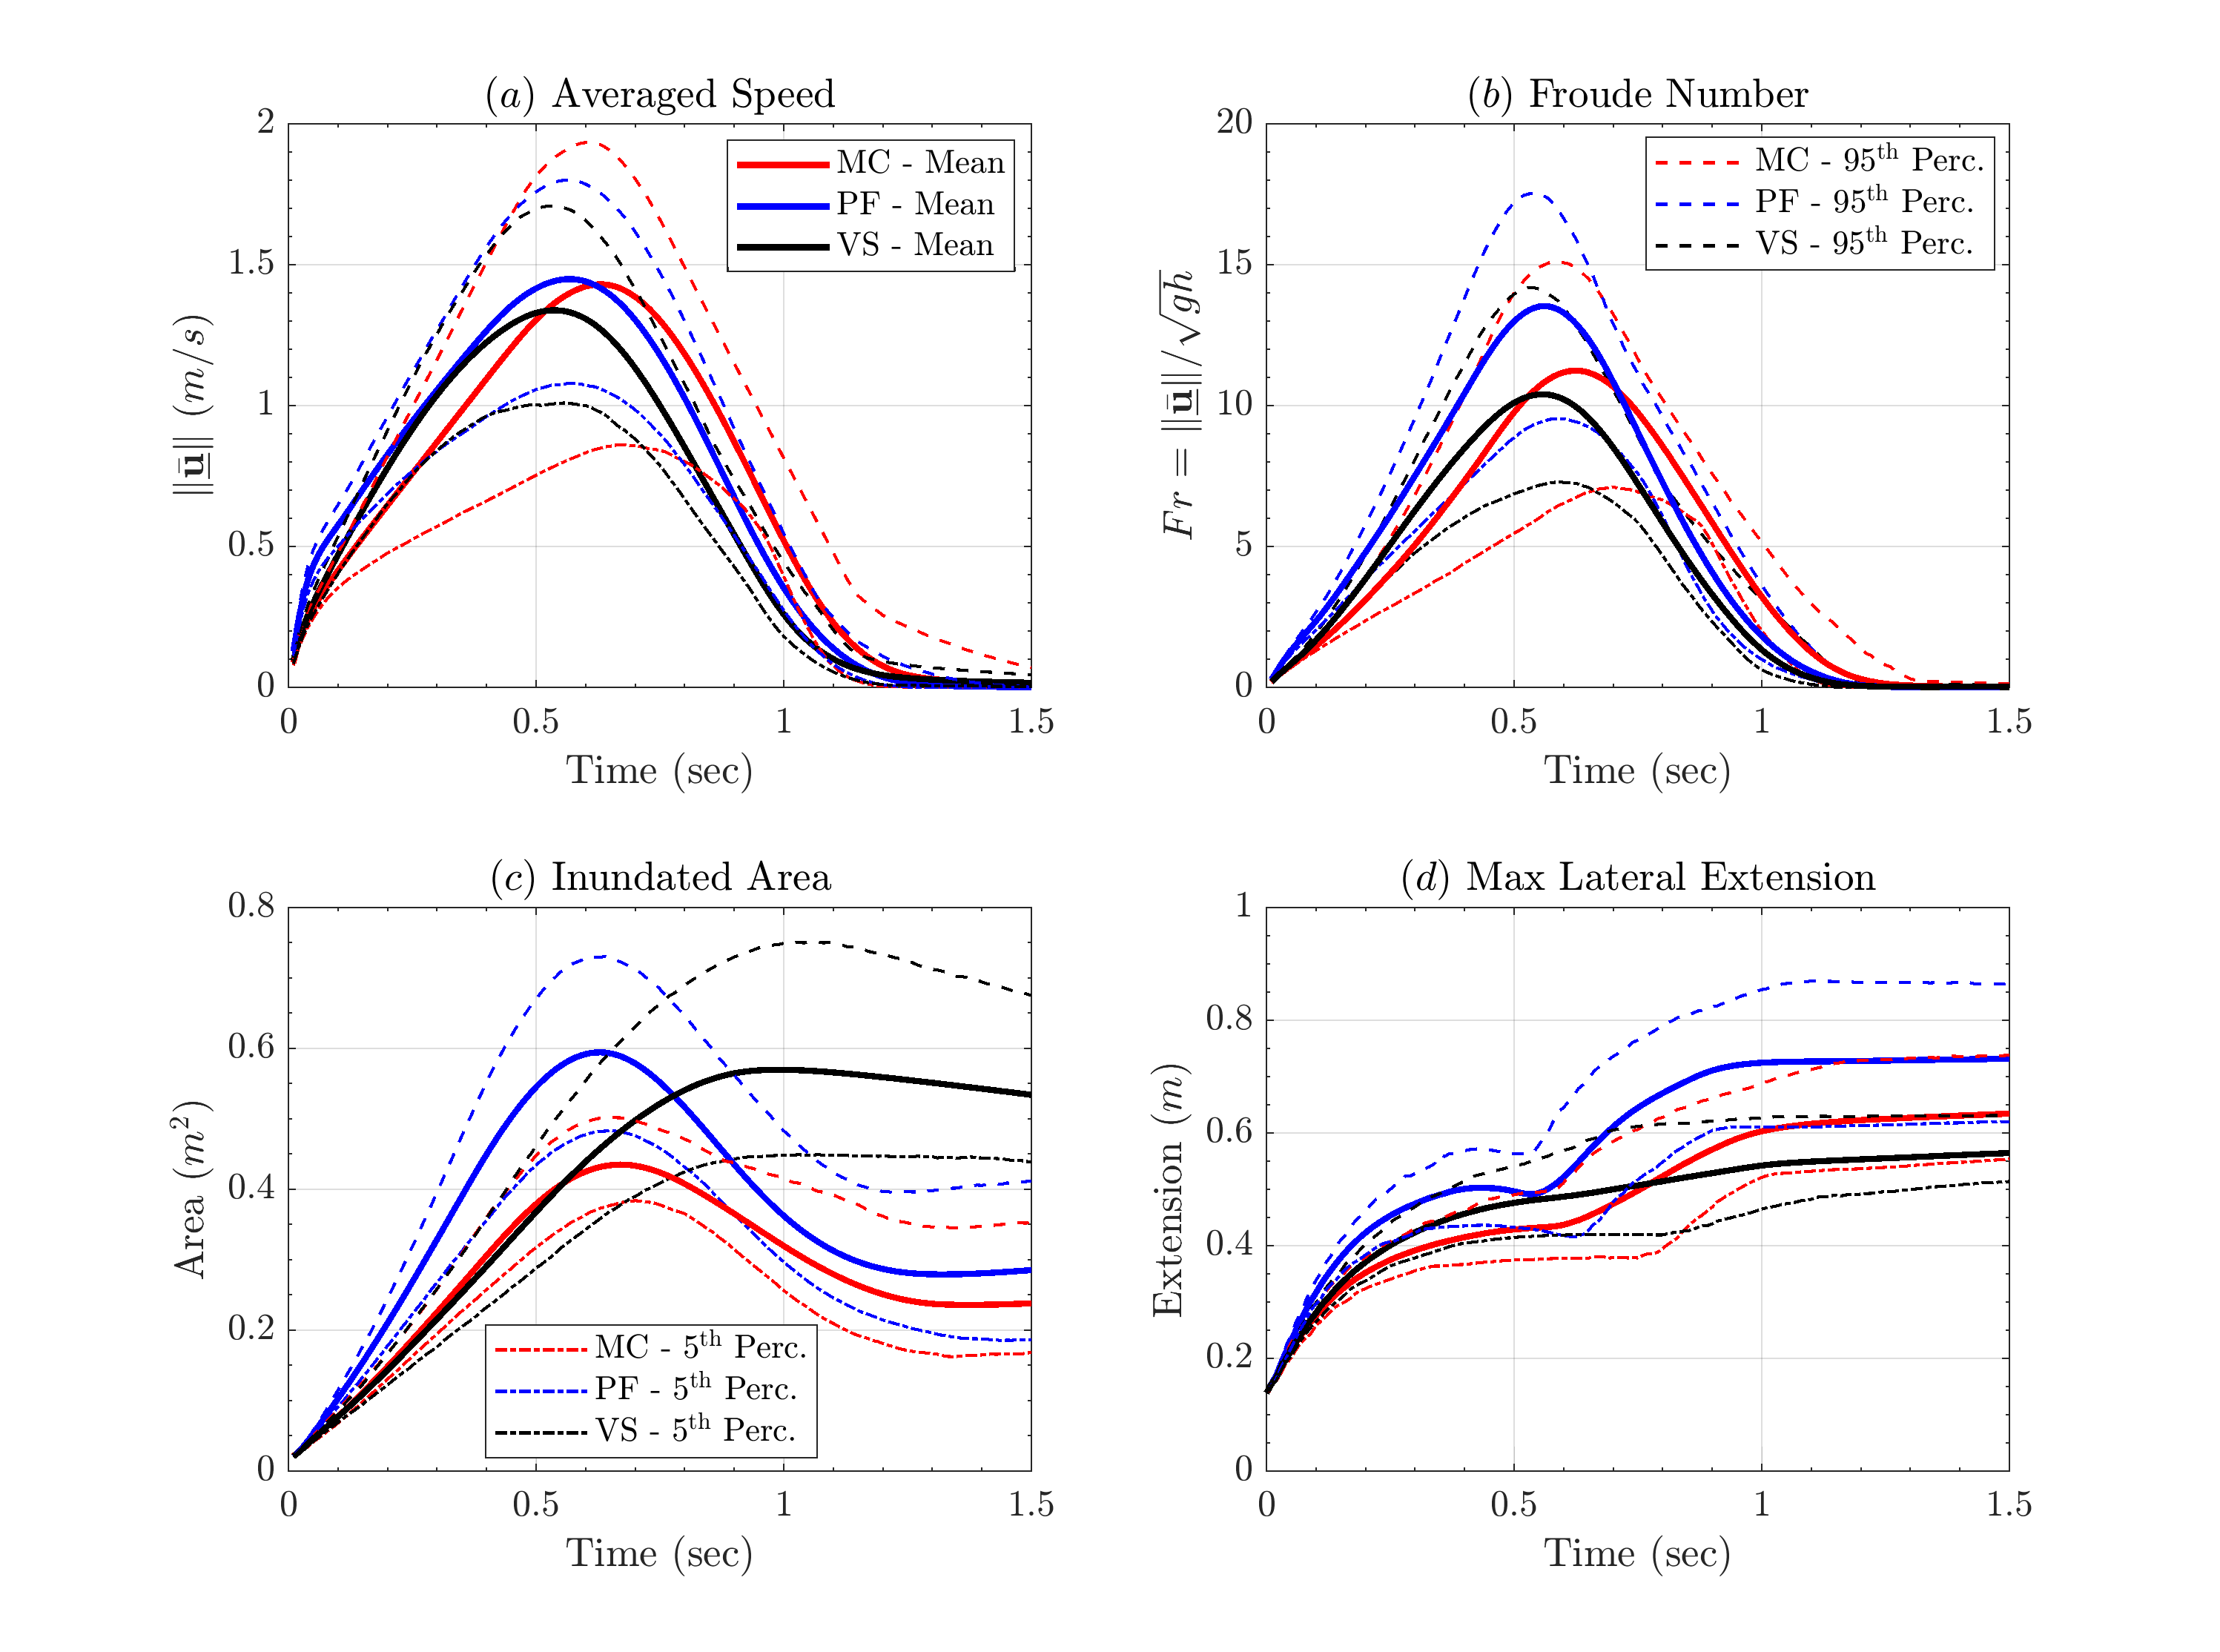
\includegraphics[width=0.85\textwidth]{InclinedPlane/AveragedMeasurments/Averaged_MeasuresIncline.png}
        \caption{Comparison between spatial averages of $(a)$ flow speed, and $(b)$ Froude Number in addition to the flow $(c)$ lateral extent, and $(d)$ inundated area, as a function of time. Different models are displayed with different colors.}
        \label{fig:Ramp-spatial}
\end{figure}
In plot \ref{fig:Ramp-spatial}a the speed has a bell-shaped profile in all the models, with an average peak at $\sim 1.4 m/s$ and uncertainty range of $\pm 0.4 m/s$ for PF and VS. VS is slightly slower, reaching $\sim 1.3 m/s$ on average. MC shows a larger uncertainty range, of $\pm 0.6 m/s$. The maximum speed is reached first by VS and PF at $\sim 0.55 s$, and last by MC at $\sim 0.65 s$. In plot \ref{fig:Ramp-spatial}b, also the Froude Number has a bell-shaped profile. $Fr$ peaks are temporally aligned with speed peaks, and are $\sim 10$ in VS, $\sim 11$ in MC, $\sim 13.5$ in PF, on average. Uncertainty range is about $\pm 4$ in all models. In plot \ref{fig:Ramp-spatial}c inundated area shows similar maximum values in PF and VS, at $\sim 0.6 m^2$ on average, and uncertainty of $\pm 0.15 m^2$. MC is lower, at $\sim 0.45 m^2$ on average, and less uncertain, $\pm 0.10 m^2$. VS does not decrease significantly after reaching the peak, whereas the other models contract their area to approximately half its maximum extent. In plot \ref{fig:Ramp-spatial}d the lateral extent starts equal to the pile diameter $\sim 15 cm$, and then rises in two stages in MC and PF. The second and greater rise starts at $\sim 0.6 s$, and corresponds with the time of arrival at the change in slope (see Fig. \ref{fig:Ramp-H}c). In contrast, VS rises without showing two phases. At $\sim 0.6 s$, average lateral extent is $\sim 50 cm$ in PF and VS, and $\sim 43 cm$ in MC. Uncertainty range is $\pm 7 cm$ for all models at that time. Final extent is $\sim 75 cm$ in PF, $\sim 65 cm$ in MC, $\sim 55 cm$ in VS. Uncertainty range is $\pm 5 cm$ in VS, but rises to $\pm 10 cm$ in MC and PF.

\subsubsection{Power integrals}
Figure \ref{fig:Ramp-Power-spatial} shows the spatial integral of powers. The spatial integration is performed on half spatial domain, due to the symmetry with respect to the flow central axis. In particular, the power estimates assume a material density $\rho = 805 kg/m^3$. This a fixed scaling factor, and the plots aspect is not affected by its value. Corresponding plots of the force terms are included in Supporting Information S2.
\begin{figure}[H]
        \centering
        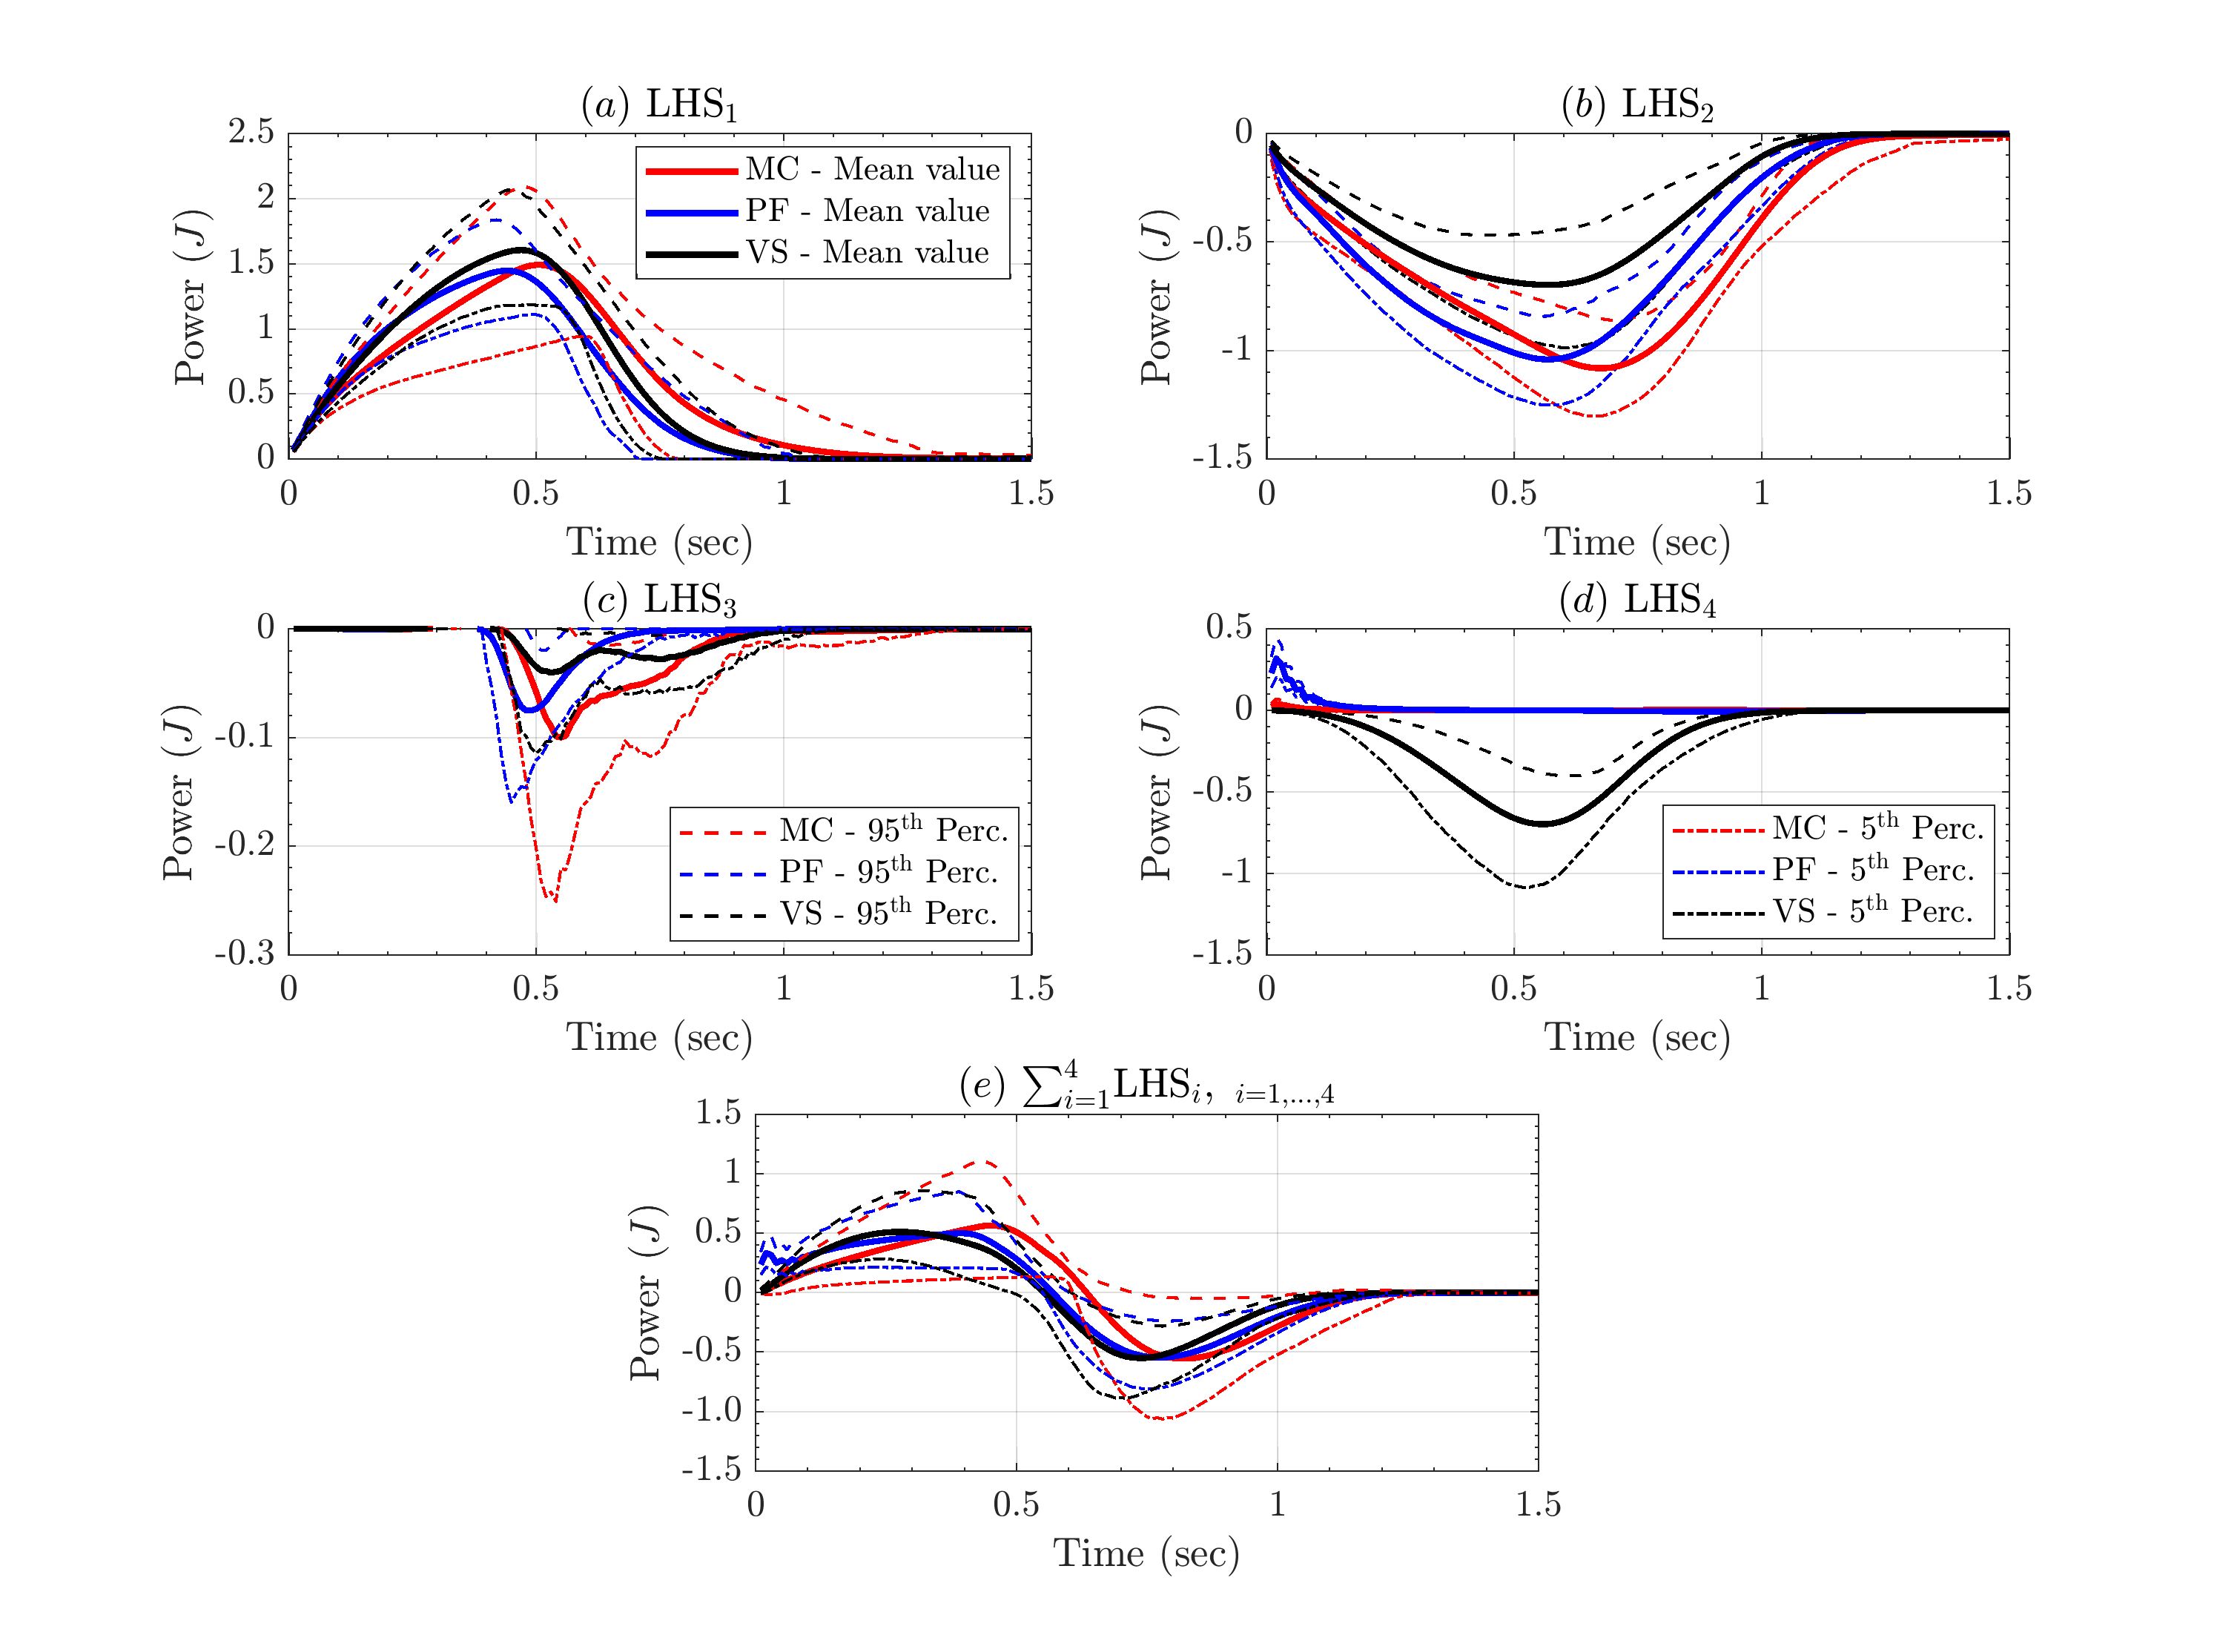
\includegraphics[width=0.95\textwidth]{InclinedPlane/AveragedMeasurments/PowersIncline.png}
        \caption{Spatial integral of the RHS powers. Bold line is mean value, dashed lines are 5$^{\mathrm{th}}$ and 95$^{\mathrm{th}}$ percentile bounds. Different models are displayed with different colors.}
        \label{fig:Ramp-Power-spatial}
\end{figure}
The scalar product with velocity imposes a bell-shaped profile, as observed in Fig. \ref{fig:Ramp-spatial}a. In plot \ref{fig:Ramp-Power-spatial}a the power of $\boldsymbol{RHS_1}$ represents the effect of the gravity in all the models. It starts from zero and rises up to $\sim 1.5 W$ at $\sim 0.55 s$, then decreases to zero after the material crosses the change in slope. Uncertainty range of $\pm 0.5 W$ affects the peak values. MC decreases slower than the other models, and has a more significant uncertainty after the change in slope. PF decreases faster. In plot \ref{fig:Ramp-Power-spatial}b the power of  $\boldsymbol{RHS_2}$ represents the basal friction. It is negative and peaks to $\sim 1.1 \pm 0.2 W$ in MC, $\sim 1.0 \pm 0.2 W$ PF, $\sim 0.7 \pm 0.3 W$ in VS. A similar bell-shaped profile is shared by the three models, and basal friction power becomes negligible at the ending-time. In plot \ref{fig:Ramp-Power-spatial}c the power of $\boldsymbol{RHS_3}$ is related to the curvature effects, and it is not null only at the change in slope. It is always dissipative, i.e. opposed to flow velocity, because it is equivalent to the friction due to the additional weigh generated by centrifugal forces. It is weaker than $-0.1 W$ on average, ten times smaller than the previous powers, although MC lower percentile reaches $\sim -0.25 W$. VS displays a bimodal profile, with a second and weaker peak at $\sim 0.75 s$. In plot \ref{fig:Ramp-Power-spatial}d the power of $\boldsymbol{RHS_4}$ is related to the additional forces of the models, differently characterized. This term is really relevant in VS, although also in PF has a very short lasting positive peak up to $0.3 W$ before to become null at $\sim 0.1 s$. This power in VS is a speed dependent term, always dissipative. It is bell shaped and null before $\sim 0.1 s$ and after $\sim 1 s$. At the time of change in slope it is $\sim -0.7 W$, $\pm 0.3 W$.
\newpage
\section{Large scale flow on the SW slope of Volc{\'a}n de Colima}\label{QoI2}
Our second case study is a geophysical flow down the SW slope of Volc{\'a}n de Colima (MX) - an andesitic stratovolcano that rises to 3,860 m above sea level, situated in the western portion of the Trans-Mexican Volcanic Belt (Fig. \ref{fig:Colima-first}).
\begin{figure}[H]
    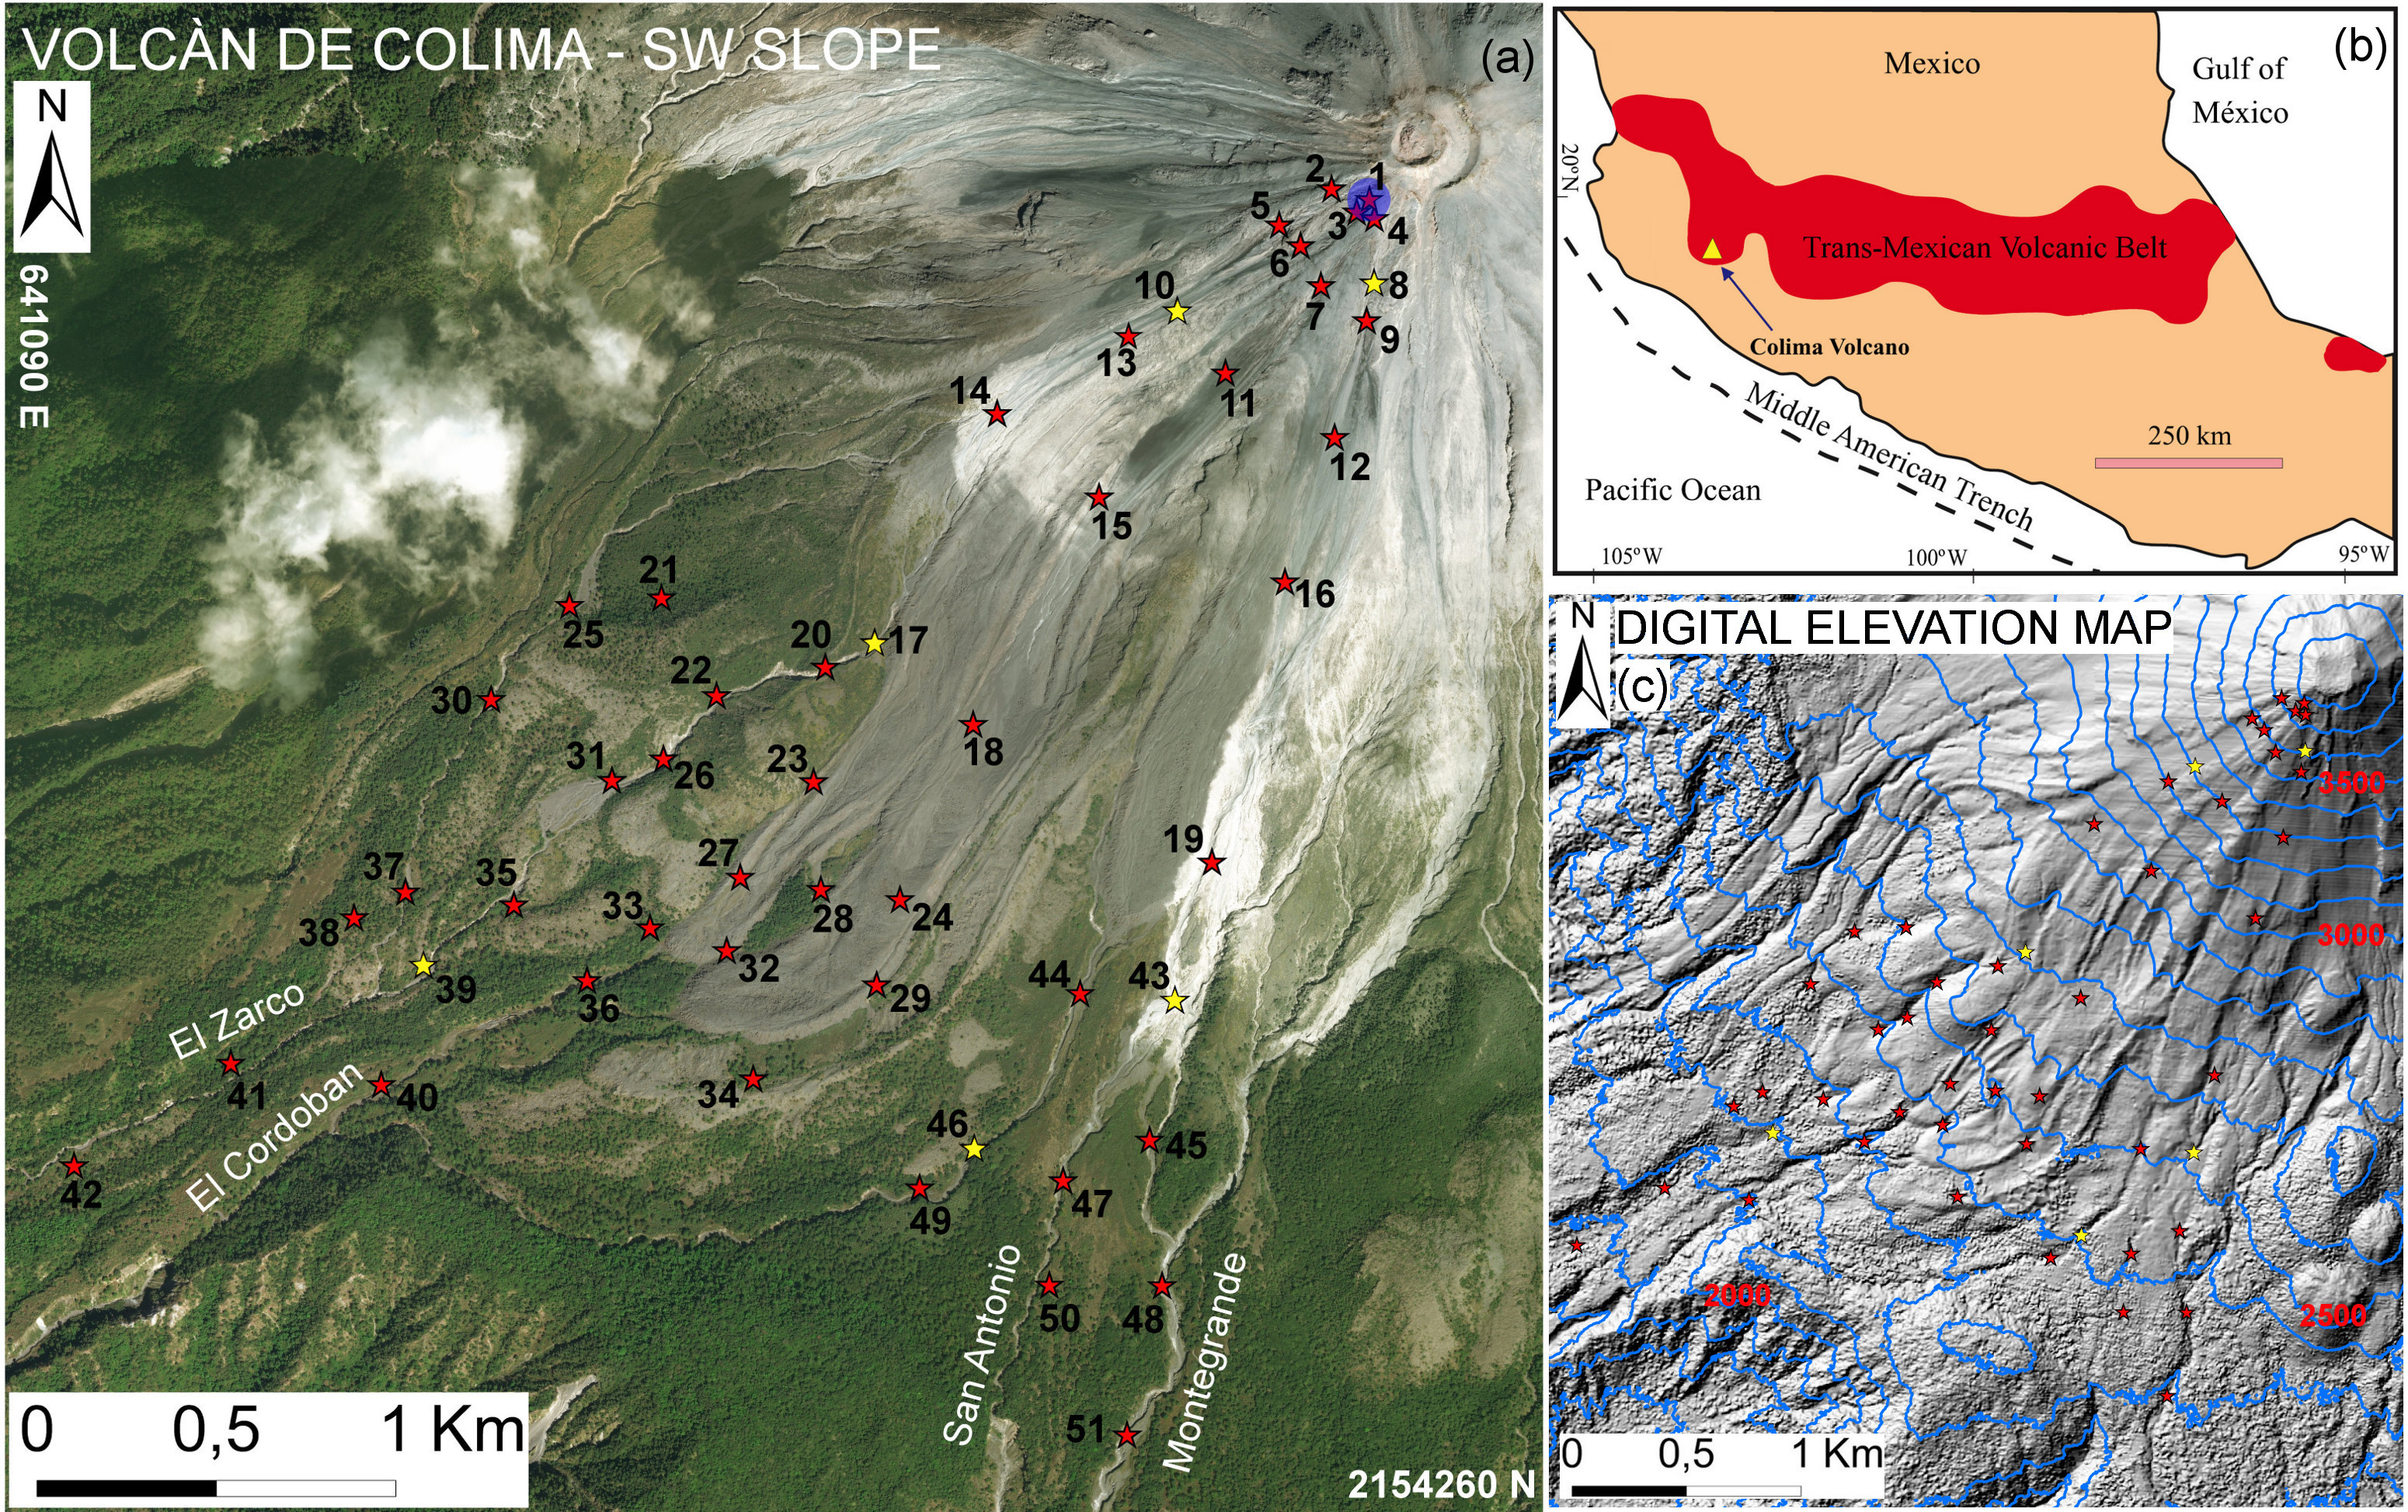
\includegraphics[width=0.9\textwidth]{BAF_VolcanDeColima/ColimaFig.jpg}
    \centering
    \caption{(a) Volc{\'a}n de Colima (M{\'e}xico) overview, including 51 numbered local sample sites (stars) and major ravines. Pile location is marked by a blue dot. Reported coordinates are in UTM zone 13N. Background is a satellite photo. (b) Regional geology map. (c) Digital elevation map. Six preferred locations are colored in yellow. Elevation isolines are included in blue, elevation values in red.}
    \label{fig:Colima-first}
\end{figure}
Volc{\'a}n de Colima has historically been the most active volcano in M{\'e}xico \citep{DeLaCruzReina1993, Zobin2002, Gonzalez2002}. The modeling of pyroclastic flows generated by explosive eruptions and lava dome collapses of Volc{\'a}n de Colima is a well studied problem \citep{DelPozzo1995,Sheridan1995,Saucedo2002,Saucedo2004,Saucedo2005,Sarocchi2011,Capra2015}. The presence of a change in slope followed by multiple ravines characterize the SW slope of the volcano. Volc{\'a}n de Colima has been used as a case study in several research papers involving the Titan2D code \citep{Rupp2004, Rupp2006, Dalbey2008, Yu2009, Sulpizio2010, Capra2011, Aghakhani2016}. Remarkably, on July 10$^{\mathrm{th}}$-11$^{\mathrm{th}}$, 2015, the volcano underwent its most intense eruptive phase since its Subplinian-Plinian 1913 AD eruption \citep{Saucedo2010, Zobin2015, ReyesDaVilla2016, Capra2016, Macorps2017}.

We assume the flow to be generated by the gravitational collapse of a material pile placed close to the summit area - at 644956N, 2157970E UTM13 \citep{Rupp2006,Aghakhani2016}. The volcano has produced several pyroclastic flows generated by lava dome collapse, called Merapi style flows \citep{Macorps2017}. A dome collapse occurs when there is a significant amount of recently-extruded highly-viscous lava piled up in an unstable configuration around a vent. Further extrusion and/or externals forces can cause the still hot dome of viscous lava to collapse, disintegrate, and avalanche downhill \citep{Bursik2005, Wolpert2016, Hyman2018}. The hot, dense blocks in this ``block and ash'' flow (BAF) will typically range from centimeters to a few meters in size. Our computations were performed on a DEM of 5m-pixel resolution, obtained from Laser Imaging Detection and Ranging (LIDAR) data acquired in 2005 \citep{Davila2007, Sulpizio2010}. We placed 51 locations along the flow inundated area to accomplish local testing. Six of them are then adopted as preferred locations, being representative of different flow regimes.

\subsection{Preliminary consistency testing of the input ranges}
In this same setting, \cite{Dalbey2008} assumed $\phi_{bed}=[15^\mathrm{\circ}, 35^\mathrm{\circ}]$, while \citep{Capra2011} adopted $\phi_{bed}=30^\mathrm{\circ}$. Moreover, \cite{Spiller2014,Bayarri2015,Ogburn2016} found a statistical correlation between flow size and effective basal friction inferred from field observation of geophysical flows. A BAF at the scale of our simulations would possess $\phi_{bed}=[13^\mathrm{\circ}, 18^\mathrm{\circ}]$ according to their estimates.
\begin{figure}[H]
         \centering
        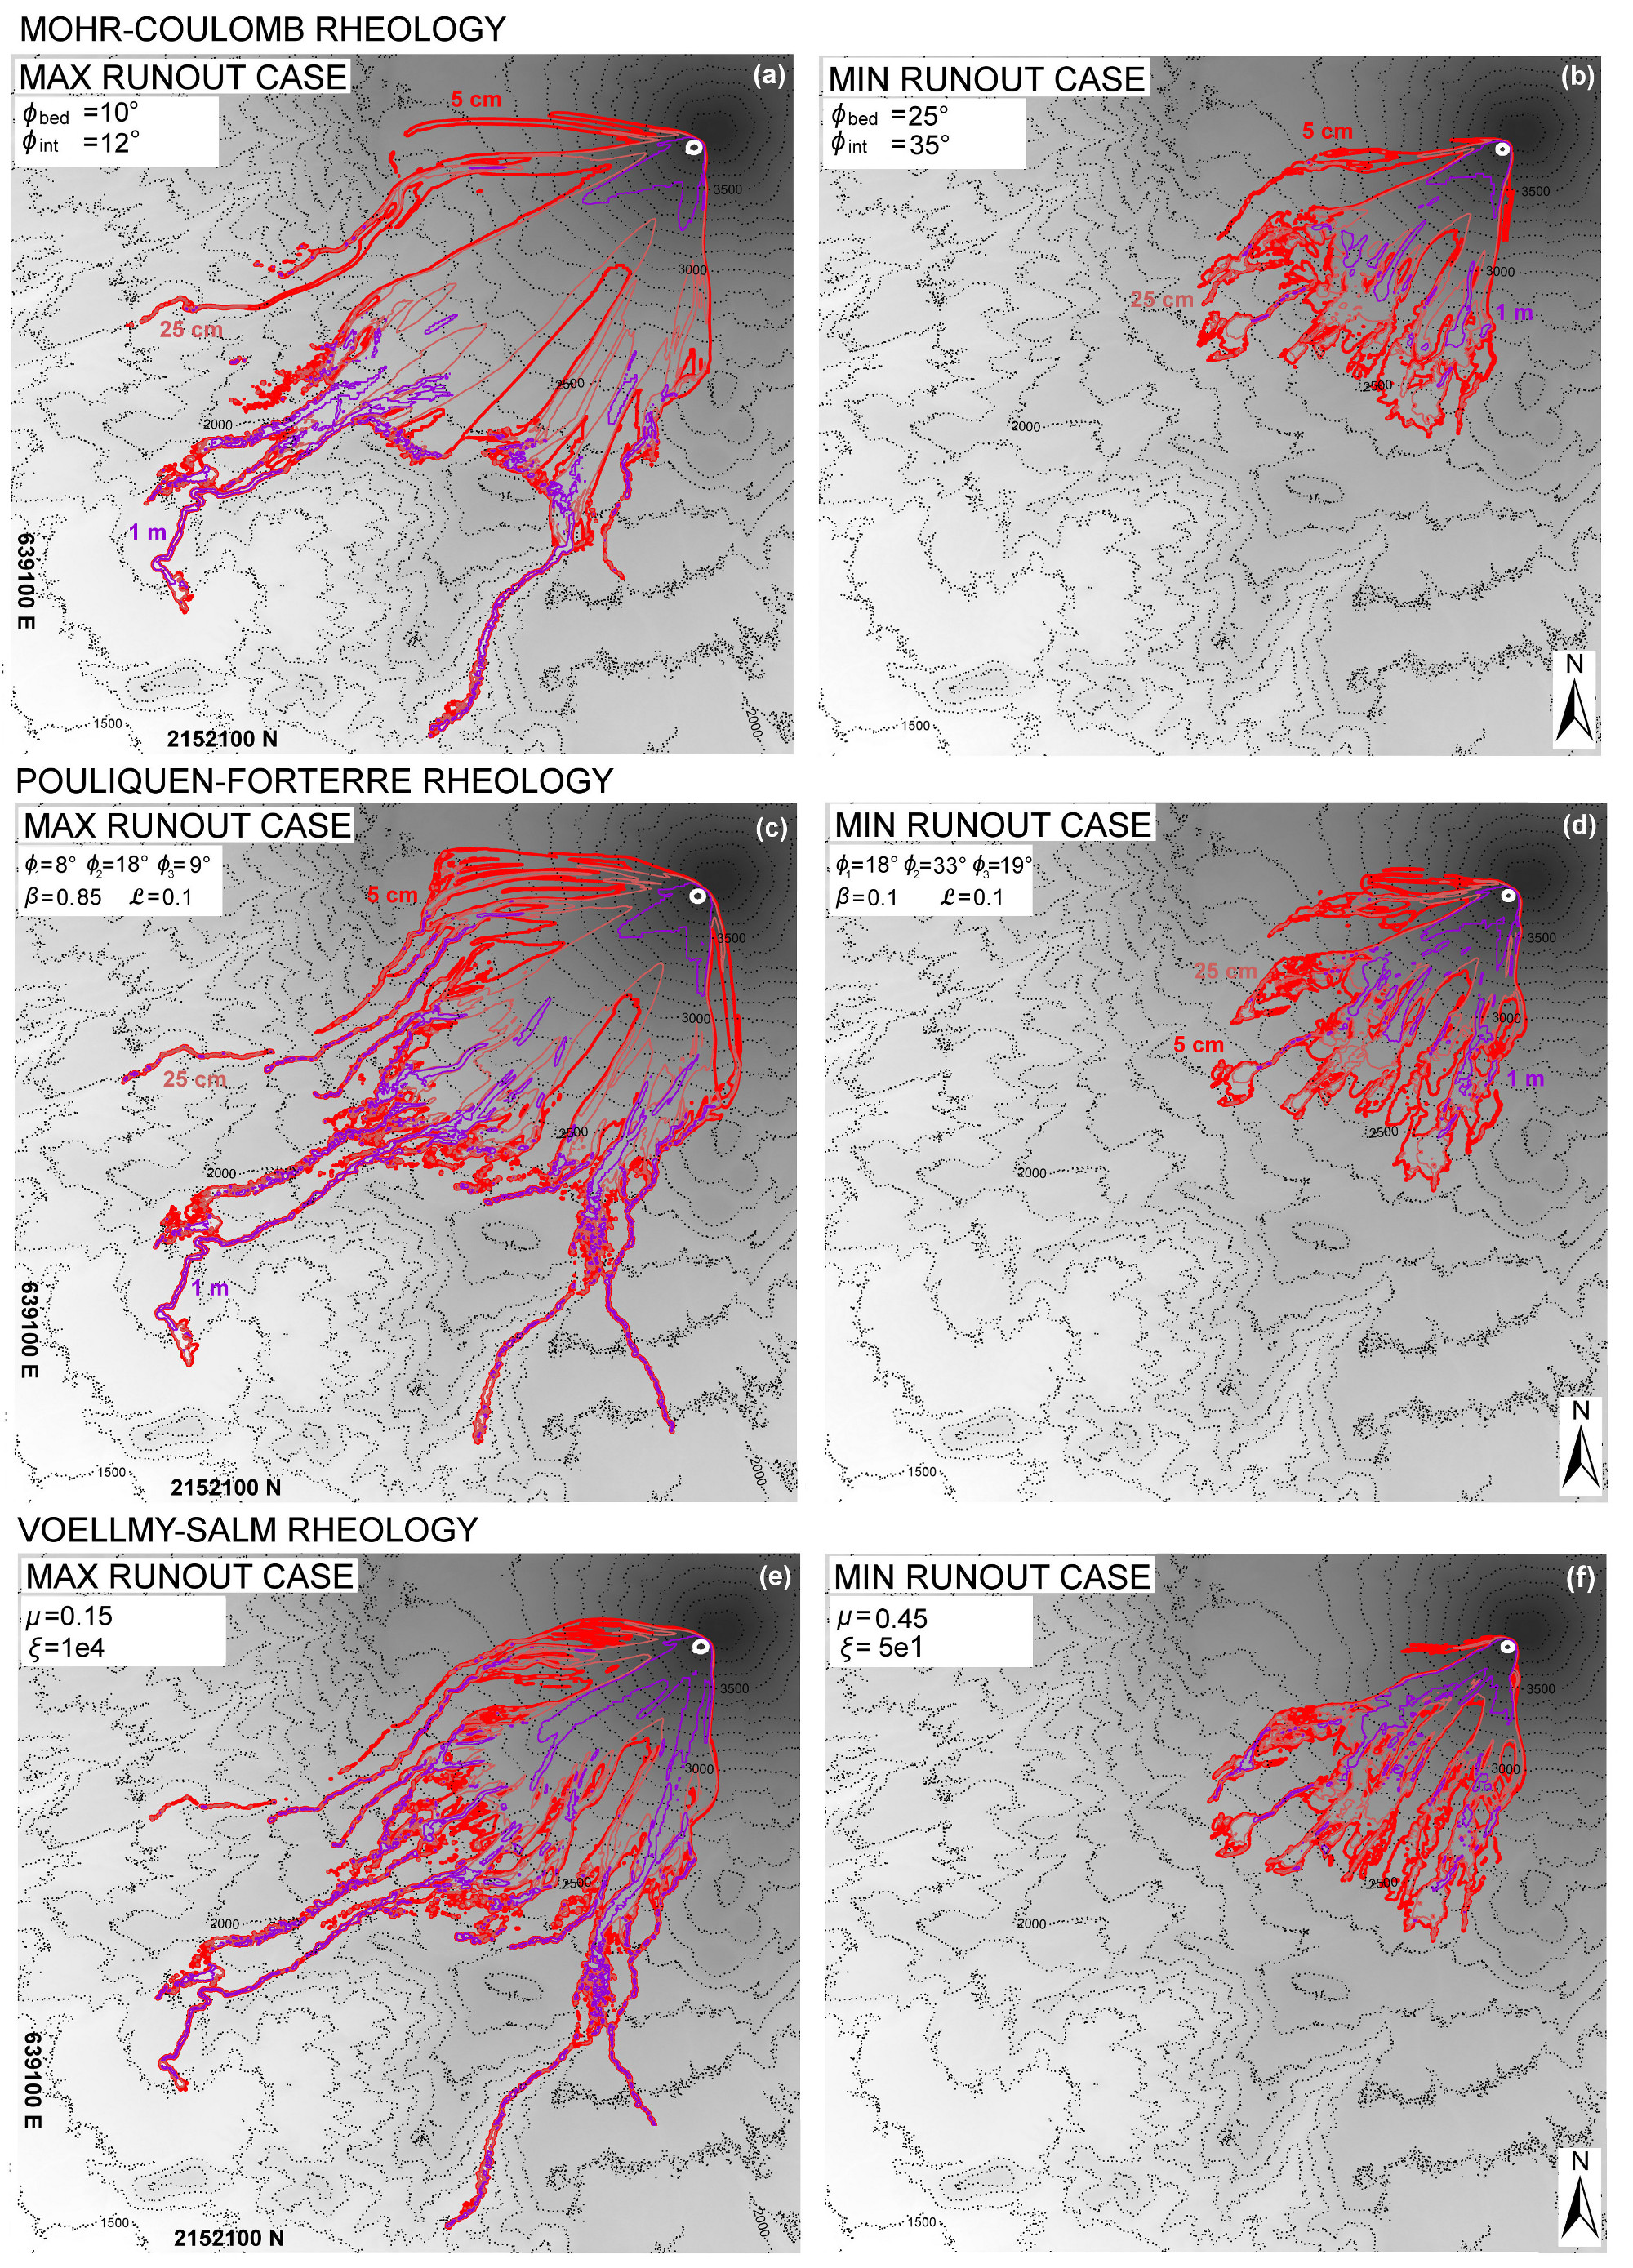
\includegraphics[width=0.85\textwidth]{Figures/ExtremeMaps.jpg}
        \caption{Volc\'an de Colima - comparison between \emph{max flow height} maps of simulated flow, assuming MC (a),(d), PF (b),(e), and VS (c),(f) models. Extreme cases - (a),(b),(c) \emph{\textbf{max. volume -- min. resistance}} and (d),(e),(f) \emph{\textbf{min. volume -- max. resistance}}.}
        \label{Colima-MaxMinExtents}
\end{figure}
Figure \ref{Colima-MaxMinExtents} displays the maps of maximum flow height observed in the extreme cases tested. Simulation options are - max\_time = 7200 s (2 hours), height/radius = 0.55, length\_scale = 4e3 m, number\_of\_cells\_across\_axis = 50, order = first, geoflow\_tiny = 1e4 \citep{Patra2005,Aghakhani2016}. Initial pile geometry is paraboloid.
\newpage
\begin{itemize}
\item \textbf{Material Volume:} $[2.08, 3.12] \times 10^5 \ m^3$, i.e. average of $2.6  \times 10^5 \ m^3$ and uncertainty of $\pm 20\%$.
\item \textbf{Rheology models' parameters:}
\par\noindent \textbf{MC} - $\phi_{bed} \in [10^{\mathrm{\circ}}, 25^{\mathrm{\circ}}]$.

\vskip.1cm\noindent \textbf{PF} - $\phi_1 \in [8^{\mathrm{\circ}}, 18^{\mathrm{\circ}}]$.

\vskip.1cm\noindent \textbf{VS} - $\mu \in [0.15, 0.45]$, $\quad \log(\xi) \in [1.7, 4]$.

\end{itemize}

The models display different macroscopic features. In particular, VS lateral spreading is significant lower and the material reaches higher thickness, whereas PF model seems to stop more gradually than MC with more complex inundated area boundary lines. These features are consequence of the different assumptions constituting the models.

\subsection{Flow height in 51 locations - Mohr-Coulomb model}
The number of spatial locations is significantly high. We placed 51 points to span the entire inundated area, in search of different flow regimes, as displayed in Fig. \ref{fig:Colima-first}. We remark that all the distances reported in the following are obtained by projection on the vertical axis, without considering the differences in elevation.
\begin{figure}[H]
         \centering
        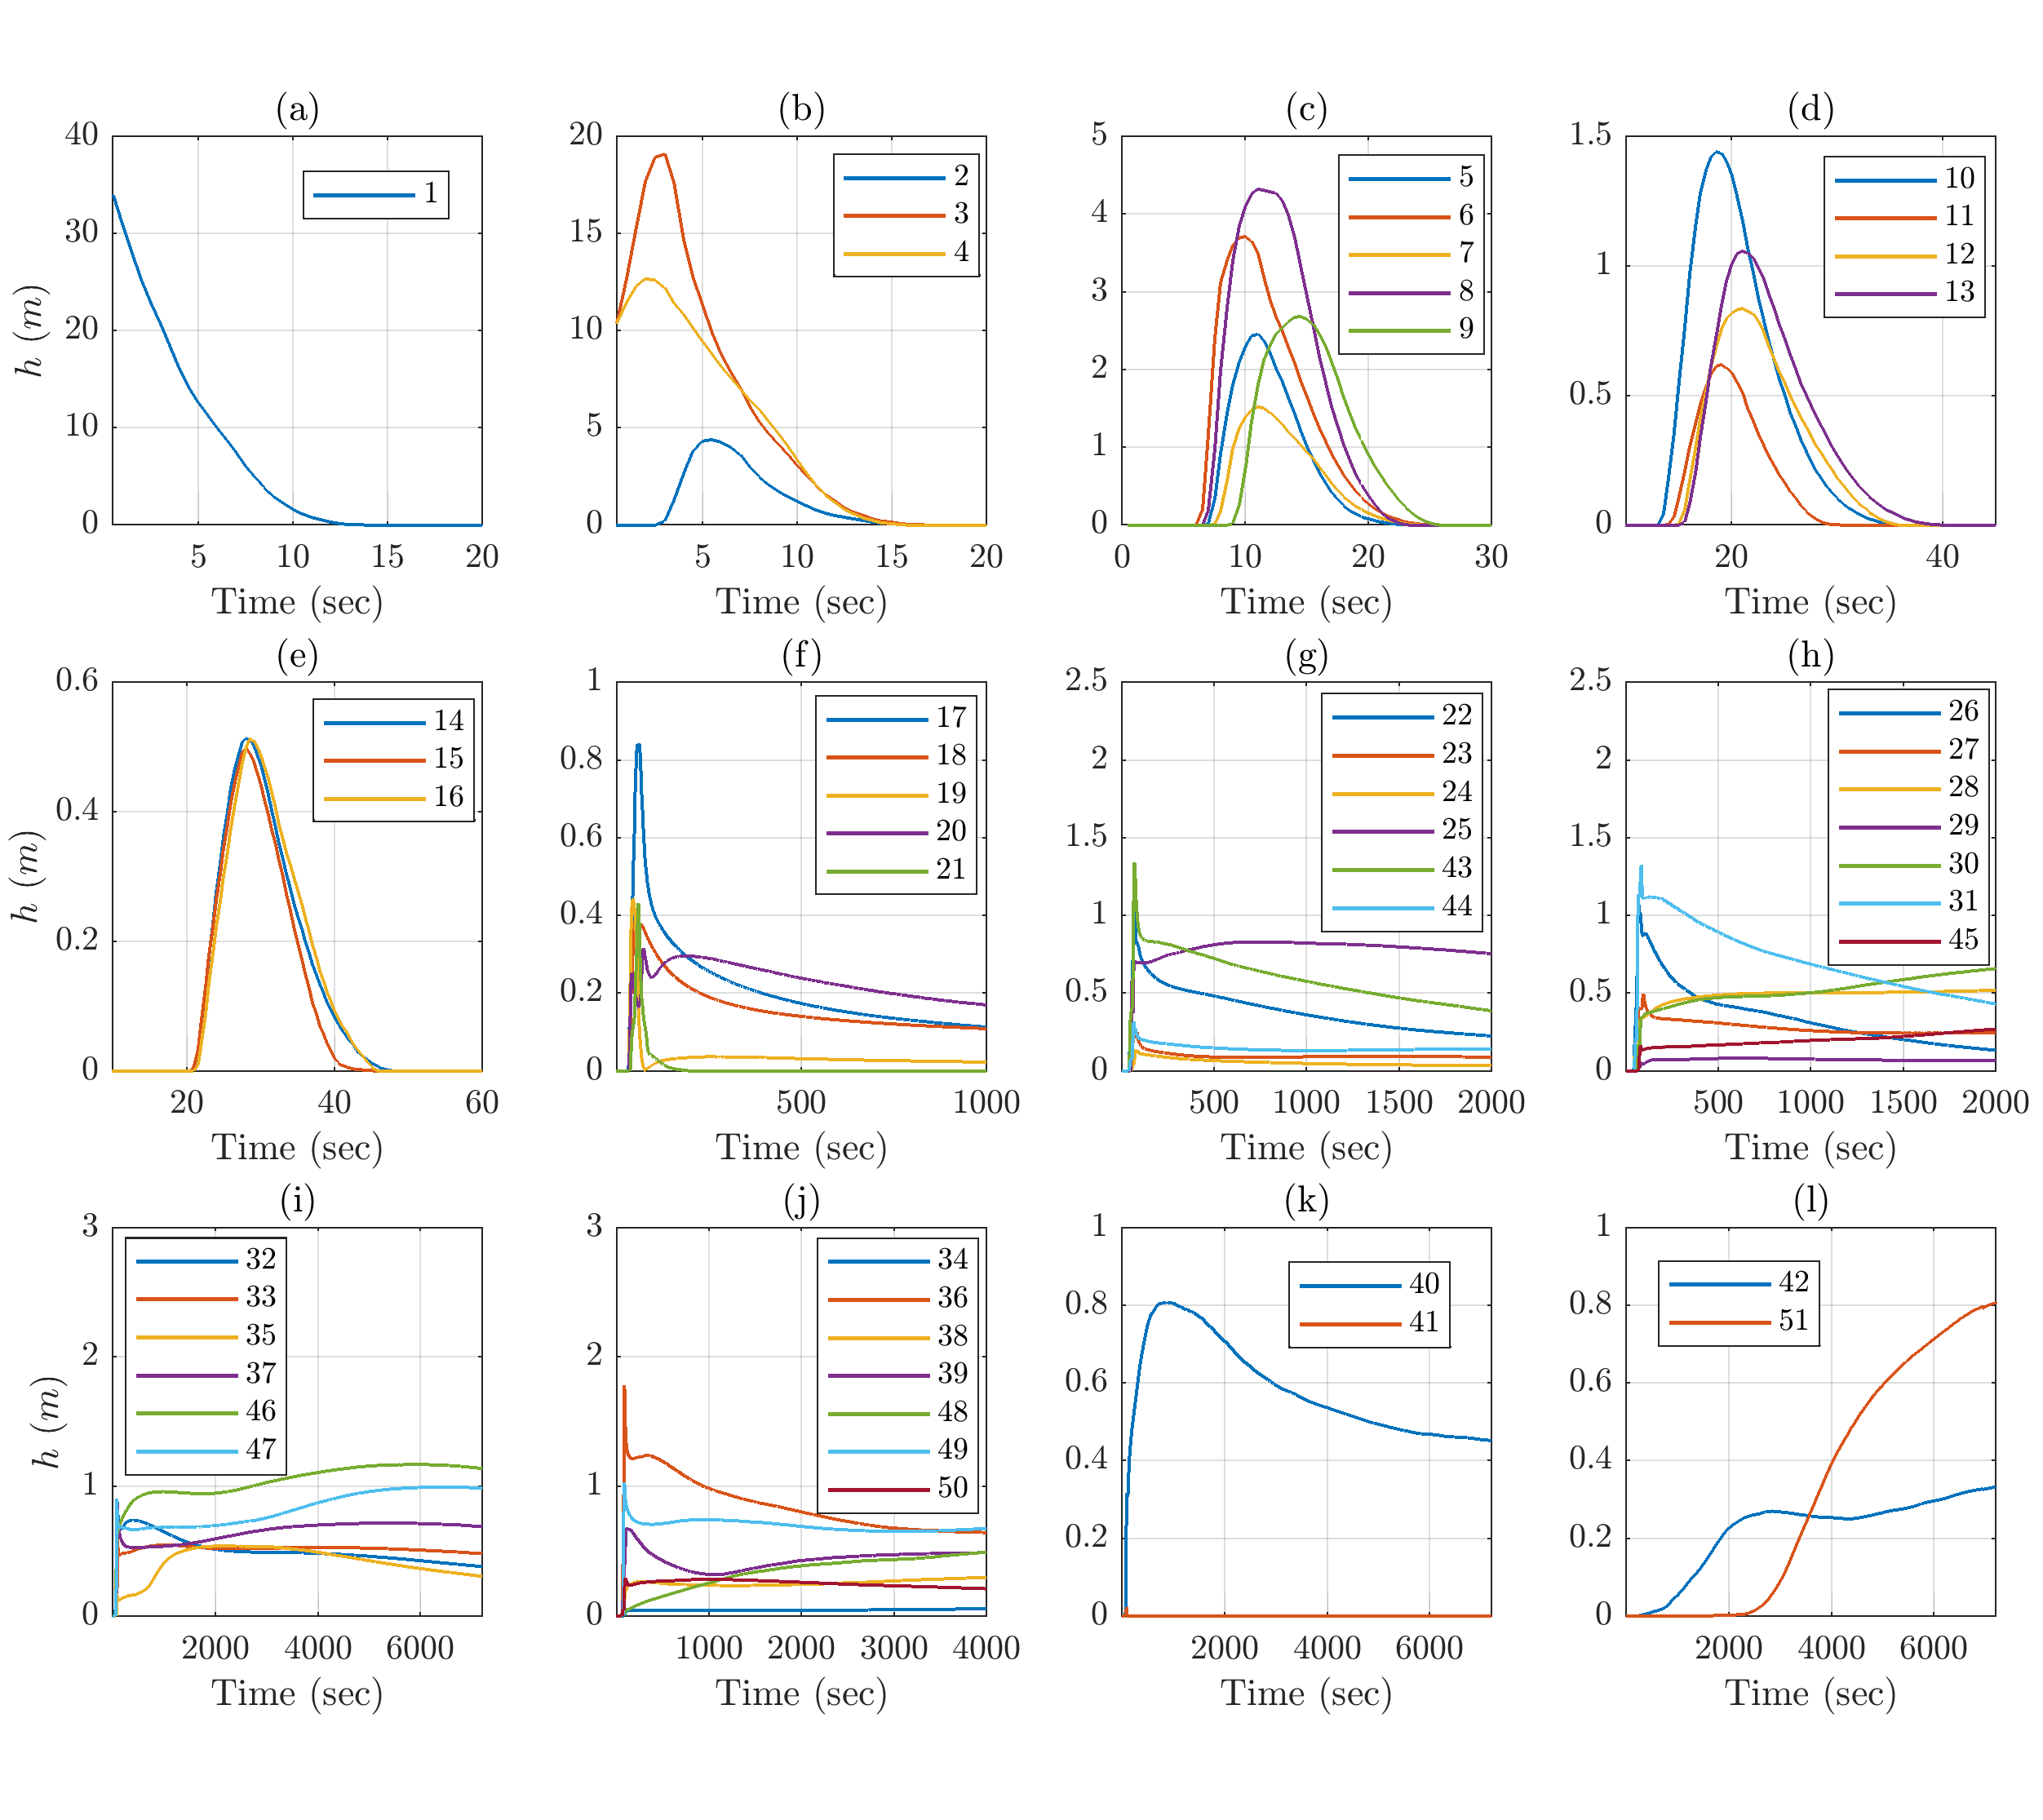
\includegraphics[width=0.9\textwidth]{MC&VS_51/Height_MC2.png}
        \caption{MC model, records of average flow height, $h(L,t)$, in 51 spatial locations of interest (Fig. \ref{fig:Colima-first}).}
        \label{fig:BAF-H-MC}
\end{figure}
Figure \ref{fig:BAF-H-MC} shows the mean flow height, $h(L,t)$, at the 51 spatial locations of interest, according to MC. Different plots have different scales on either time and space axes. In plot \ref{fig:BAF-H-MC}a, the only location is set on the center of the initial pile, and the profile is similar to what observed in point $L_1$ of the inclined plane case study, in Fig.\ref{fig:Ramp-H}a. In this case the height decreases from the initial value to zero in $\sim 15 s$. In plots \ref{fig:BAF-H-MC}b,c,d,e, the locations are are set at less than $\sim 1$ km radius from the initial pile. Their profiles are similar to point $L_2$ in Fig.\ref{fig:Ramp-H}b. The height profile is bell-shaped, starting from zero and then waning back to zero in $\sim 20$ s. All the dynamics occurs during the first minute. In plots \ref{fig:BAF-H-MC}f,g,h,i,j, points are set where the slope reduces, and the flow can channelize, and typically leaves a deposit. The distance from the initial pile is $\sim 2-3$ km. The profiles are sometimes similar to $L_3$ of Fig.\ref{fig:Ramp-H}c, other times to $L_4$ of Fig.\ref{fig:Ramp-H}d, in a few cases showing intermediate aspects. In general is either observed an initial short-lasting bulge followed by a slow decrease lasting for several minutes and asymptotically tending to a positive height, or a steady increase of material height tending to a positive height. In both cases it is sometimes observed a bimodal profile in the first 5 minutes. Finally, plots \ref{fig:BAF-H-MC}k,l focus on three points set at about the runout distance of the flow, in the most important ravines, at $\sim 4-5$ km from the initial pile. Profiles are similar to what observed in point $L_4$ of Fig.\ref{fig:Ramp-H}d. Plots of the Froude Number at the 51 points are included in Supporting Information S3 - strongly bimodal profiles and sharp changes are observed due to the interplay between flow height and flow speed.

\subsection{Observable outputs - UQ in 6 selected locations}\label{Obs2}
The six selected locations are $[L_8, L_{10}, L_{17}, L_{39}, L_{43}, L_{46}]$, as displayed in Figure \ref{fig:Colima-extra}). The first two points, $L_8$ and $L_{10}$, are both proximal to the initiation pile. Points $L_{17}$ and $L_{43}$ are placed where the slope is reducing and the ravine channels start, and $L_{39}$ and $L_{46}$ are placed in the channels, further down-slope. Moreover, $L_8$, $L_{43}$, and $L_{46}$ are placed at the western side of the inundated area, whereas $L_{10}$, $L_{17}$, and $L_{39}$ are placed at the eastern side.
\begin{figure}[H]
         \centering
        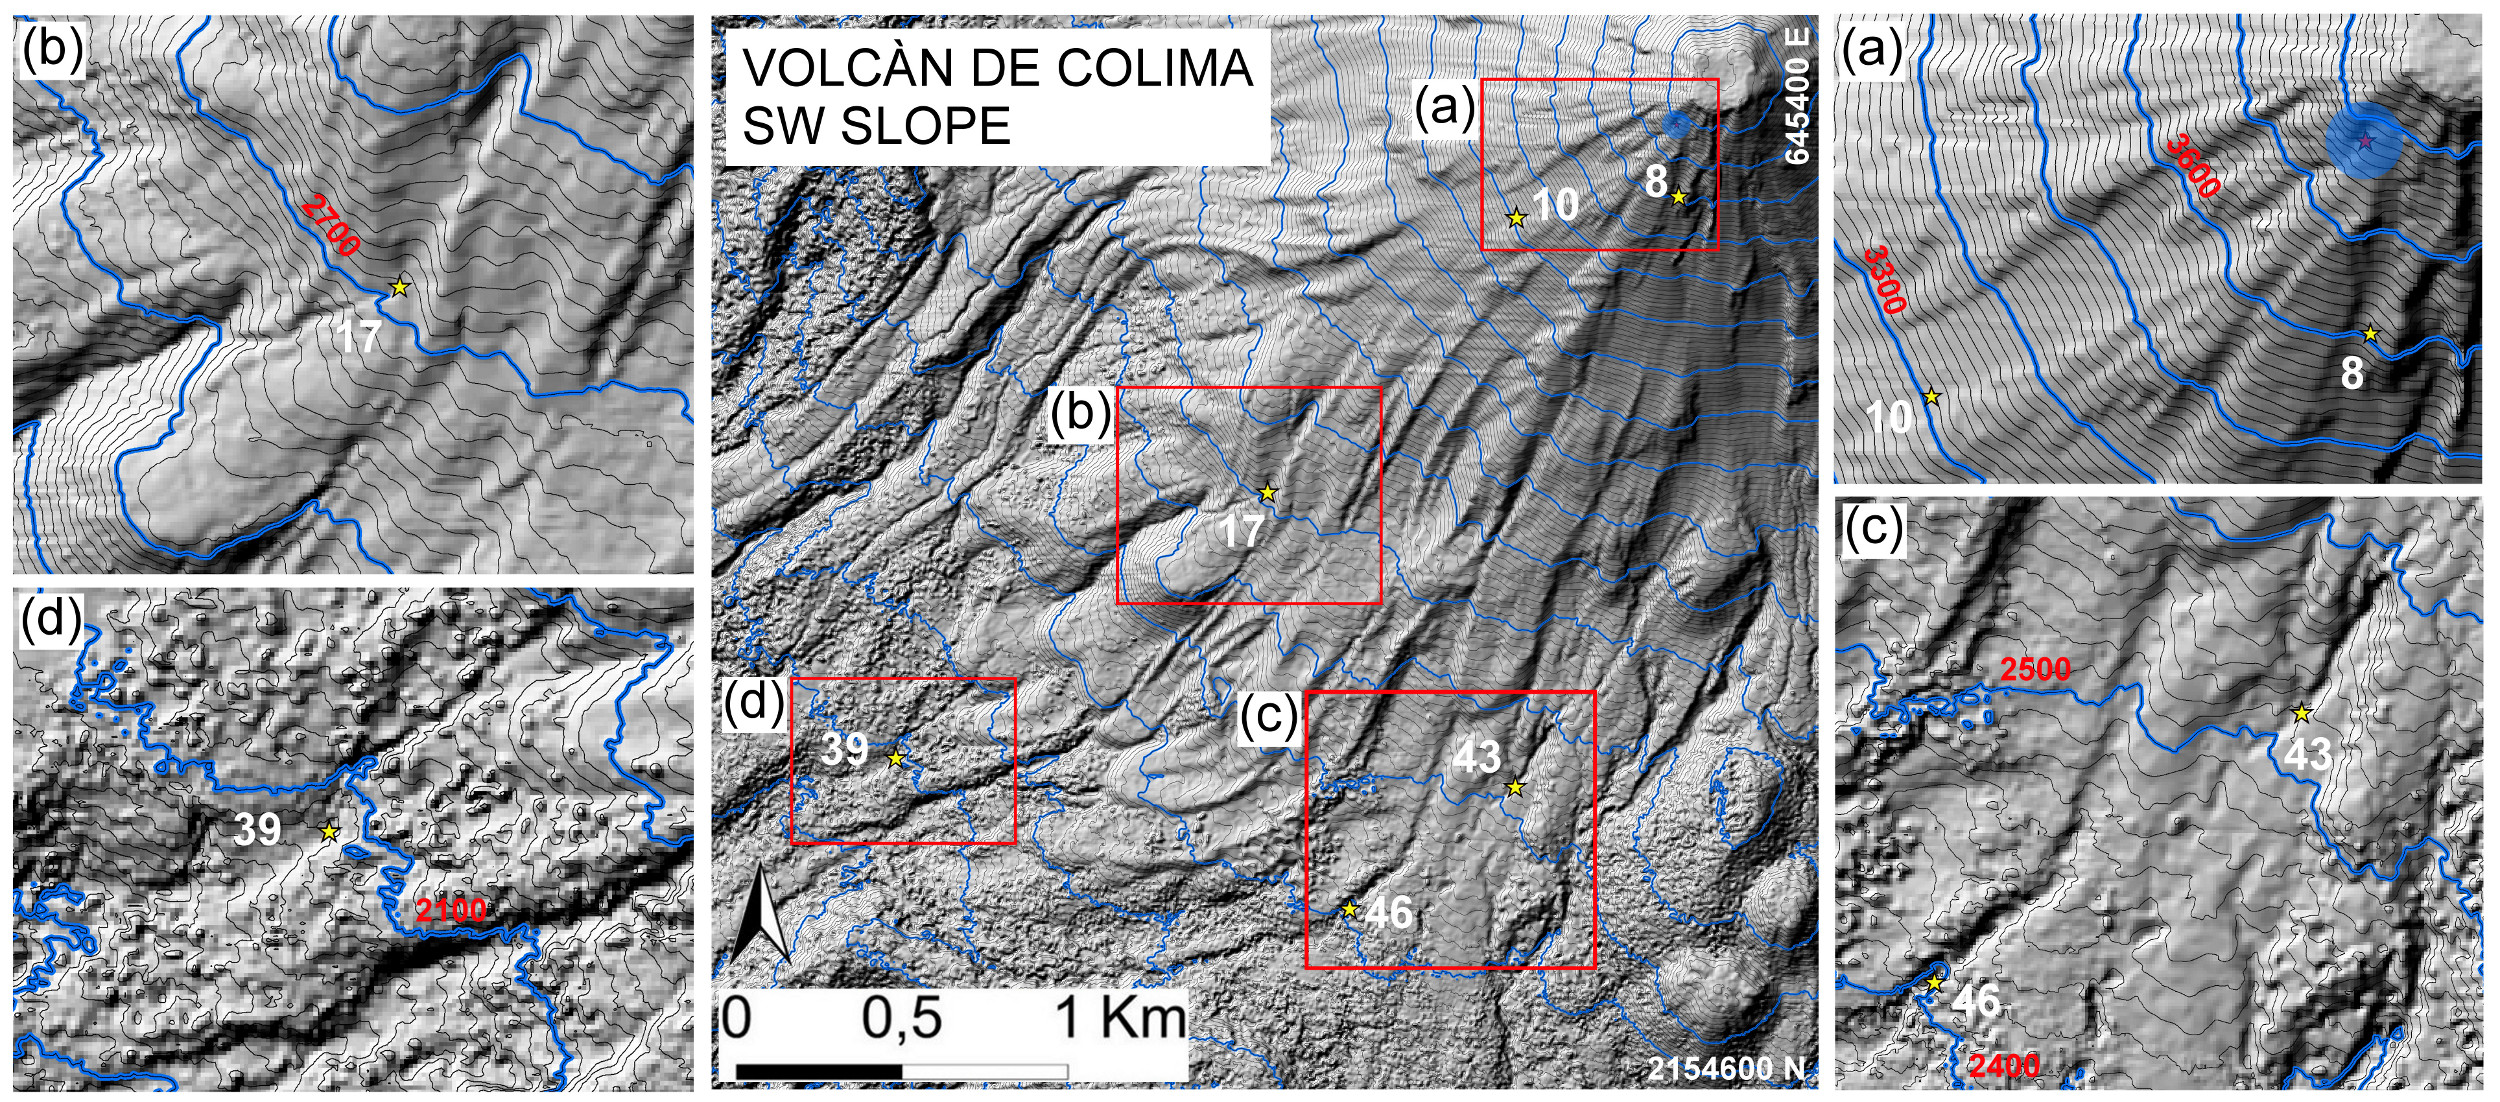
\includegraphics[width=1\textwidth]{BAF_VolcanDeColima/FigExtra.jpg}
        \caption{Volc{\'a}n de Colima (M{\'e}xico) overview, including six selected sample sites (stars). In (a), (b), (c), (d) are enlarged the topographic features in proximity of those locations. Pile location is marked by a blue dot. Reported coordinates are in UTM zone 13N. Elevation isolines are included, at intervals of $10 m$ in black, and $100m$ in bold blue. Elevation values in red.}
        \label{fig:Colima-extra}
\end{figure}

\subsubsection{Flow height}
Figure \ref{fig:Colima-H} shows the flow height, $h(L,t)$, at the points $(L_i)_{i=8,10,17,39,43,46}$. Locally measured Froude Number and flow acceleration are included in Supporting Information S4 and S5. Distances from the initial pile are vertically projected.
\begin{figure}[H]
         \centering
        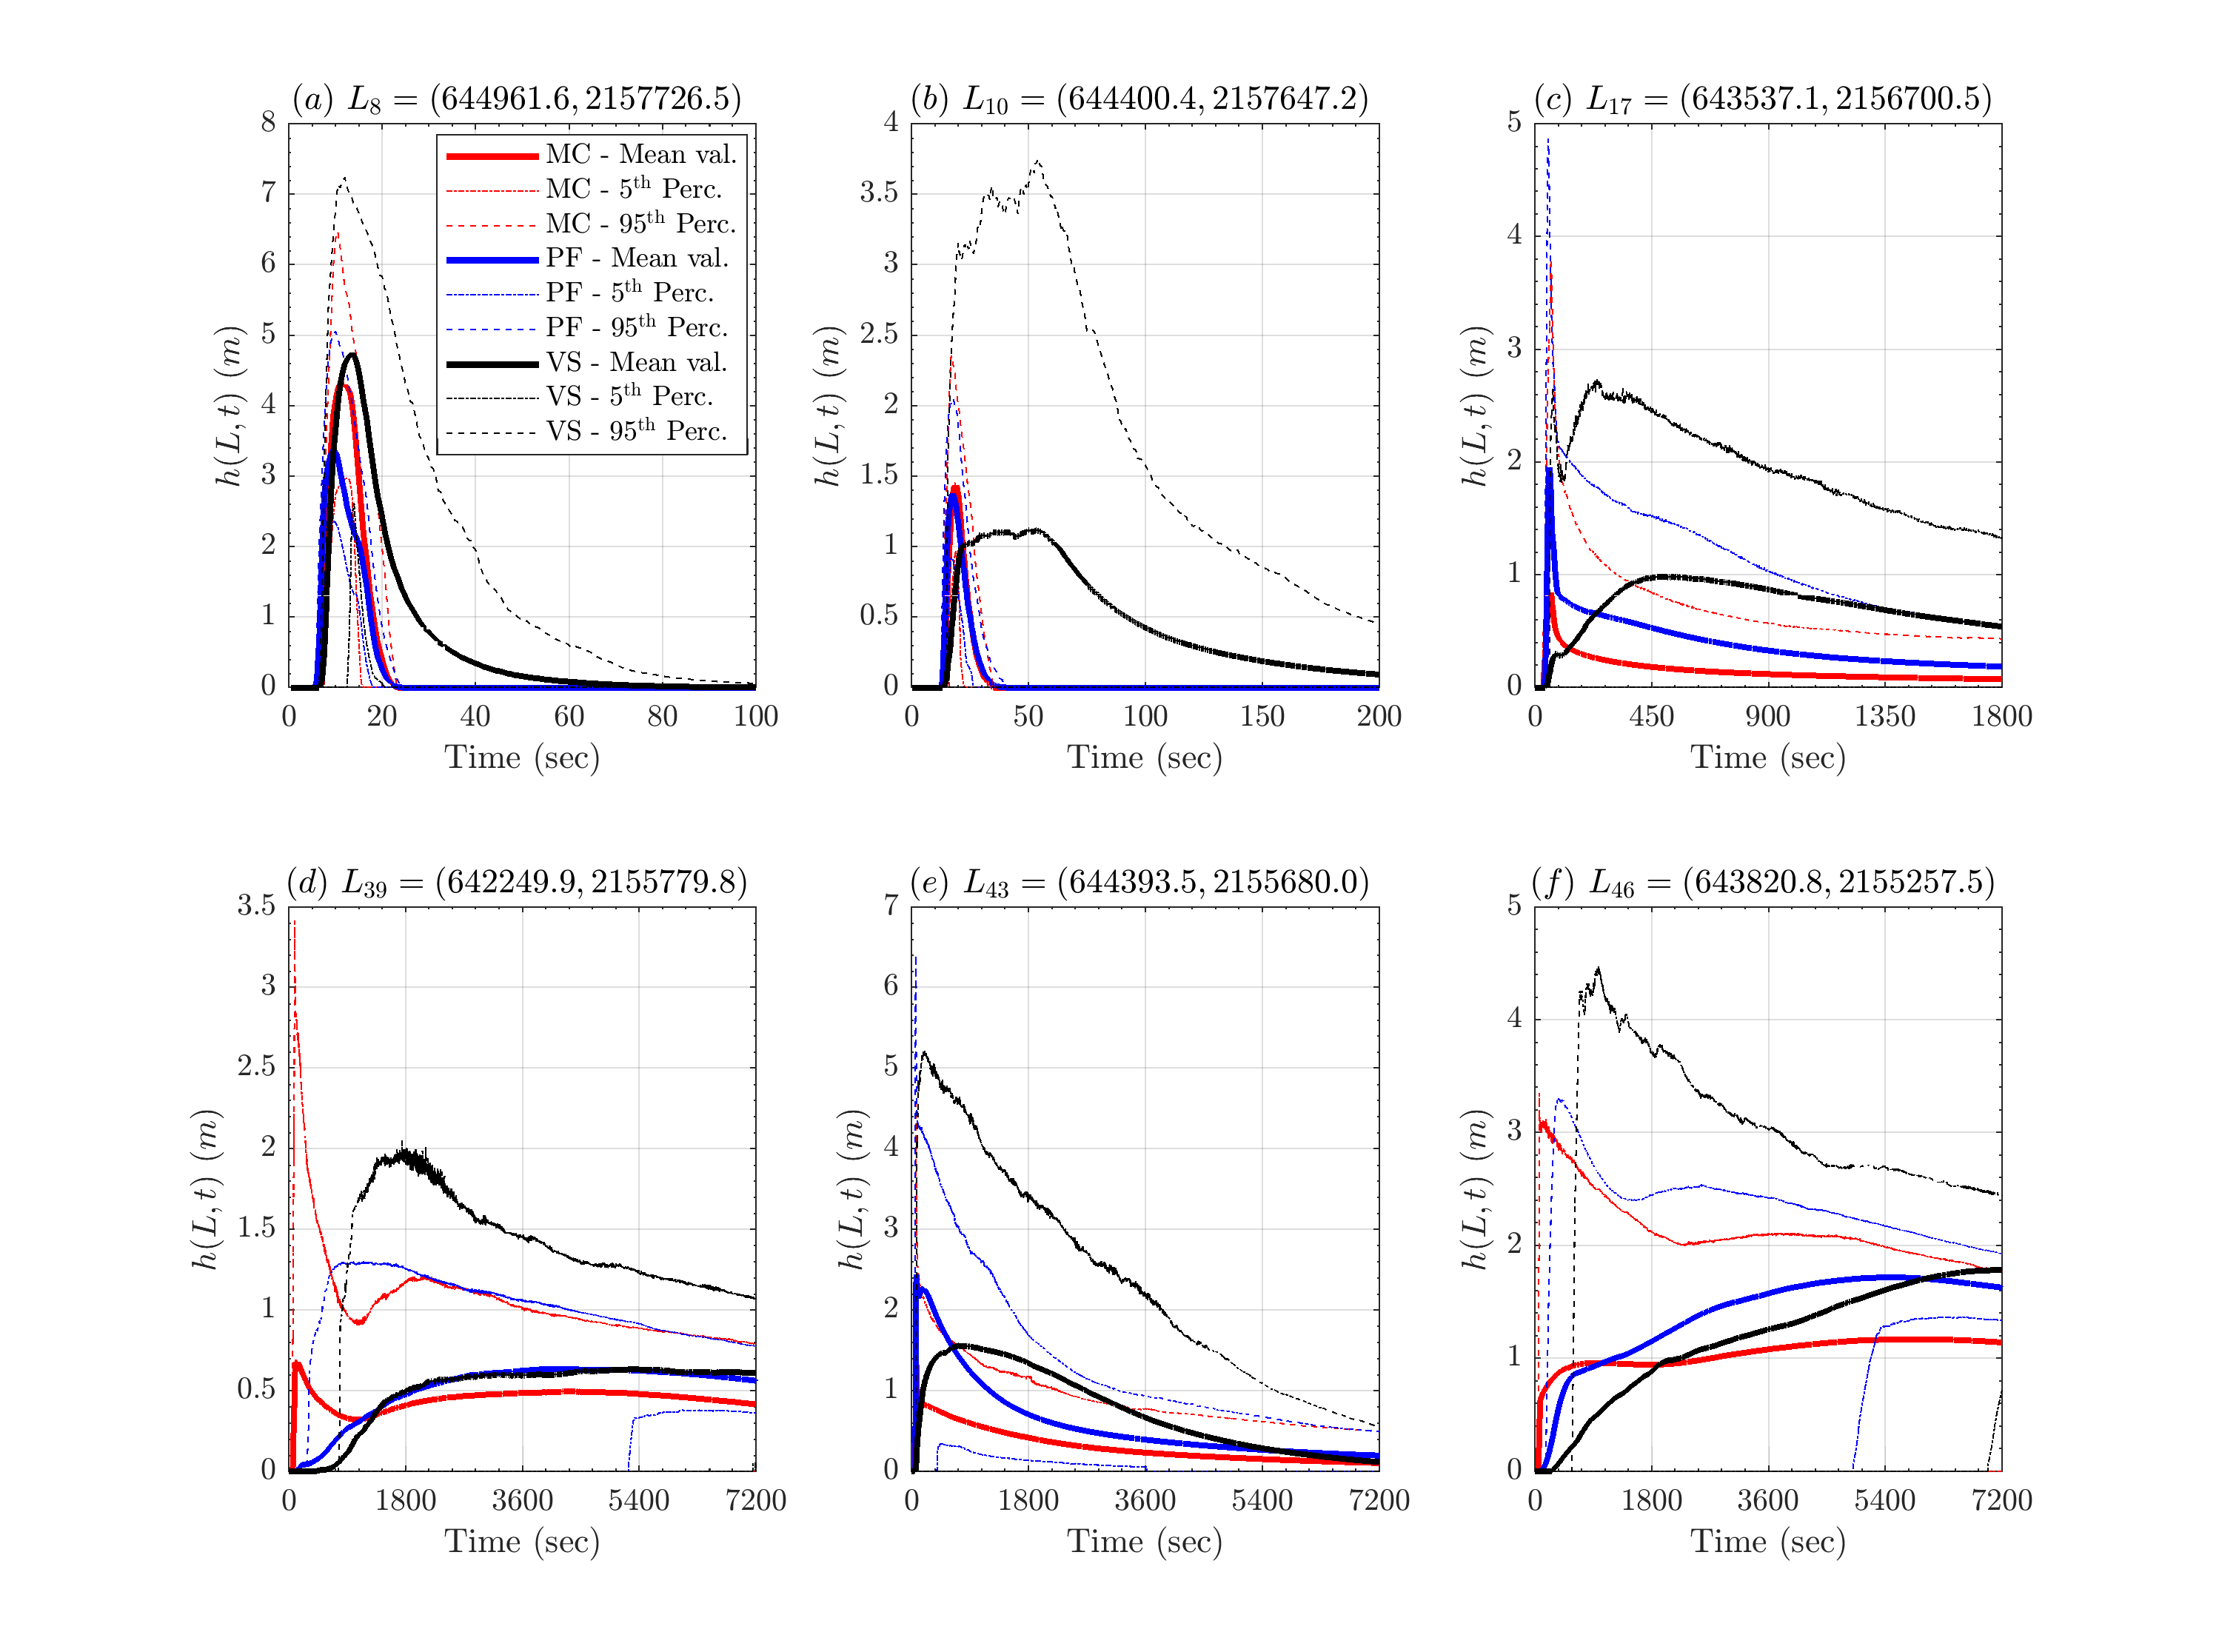
\includegraphics[width=1\textwidth]{BAF_VolcanDeColima/LocalMeasurments/Height.png}
        \caption{Records of flow height at six selected locations. Bold line is mean value, dashed/dotted lines are 5$^{\mathrm{th}}$ and 95$^{\mathrm{th}}$ percentile bounds. Different models are displayed with different colors. Plots are at different scale, for simplifying lecture.}
        \label{fig:Colima-H}
\end{figure}
In plots \ref{fig:Colima-H}a,b, we show the flow height in points $L_8$ and $L_{10}$, $\sim 200 m$ and $\sim 500 m$ from the initial pile, respectively. $L_8$ is on the east side, and $L_{10}$ on the west side of the flow. Models MC and PF display similar profiles, positive for less than $15 s$ and bell-shaped. VS requires a significantly longer time to decrease, particularly in point $L_{10}$, where the average flow height is still positive after $\sim 200 s$. Peak average values in $L_8$ are $3.4 m$ in $PF$, $4.3 m$ in MC, $4.7 m$ in VS. Uncertainty is $\sim \pm 2 m$, halved on the lower side in $MC$, and $PF$. In $L_{10}$, models MC and PF are almost indistinguishable, with peak height at $1.4 m$ and uncertainty $\pm 0.5 m$. Model VS, in contrast, has a maximum height of $1.1 m$ lasting for $50s$, and 95$^{th}$ percentile reaching $3.7 m$. In plots \ref{fig:Colima-H}c,e, we show the flow height in points $L_{17}$ and $L_{43}$, both at $\sim 2 km$ from the initial pile, on the west and east side of the flow, respectively. All the three models show in both the points a fast spike during the first minute, followed by a slow decrease, still showing a positive average height after 30 minutes. Again, VS is significantly different from MC and PF, and has a secondary rise peaking at $\sim 450 s$, which is not observed in the other models. This produces higher values for the most of the temporal duration, but converges to similar deposit thickness after more than 1 hour. Maximum values are $1 m$ for MC, $2 m$ for PF, and $1.5 m$ for VS, in both locations. The 5$^{th}$ percentile is zero in all the models, meaning that the parameter range does not always allow the flow to reach those locations. The 95$^{th}$ percentile is always above $5m$ in the models, except in VS, point $L_{17}$. In plots \ref{fig:Colima-H}d,f, we show the flow height in points $L_{39}$ and $L_{46}$, both placed at more than $3 km$ from the initial pile, on the west and east side of the flow, respectively. The three models all show an increasing profile, except in MC, in point $L_{39}$, which display an initial spike and a decrease before to rise again. A similar decreasing profile can be also observed in the 95$^{th}$ percentiles of all the models. It is significant that the 5$^{th}$ percentile of PF becomes positive after $\sim 5400 s$, meaning that the flow almost surely has reached that location. Deposit thickness is $\sim 0.5 m$ in all the models in point $L_{39}$, and $1.7 m$ in VS, $1.6 m$ in PF, $1.2 m$ in MC, in $L_{46}$.

\subsection{Statistical analysis of latent variables}\label{Hq2}
Figure \ref{fig:Colima-Pr1} shows the Dominance Factors $(P_i)_{i=1,\dots,4}$ of the RHS terms modulus, in the three selected proximal points $L_{8}$, $L_{10}$, and $L_{17}$, closer than 1 km to the initial pile.
\begin{figure}[H]
         \centering
        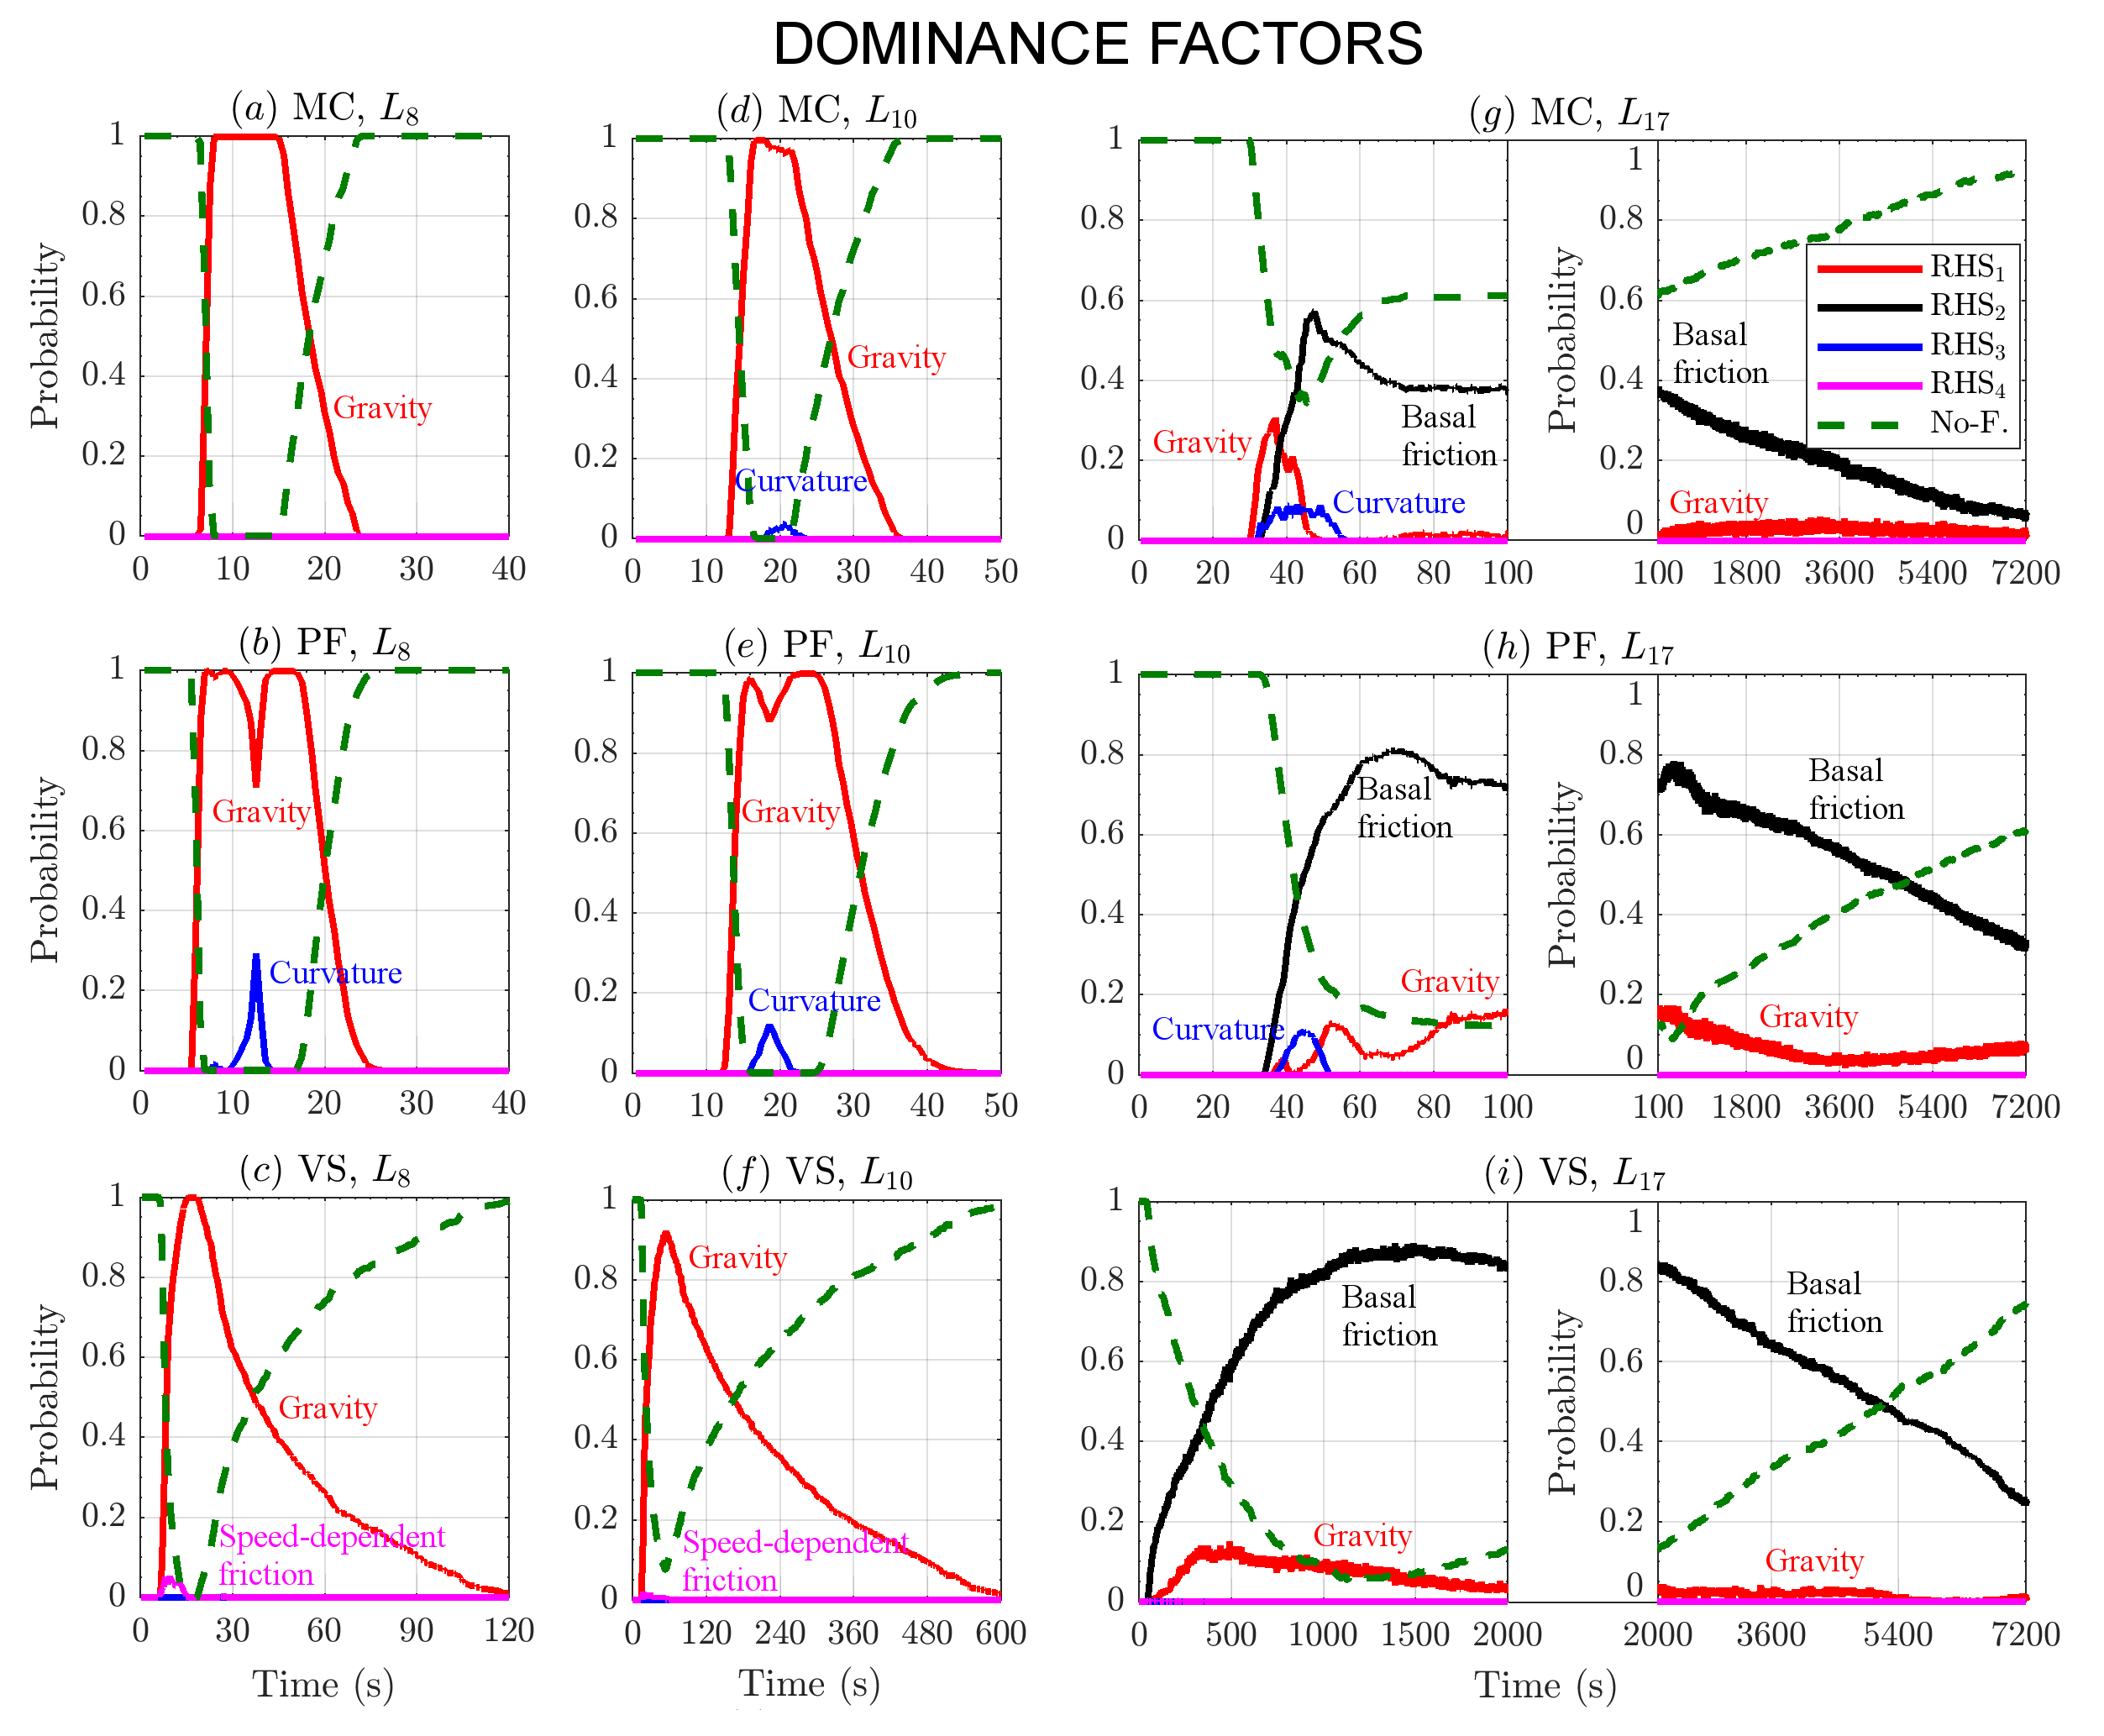
\includegraphics[width=0.95\textwidth]{BAF_VolcanDeColima/ForceContrib/Pr1_total.png}
        \caption{Records of dominance probabilities of \textbf{RHS} force moduli, at three spatial locations of interest in the first km of runout. Different models are displayed with different colors. No-flow probability is displayed with a green dashed line.}
        \label{fig:Colima-Pr1}
\end{figure}
The plots \ref{fig:Colima-Pr1}a,b,c and \ref{fig:Colima-Pr1}d,e,f are related to point $L_8$ and $L_{10}$, respectively. They are significantly similar. $\boldsymbol{RHS_1}$ related to the gravitational force is the dominant force with a very high chance, $P_1>90\%$. In MC and PF there is a small probability, $P_3=5\%-30\%$, of $\boldsymbol{RHS_3}$ being the dominant force for $\sim 5 s$. In VS it is observed a $P_4=5\%$ chance of $\boldsymbol{RHS_4}$ being dominant, for a few seconds, anticipating the minimum of no-flow probability. Plots \ref{fig:Colima-Pr1}g,h,i, are related to point $L_{17}$, and the plots are split in two sub-frames following different temporal scales. In all the models, $\boldsymbol{RHS_2}$ is the most probable dominant force, and its dominance factor has a bell-shaped profile, similar to the complementary of no-flow probability. In all the models, $\boldsymbol{RHS_1}$ has also a small chance of being the dominant force. In MC, this is more significant, at most $P_1=30\%$ for $\sim 20 s$ after the flow arrival, and has again about $P_1=\%2$ chance to be dominant in $[100, 7200] s$. In PF, the chance is $P_1=15\%$ at most, and has two maxima, one short lasting at about $55 s$, and the second in $[100,500] s$. Also in VS, the chance is at most $P_1=15\%$, reached at $[300, 500] s$, but its profile is unimodal in time, and becomes lower than $P_1=2\%$ after $2000 s$. In MC and PF, $\boldsymbol{RHS_3}$ has a chance $P_3=10\%$ of being the dominant force at $[30, 50] s$ and $[40, 50] s$, respectively. More details about the correspondent contribution coefficients are reported in Supporting Information S6.

Figure \ref{fig:Colima-Pr2} shows the Dominance Factors $(P_i)_{i=1,\dots,4}$ in the three selected distal points $L_{39}$, $L_{43}$, and $L_{46}$, more than 2 km far away from the initial pile.
\begin{figure}[H]
         \centering
        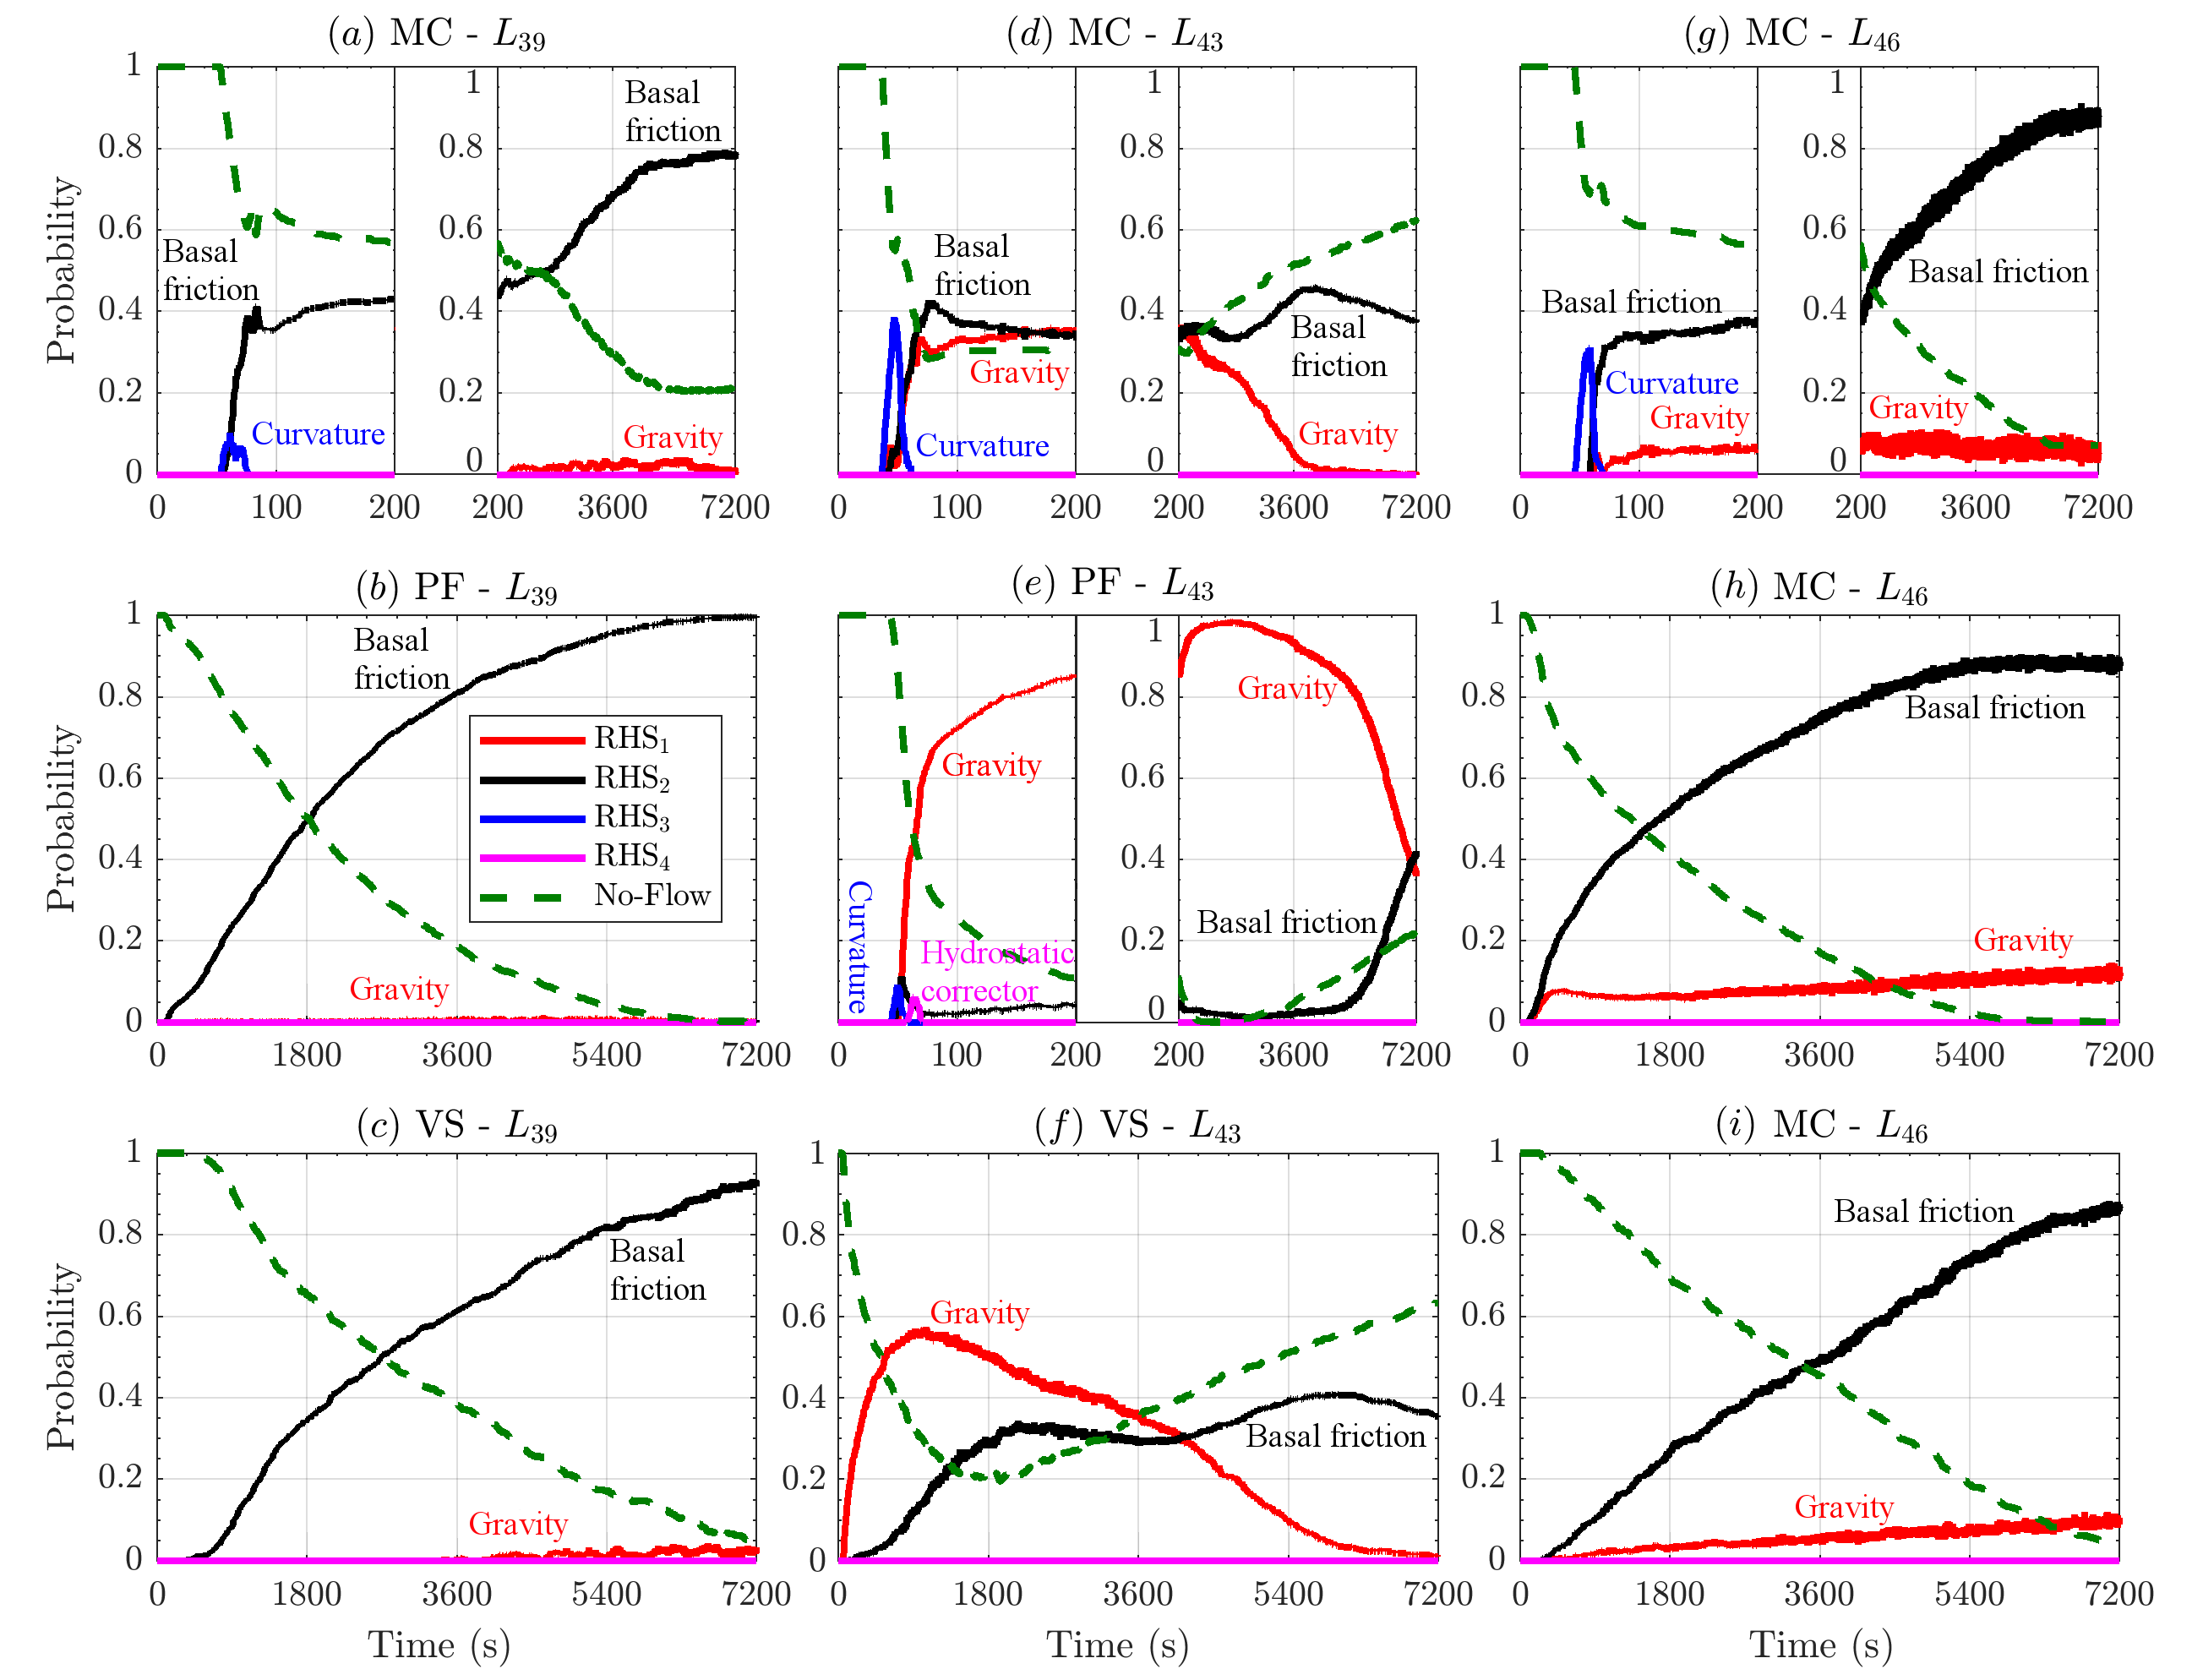
\includegraphics[width=0.95\textwidth]{BAF_VolcanDeColima/ForceContrib/Pr2_total.png}
        \caption{Records of dominance probabilities of \textbf{RHS} force modulus, at three spatial locations of interest, after 2 km of runout. Different models are displayed with different colors. No-flow probability is displayed with a green dashed line.}
        \label{fig:Colima-Pr2}
\end{figure}
The plots \ref{fig:Colima-Pr2}a,b,c and \ref{fig:Colima-Pr2}g,h,i are related to point $L_{39}$ and $L_{46}$, respectively, and they are significantly similar. These points are both in the most distal part of the ravines, on the western and eastern side of the inundated area, respectively. They are also similar to the dominance factors at point $L_{17}$, shown in plots \ref{fig:Colima-Pr1}g,h,i, but the no-flow probability never becomes negligible in this case. The probability of $\boldsymbol{RHS_2}$ being the dominant force is $P_2>90\%$ till the end of the temporal window. Moreover, $\boldsymbol{RHS_1}$ does not show any initial peak in $P_2$, and generally increases slowly, reaching a $P_2=10\%$ chance of being the dominant force in $L_{46}$, after more than $3600 s$, in all the models. Plots \ref{fig:Colima-Pr2}d,e,f, are related to point $L_{43}$, and are remarkably different. In MC, either $\boldsymbol{RHS_1}$ and $\boldsymbol{RHS_2}$ can be dominant forces, both with chances of $\sim 35\%$ in the first $200 s$. Then, $\boldsymbol{RHS_2}$ increases its chance, and becomes the only dominant force after $3600 s$. The no-flow probability is never below $30\%$. $\boldsymbol{RHS_3}$ is dominant with $P_3=35\%$ in $[40, 60] s$. In VS the no-flow probability is never below $20\%$, and the dominance factors are broadly similar to MC, although $\boldsymbol{RHS_1}$ is more relevant up to $4000 s$, and $\boldsymbol{RHS_3}$ is never dominant. Instead, in PF $\boldsymbol{RHS_1}$ is the dominant force with $P_1>90\%$ until $3600 s$, and $\boldsymbol{RHS_2}$ chance to be dominant rises only in the very last amount of time, reaching $P_2=40\%=P_1$. The no-flow probability is very low during the most of the temporal window, rising at $20\%$ only at $7200 s$. Both $\boldsymbol{RHS_3}$ and $\boldsymbol{RHS_4}$ show short peaks in the dominance factor, of about $10\%$ at $[50,60] s$.

\subsection{Flow extent and spatial integrals}
Figure \ref{fig:Colima-spatial} shows the spatial average of speed and Froude Number. It also shows the inundated area as a function of time.
\begin{figure}[H]
        \centering
        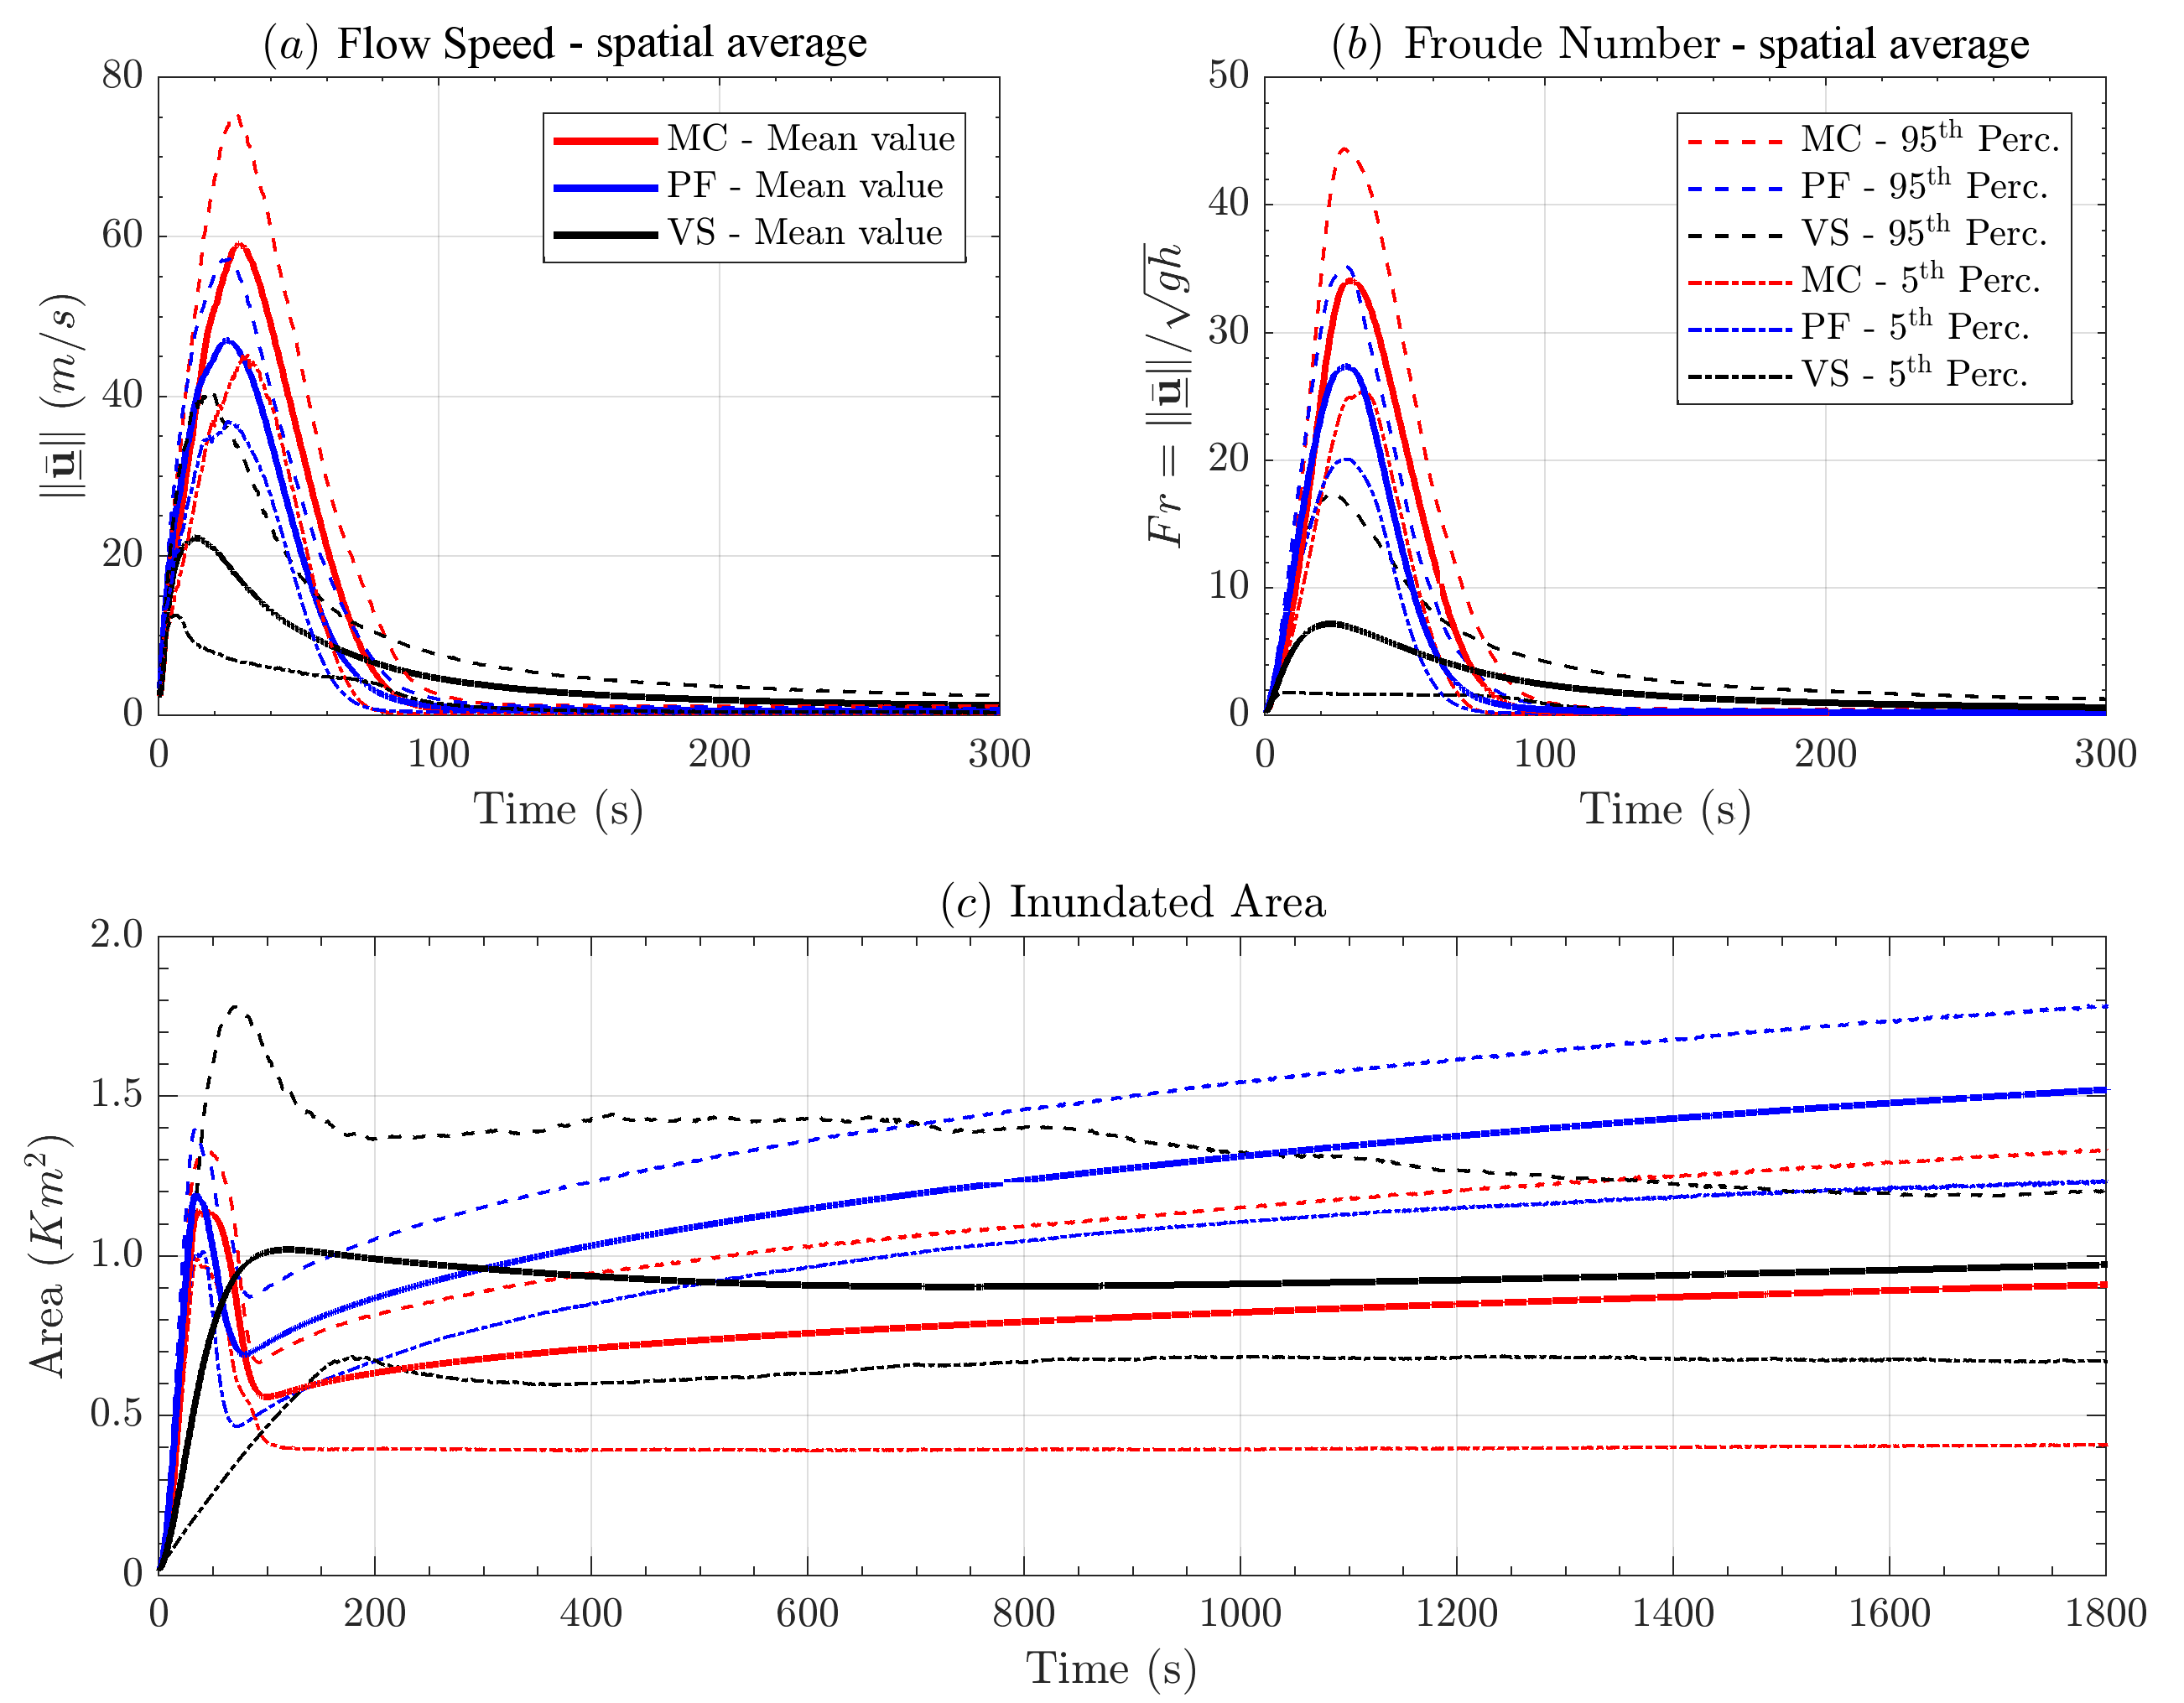
\includegraphics[width=0.85\textwidth]{BAF_VolcanDeColima/AveragedMeasurments/Averaged_MeasuresColima.png}
        \caption{Comparison between spatial averages of $(a)$ flow speed, and $(b)$ Froude Number, in addition to the $(c)$ inundated area, as a function of time. Bold line is mean value, dashed/dotted lines are 5$^{\mathrm{th}}$ and 95$^{\mathrm{th}}$ percentile bounds. Different models are displayed with different colors.}
        \label{fig:Colima-spatial}
\end{figure}
Like in Fig.\ref{fig:Ramp-spatial}, spatial averages and inundated area have smoother plots than local measurements, and most of the details observed in local measurements are not easy to discern. In plot \ref{fig:Colima-spatial}a the speed shows a bell-shaped profile in all the models, but whereas the values were significantly similar in the inclined plane experiment, in this case the maximum speed is $\sim 60 m/s$ in MC, $\sim 50 m/s$ in PF, $\sim 20 m/s$ in VS, on average. Uncertainty is $\pm 18 m/s$ in MC, similar, but skewed, in VS, and $\pm 10 m/s$ in PF. In plot \ref{fig:Colima-spatial}b, the $Fr$ profile is very similar to the speed, but the difference between VS and the other models is accentuated. Maximum values are $\sim 50$ in MC, $\sim 38$ in PF, $\sim 5$ in VS, whereas uncertainty is $\pm 10$ in MC, $\pm 7$ in PF, and skewed $[-5, +10]$ in VS. In plot \ref{fig:Colima-spatial}c, inundated area has a first peak in MC and PF, both at $\sim 1.15 km^2$, followed by a decrease to $0.55 km^2$ and $0.7 km^2$ ,respectively, and then a slower increase up to a flat plateau at $0.9 km^2$ and $1.5 km^2$, respectively. Uncertainty is $\sim \pm 0.2 km^2$ in both MC and PF until $\sim 100 s$, and then it increases at $\pm 0.3 km^2$ and $[-0.5, +0.4] km^2$, respectively. In MC this increase in uncertainty is concentrated at $\sim 100 s$, while it is more gradual in PF. VS has a different profile. The initial peak is only significant in the 95$^{th}$ percentile values, and occurs twice later, i.e. at $\sim 100 s$. The peak is of $\sim 1 km^2$ on the average, but up to $\sim 1.8 km^2$ in the 95$^{th}$ percentile. The decrease after the peak is very slow and the average inundated area is never below $0.85 km^2$, and eventually reaches back to $\sim 1 km^2$. Uncertainty is $[-0.3, +0.2] km^2$.

\subsubsection{Power integrals}
Figure \ref{fig:Colima-Power-spatial} shows the spatial sum of the powers. The estimates in this section assume the material density of the flow $\rho = 1800 kg/m^3$. This a fixed scaling factor, and the plots aspect is not affected by its value. Corresponding plots of the force terms are included in Supporting Information S7.
\begin{figure}[H]
        \centering
        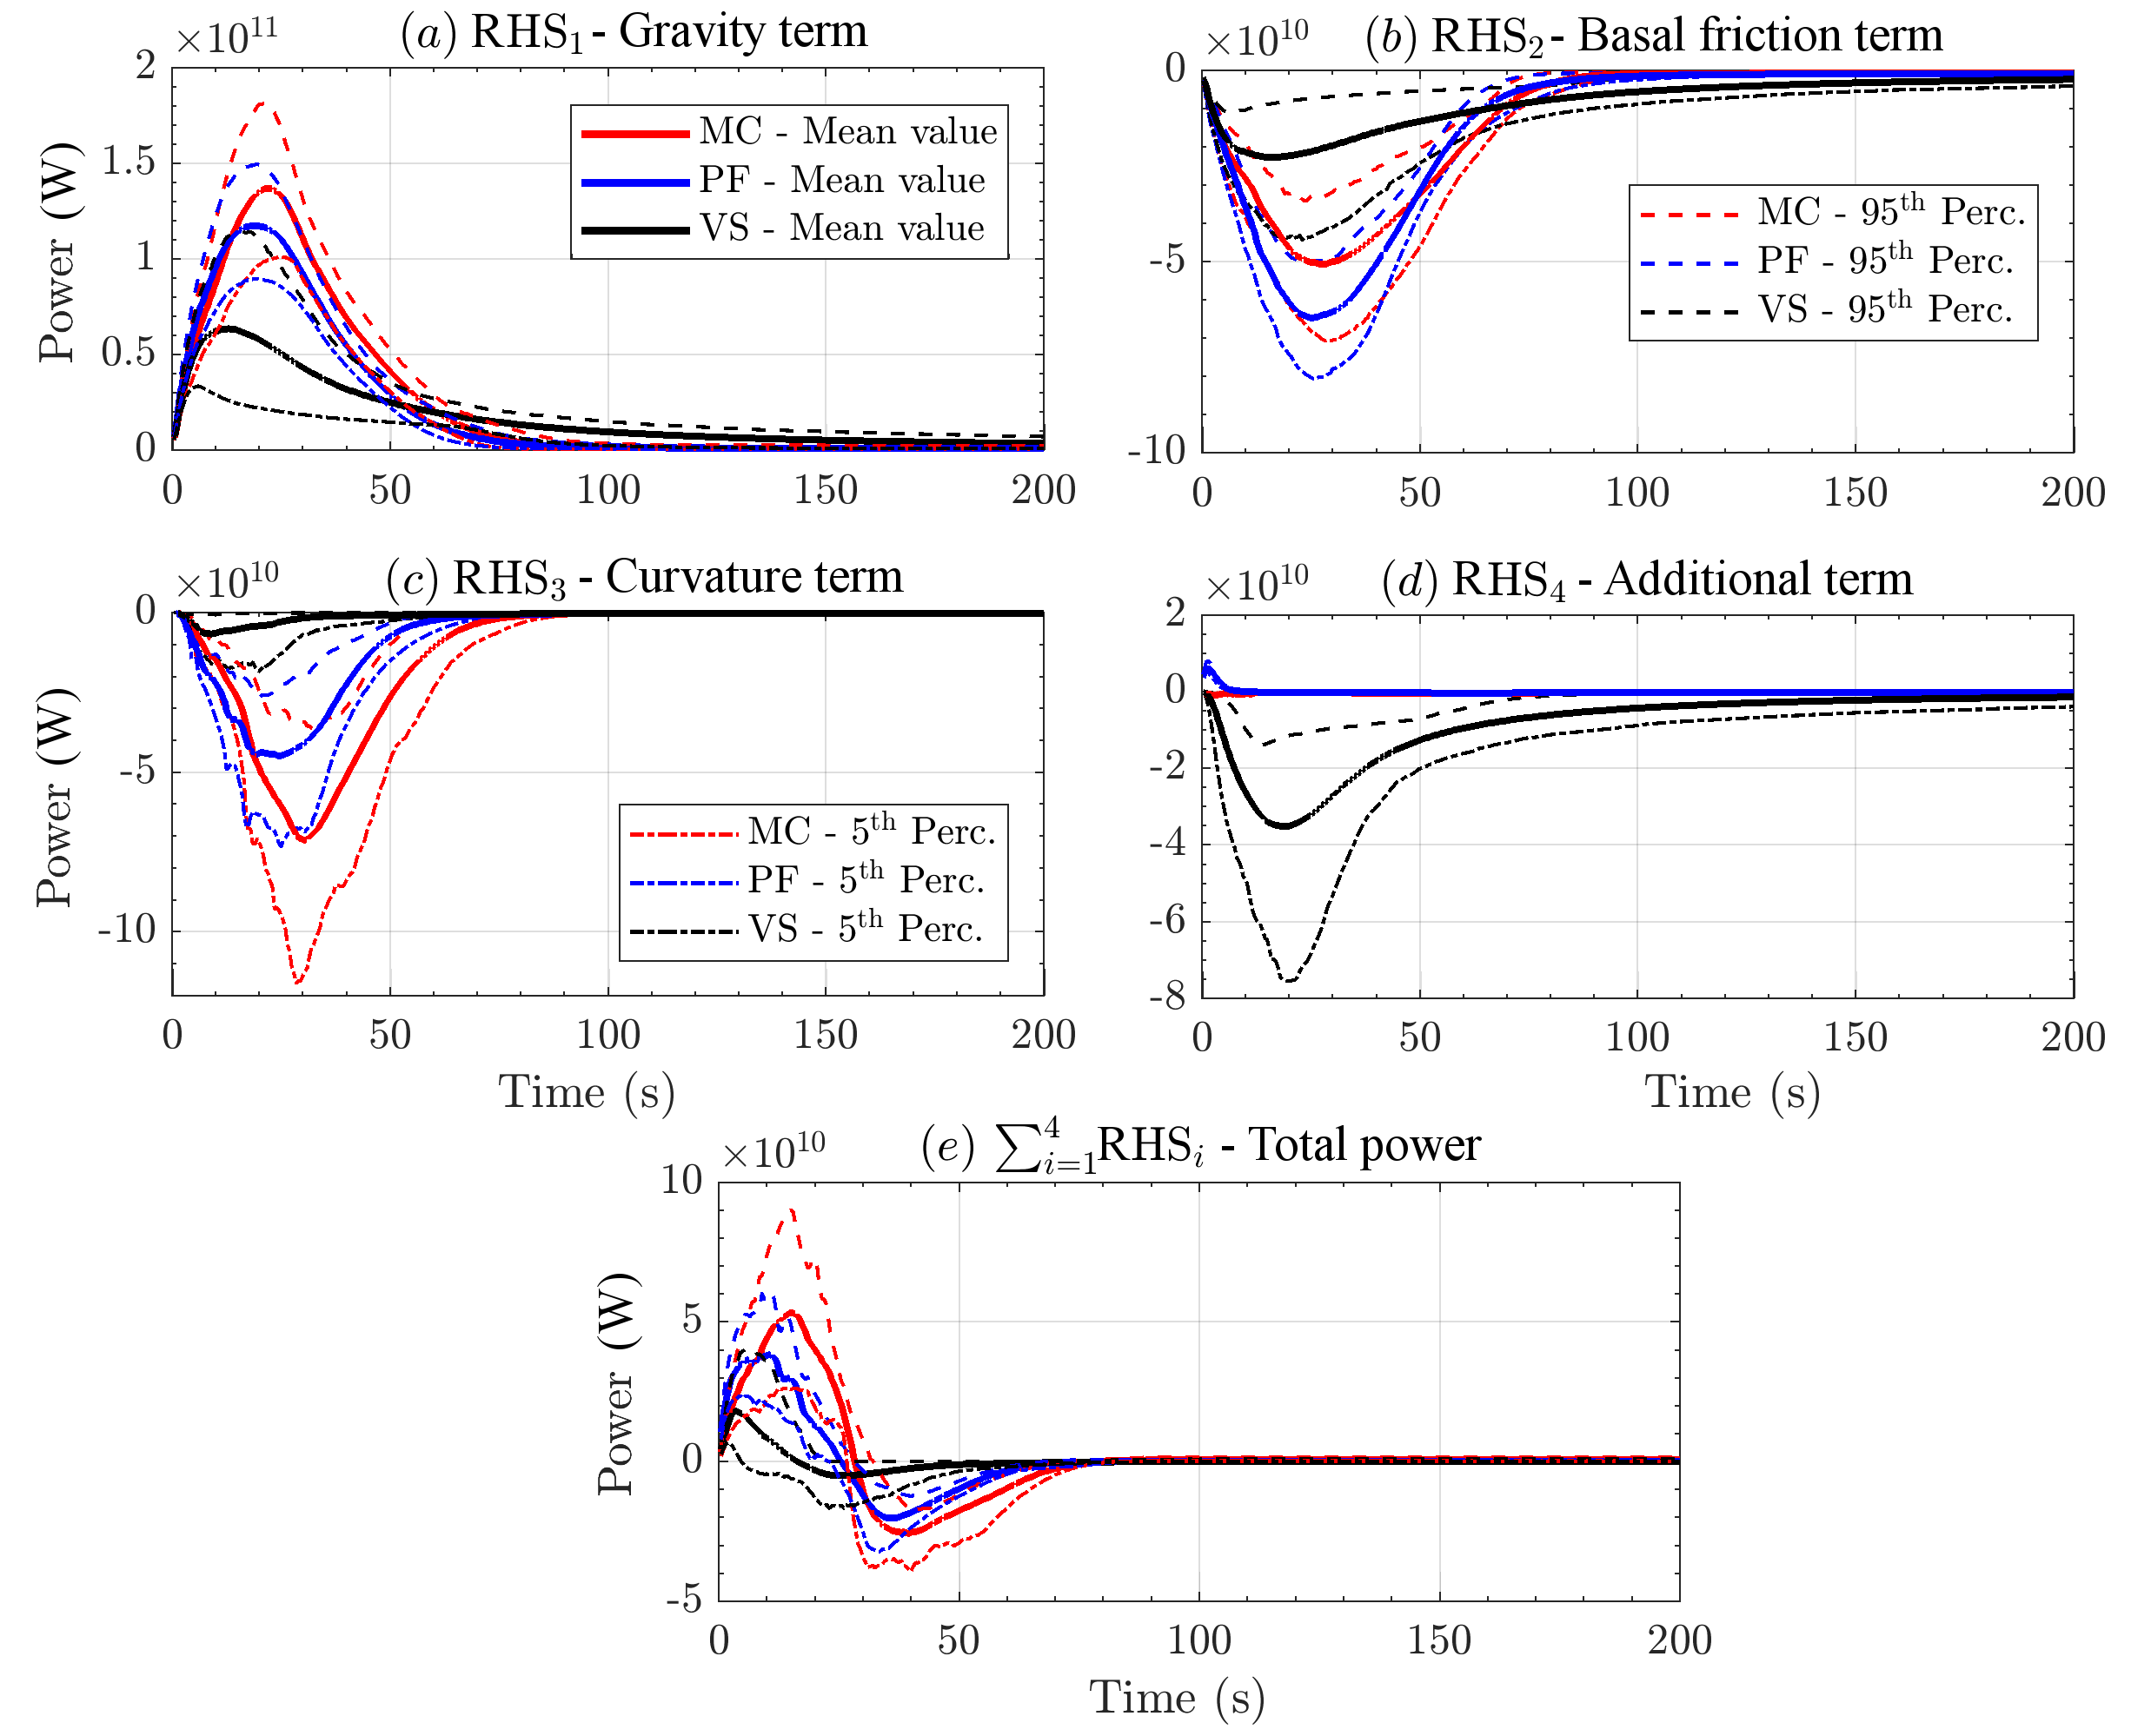
\includegraphics[width=0.95\textwidth]{BAF_VolcanDeColima/AveragedMeasurments/PowersColima.png}
        \caption{Spatial integrals of the RHS powers. Bold line is mean value, dashed lines are 5$^{\mathrm{th}}$ and 95$^{\mathrm{th}}$ percentile bounds. Model comparison on the mean value is also displayed. Different models are displayed with different colors.}
        \label{fig:Colima-Power-spatial}
\end{figure}
The scalar product of force with velocity imposes the bell-shaped profile already observed in Fig. \ref{fig:Ramp-Power-spatial}a. In plot \ref{fig:Colima-Power-spatial}a the power of $\boldsymbol{RHS_1}$ represents the effect of the gravity. It starts from zero and rises up to $\sim 1.4e11 W$ in MC, $\sim 1.2e11 W$ in PF, $\sim 6.5e10 W$ in VS. Uncertainty is $\pm 4e10 W$ in MC, $\pm 3e10 W$ in PF, $[-4e10,+5e10] W$ in VS. The decrease of gravitational power is related to the slope reduction, and this decrease is more gradual in VS than in the other models. In plot \ref{fig:Colima-Power-spatial}b the power of  $\boldsymbol{RHS_2}$ represents the effect of the basal friction in all the models. It is negative and peaks to $\sim -6.5e10 W$ in MC, $\sim -5e10 W$ in PF, $\sim -2e10 W$ in VS. In VS this dissipative power is significantly more flat than in the other models. MC and PF show negligible powers after $\sim 100 s$, VS after $\sim 200 s$. Uncertainty is $\pm 2e10 W$ in MC, $\pm 1.5e10 W$ in PF, $[-2e10,+1e10] W$ in VS. In PF, the plot starts from stronger values than in the other models, but it is also the faster to wane. In plot \ref{fig:Colima-Power-spatial}c the power of $\boldsymbol{RHS_3}$ represents the effect of the curvature of terrain. It has a negative peak at $\sim -7e10 W$ in MC, $\sim -4.5e10 W$ in PF, $\sim -5e9 W$ in VS. Uncertainty on the peak value is $[-4.5e10,+3.5e10] W$ in MC, $[-2.5e10,+2e10] W$ in PF, $[-1e10,+5e9] W$ in VS. The three models all show a bell-shaped profile, MC and PF waning to zero at $90 s$, VS at $\sim 30 s$. In plot \ref{fig:Colima-Power-spatial}d the power of $\boldsymbol{RHS_4}$ has a different meaning in the three models. In MC it is the internal friction term, and it only has almost negligible ripple visible in the first second. In PF it is a depth averaged correction in the hydrostatic pressure, and has an almost negligible effect only during the first second of simulation, at $5e9 W$. It becomes null at $\sim 10 s$. In VS, instead, it is a speed dependent term, and has a very relevant effect. The plot shows a bell-shaped profile, with a peak of $\sim -3.5e10 W$, $[-2e10,+1e10] W$. After that, this dissipative power gradually decreases, and becomes negligible at $200 s$.

\section{Discussion on the comparative anatomy of geophysical flow models}
In this section we summarize the general features which differ between the models. The mean plots are significantly informative, and the uncertainty ranges often exalt the differences between the models. After this, we describe a new method for statistically evaluating the performance of the couple $\left(M, P_M\right)$ according to a specific observation.

\subsection{Characteristic features and their motivations}
The different features in the models macroscopically affect the shape of the inundated area, both in the small flow on the inclined plane, and in the large scale geophysical flow. In Fig. \ref{fig:Ramp-first}b the flow runout displays a larger lateral extent in PF, and a bent shape in VS - the lateral wings remain behind the central section of the flow. Also in Fig. \ref{Colima-MaxMinExtents}, the three models look clearly different. Even if the maximum runout is matched between the models, MC displays a further distal spread before entering the ravines, PF shows a larger angle of lateral spread at the initiation pile, VS is less laterally extended and generally looks significantly channelized, and displays several not-inundated spots due to minor topographical coul\'{e}es.

\subsubsection{Flow height and acceleration}
Flow height gives additional insight on the model features. In Fig. \ref{fig:Ramp-H}, MC is more distally stretched, but starts to deposit material earlier and closer to the initial pile compared to the other models. PF height is generally shorter, and displays a small temporal anticipation in its arrival at the sample points. These features are probably due to the hydrostatic correction term, which additionally pushes forward the material during the pile collapse. A linear cut in the flow height profile of PF is also observed when the flow thins on the slope. That is probably generated by the interpolation between the two basal friction angles as a function of flow height and speed. VS tends to be higher than the other models, if observed at the same instant, because of the reduced lateral spreading of material.

In Fig. \ref{fig:Colima-H} the flow height plots allow us to classify the local flow regimes according to their similarity with what observed in the four sample points of the small scale case study. There is a new feature which was not present in the small scale flow - VS is temporally stretched, and material arrives later and stays longer in all the sample points. This is clearly a consequence of the speed dependent term reducing flow velocity.

Flow acceleration brings our analysis from the mechanics to the dynamics of the flow. In Fig. \ref{fig:Ramp-AccL}, at the point on the slope, MC has a flat plateau, while PF is linearly decreasing, and VS is bell shaped. Those differences are a consequence of the assumptions behind the models - double bed friction angle in PF, and speed dependent term in VS. At the slope change point, VS and MC display a bimodal profile in the acceleration. This is not a statistical effect, but it is also observed in single simulations. The first maximum is when the head of the flow hits the ground, while the second maximum is when the accumulating material in the tail arrives there. In VS the maxima are equal, because the tail is not laterally spread and hits the ground compactly. In contrast, PF does not show such a second peak, due to the accentuated lateral spreading in the tail. On the flat runway, the average acceleration in PF is lower than in the other models, probably because the material stops more suddenly.

\subsubsection{Statistical analysis of latent variables}
The dominance factors illustrate the predominant force term through time. In Fig. \ref{fig:Ramp-Pr_x} the differences between the models are minor in the inclined plane case study. In general, there is always a single dominant force, and its profile is complementary with the no-flow probability. In the slope change point the differences between the models are more significant. Curvature term dominance probability is bimodal in MC and VS, and in VS the two peaks are equivalent. On the flat runway, in PF the hydrostatic correction can be the dominant force with a small chance. In Fig. \ref{fig:Ramp-Ci_x} the contribution coefficients illustrate the relative scale of all the forces, and show that the second strongest force is never above 60\% of the dominant.

In Fig. \ref{fig:Colima-Pr1} and \ref{fig:Colima-Pr2}, the complexity in the dominance factors is remarkable. In the proximal points to the initiation, gravitational force is dominant with a high probability until the no-flow probability become predominant. In MC and PF curvature force can be dominant for a short time. In VS gravitational force is dominant for a larger time span than in the other models, because of the longer presence of the flow. Also the speed dependent friction can be dominant with a small probability at the beginning of the dynamics, when the flow is faster.

In most of the distal points, the basal friction is dominant with high probability. Some of the points have a deposit at the end with a high chance, some other not, depending on the slope. In general, in MC the no-flow probability tends to be larger than in the other models, because some flow samples stops earlier, or completely leaves the site. Again, curvature can have a small chance to be dominant in MC and PF, particularly when the speed is high.

Point $L_{43}$ is particularly interesting. It is not proximal to the initiation and it is placed right after a local hill. This location shows an intermediate regime between the proximal points and the distal ones. The no-flow probability is increasing at the end, meaning that the material is still leaving the site. Moreover, the gravity can be dominant like in the proximal points, but also the bed friction can be dominant. In MC and VS both the two forces have similar chances to be dominant for the most of the time of the simulation. In PF, only the gravitational force is dominant with a high chance, and the no-flow probability is almost null, meaning that there is accelerating material for the most of time. This is probably because point $L_{43}$ is situated downhill of a place where a significant amount of material stops according to that model.

\subsubsection{Flow extent and spatial integrals}
In Fig. \ref{fig:Ramp-spatial} the spatially averaged speed and Froude Number are significantly similar between the models. The differing features appear to be mostly localized in space. However, VS is confirmed to be significantly slower than the other models after the initial collapse. Moreover, it is the only model which presents a significant amount of long lasting and slowly moving material. Inundated area in PF has a greater maximum value, because of the accentuated lateral spread. In VS the inundated area almost does not decrease from its peak, because of the strictly increasing lateral spread. Vice versa, lateral spread in MC and PF has a temporary stop when the bulk of the flow hits the ground. This is a consequence of the interplay of accumulating material and the push of new material, which is stronger in the middle than in the lateral wings. In PF lateral extent weakly decreases for a short time. The hydrostatic correction term may generate the pull reducing the lateral extent. In Fig. \ref{fig:Colima-spatial} average speed and Froude Number display that VS slower speed is not a local feature. Inundated area is again significantly larger in PF than in the other models.

Spatial integrals of power terms have several features in common with the corresponding forces, and provide a decomposition of the acceleration sources. Main dissimilarity between forces and powers is that gravitational and basal friction powers have a profile starting from zero when the flow initiates, because the flow speed starts from zero. In Fig. \ref{fig:Ramp-Power-spatial} the differences between models are particularly relevant in term  $\boldsymbol{RHS_4}$. Speed dependent power in VS is at least one order of magnitude larger than the maximum values of the corresponding terms in MC and PF. Those are decreasing to zero after a short time from the initiation. Hydrostatic correction in PF is clearly positive in the speed direction, and hence contributing to push the flow ahead. The effects of internal friction in MC are almost negligible, and initially positive, then negative. This is motivated by an initial compression of the material during the pile collapse, followed by its stretching. It is worth remarking that $\boldsymbol{RHS_2}$ and $\boldsymbol{RHS_3}$ are both smaller in VS, due to the lower basal friction angles involved. In Fig. \ref{fig:Colima-Power-spatial}, the differences are accentuated, because of the topography complexity. Gravity term is larger in VS, because a portion of the flow lingers on the higher slopes for a long time. Basal friction has a higher peak in PF compared to the other models, due to the interpolation of the two basal friction angles.

\subsection{Example of model performance calculation}
Analysis of model suitability can be conducted. In past work \cite{Patra2005}, MC rheology was tuned to match deposits for known block and ash flows, but {\it a priori} predictive ability was limited by inability to tune without knowledge of flow character. The new procedure developed in this study enables the quantification of model performance, i.e. the similarity of the outputs and real data. We remark that the measured performance refers to the couple $\left(M, P_M\right)$, and that different parameter ranges can produce different performances. Our example concerns the Volc{\'a}n de Colima case study, and in particular we compare the inundated region in our simulations to the deposit of a BAF occurred 16 April 1991 \citep{Saucedo2004, Rupp2004, Rupp2006}. The inundated region is defined as the points in which the maximum flow height $H$ is greater than $10 cm$. A similar procedure may be applied to any observable variable produced by the models, if specific data become available.

Let $\mathcal M:\mathcal P(\mathbb R^2)\rightarrow[0,1]$ be a similarity index defined on the subsets of the real plane. An equivalent definition can be based on the pseudo-metric $1-\mathcal M$. For example, we define
$$\mathcal M_I:=\frac{\int_{\mathbb R^2} 1_{S \cap D}(\textbf{x}) d\textbf{x}}{\int_{\mathbb R^2} 1_D(\textbf{x})d\textbf{x}},\quad \mathcal M_U:=\frac{\int_{\mathbb R^2} 1_D(\textbf{x})d\textbf{x}}{\int_{\mathbb R^2} 1_{S \cup D}(\textbf{x}) d\textbf{x}}, \quad \mathcal J:=\mathcal M_I\cdot \mathcal M_U,$$
where $S\subset \mathbb R^2$ is the inundated region, and $D\subset \mathbb R^2$ is the recorded deposit. In particular, $\mathcal M_I$ is the area of the intersection of inundated region and deposit over the area of the deposit, $\mathcal M_U$ is the area of the deposit over the area of the union of inundated region and deposit, $\mathcal J$ is the product of the previous, also called Jaccard Index \citep{Jaccard1901}.

Figure \ref{fig:Colima-Hist} shows the probability distribution of the similarity indices, according to the uniform probability $P_M$ on the parameter ranges defined in this study. Different metrics can produce different performance estimates, for example MC inundates most of the deposit, but overestimates the inundated region, while VS relatively reduces the inundated region outside of the deposit boundary, but also leaves several not-inundated spots inside it.

Let $g:[a,b]\rightarrow[0,1]$ be a score function defined over the percentile range of the similarity index. The global $5^{th}$ and $95^{th}$ percentile values $[a,b]$ are defined assuming to select the model randomly with equal chance, and are also shown in Fig.\ref{fig:Colima-Hist}a,b,c. Then the performance score $G_g$ of model $\left(M, P_M\right)$ is defined as:
$$G_g\left(M, P_M\right)=\int_{[a,b]} g(x) df_M(x),$$
where $f_M$ is the pdf related to the model. Possible score functions include a step function at the global median, a linear or quadratic function, a sigmoid function. Supporting Information S8 reports a Table of alternative performance scores, according to changing similarity indices and score functions.

\begin{figure}[H]
         \centering
        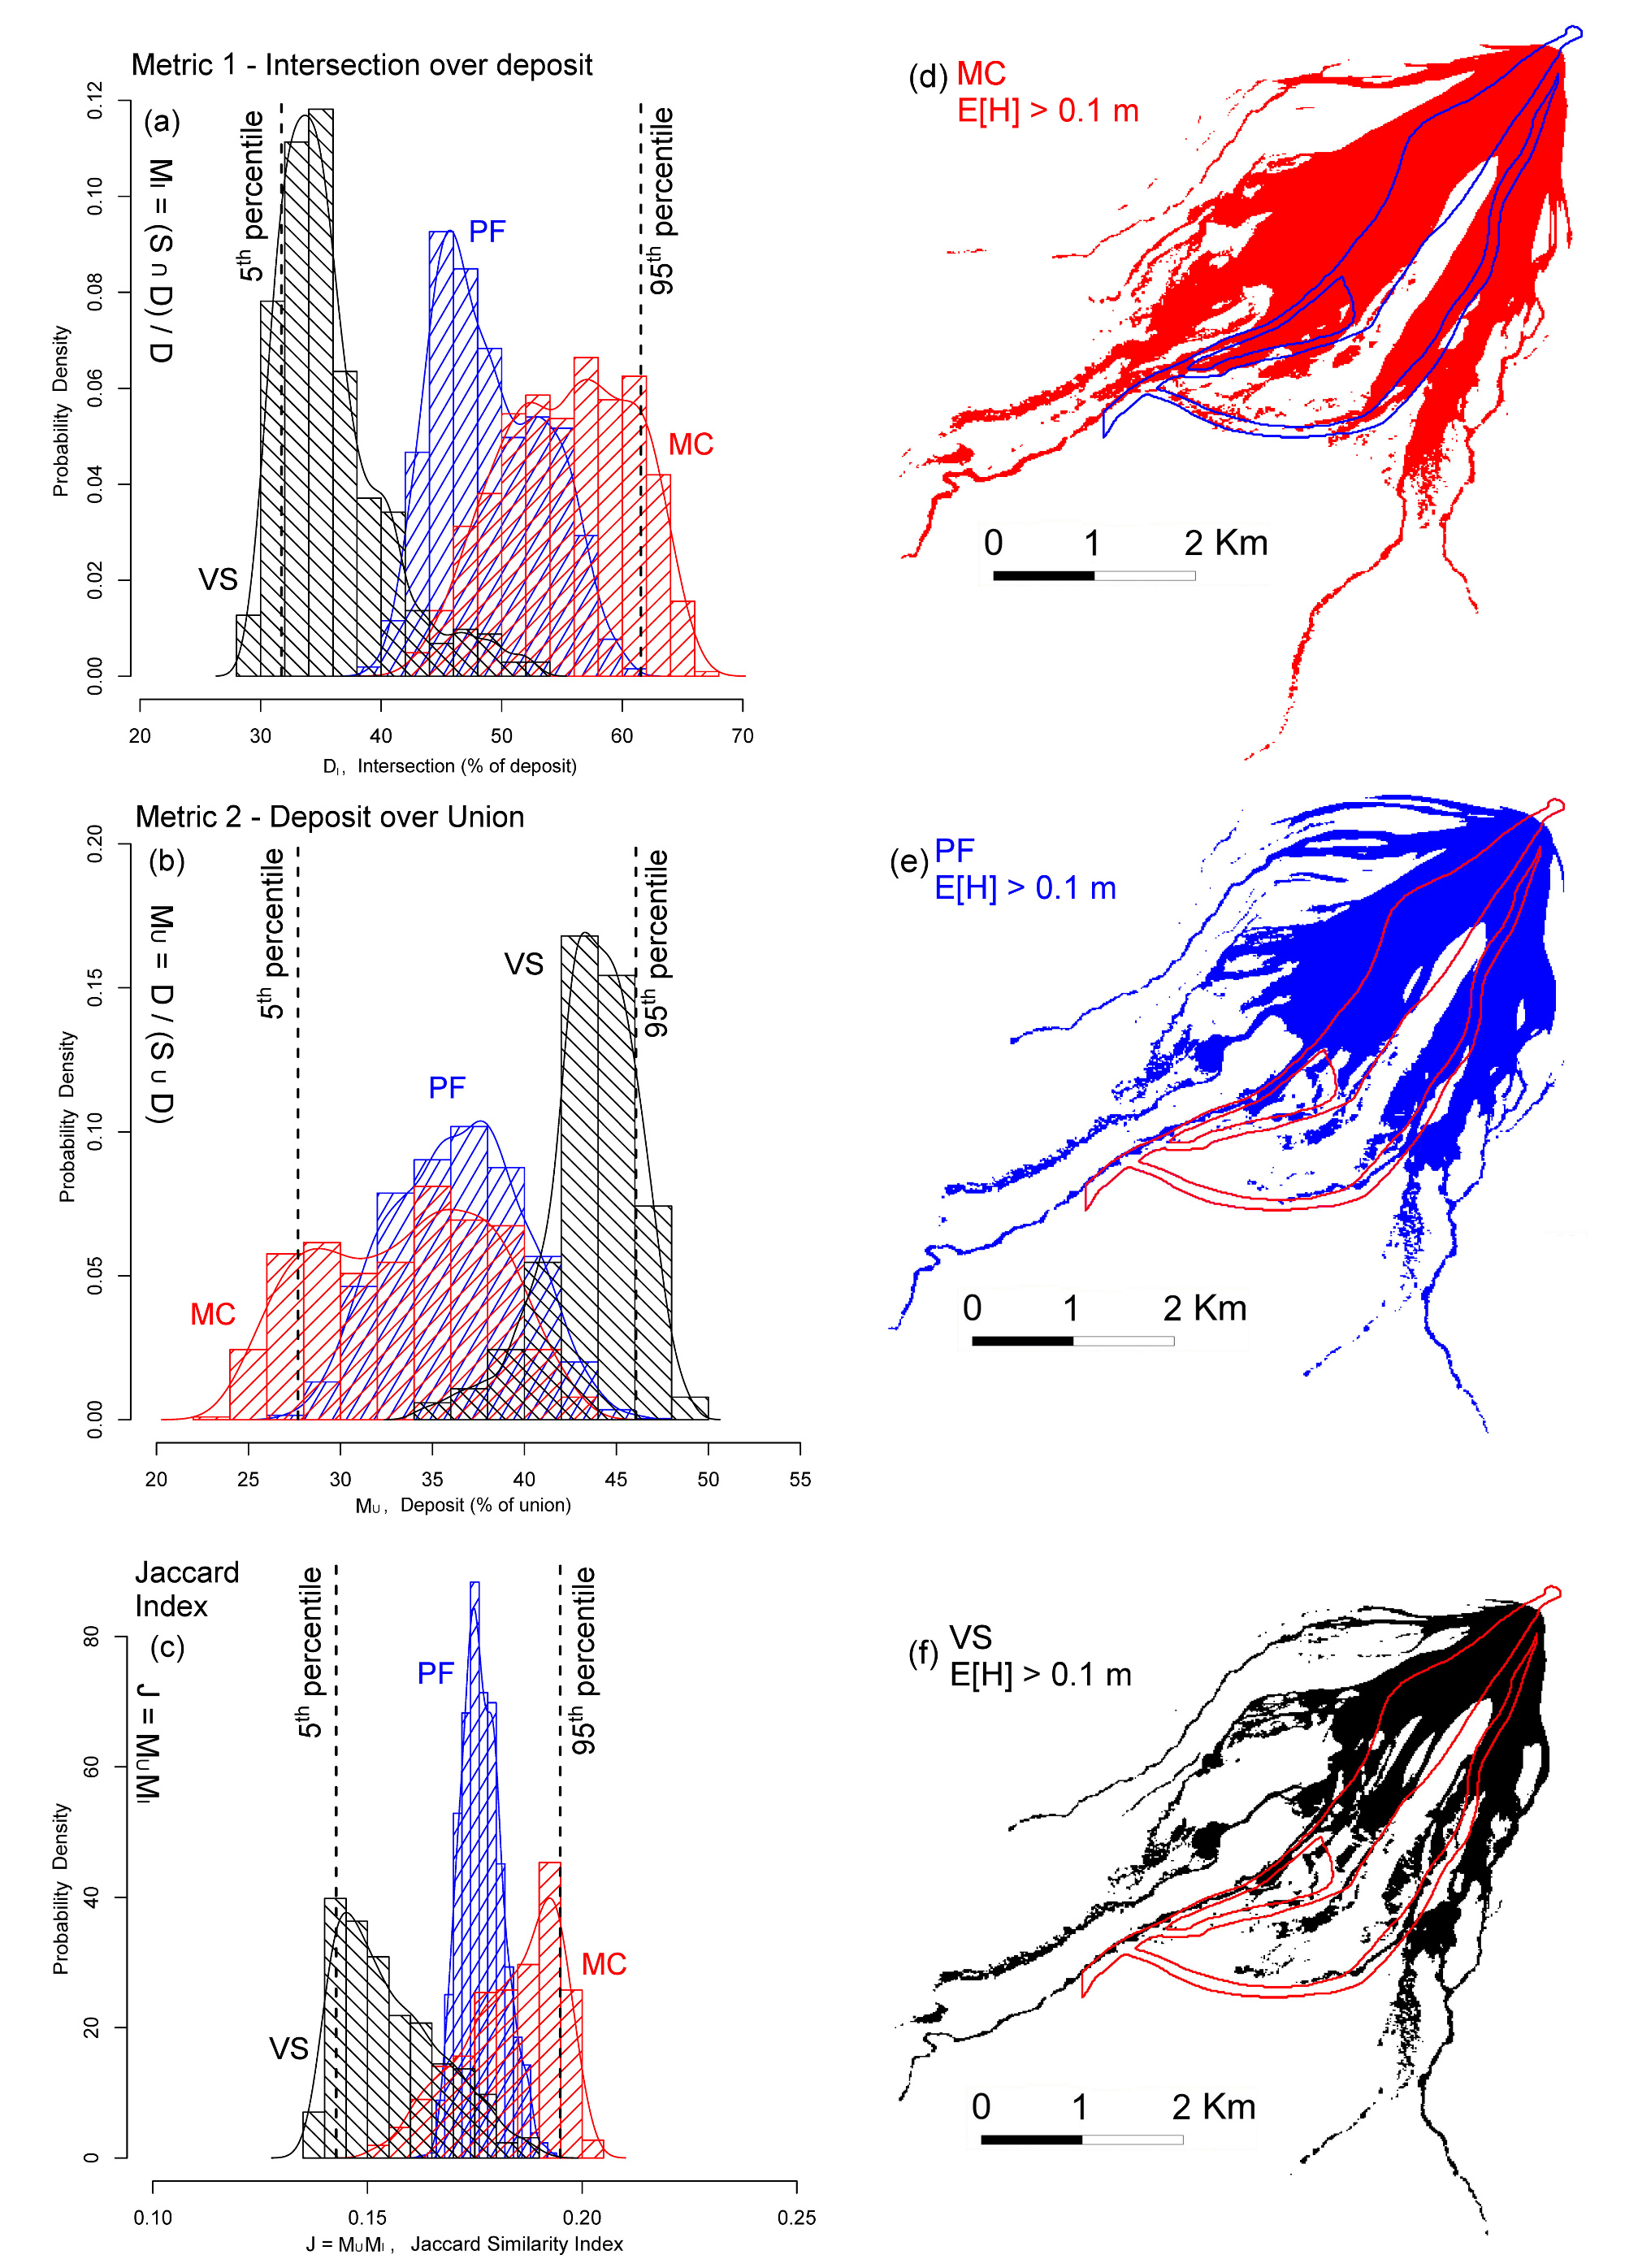
\includegraphics[width=0.82\textwidth]{Figures/Histograms.jpg}
        \caption{Probability density functions of the similarity indices of the Volc{\'a}n de Colima inundated regions with the deposit of the 16 April 1991 BAF. (a) is based on $\mathcal M_I$, (b) on $\mathcal M_U$, (c) on $\mathcal J$. Different colors correspond with the models MC (red), PF (blue), VS (black). Data histograms are displayed in the background. Global $5^{th}$ and $95^{th}$ percentile values are indicated with dashed lines. Plots (d,e,f) display the average inundated region $\left\{\textbf{x} : E[H(\textbf{x}]>10 cm\right\}$. The boundary of the real deposit is marked with a colored line.}\label{fig:Colima-Hist}
\end{figure}

\section{Conclusions}
In this study, we have introduced a new statistically driven method for analyzing complex models. We have used three different models arising from different rheology assumptions. The data shows unambiguously the performance of the models across a wide range of possible flow regimes and topographies. The analysis of latent variables is particularly illustrative of the impact of modeling assumptions. Knowledge of which assumptions dominate, and, by how much, will allow us to construct efficient models for desired inputs. Such model composition is the subject of ongoing and future work, with the purpose to bypass the search for a unique best model, and yet to go beyond a simple mixture of alternative models.

In summary, our new method enabled us to break down the effects of the different physical assumptions in the dynamics, providing an improved understanding of what characterizes each model. The procedure was applied to two different case studies: a small scale inclined plane with a flat runway, and a large scale DEM on the SW lope of Volc\'{a}n de Colima (MX). In particular, we presented:
\begin{itemize}
  \item a short review of the assumptions characterizing three commonly used rheologies of Mohr-Coulomb, Poliquenne-Forterre, Voellmy-Salm. This included a qualitative list of such assumptions, and a breaking down of the different terms in their differential equations.
  \item an new statistical framework, processing the mean and the uncertainty range of either observable or latent variables in the simulation. The new concept of force dominance factors enabled a simplified description of the local dynamics. These quantities were analyzed at selected sites, but spatial integrals were also performed, illustrating the characteristics of the entire flow.
  \item a final discussion, explaining all the observed features in the results on the light of the known physical assumptions of the models, and the evolving flow regime in space and time. This included a new model performance estimation method, depending on the metric and the cost function adopted.
\end{itemize}

Our statistical analysis based on UQ depicted the following main features:
\begin{itemize}
  \item Compared to a classical MC model, PF lacks of internal friction and this produces an accentuated lateral spread. This is increased by the hydrostatic correction, which briefly pushes the flow ahead and laterally during the initial collapse. That force can also have some minor effects in the final deposit accumulation. The interpolation of the smaller bed friction angle $\phi_1$ with the larger value $\phi_2$, suddenly stops the flow if it thins compared to its speed. This mechanism does not allow for large speed peaks.
  \item Instead in VS, the speed dependent friction has a great effect in reducing lateral spread and producing channeling features even due to minor ridges in topography. The flow tends to be significantly slower and more stretched in the slope direction. The effects of the different formulation of the curvature term are less impacting than the effects of the lower basal friction and speed.
\end{itemize}

Additional research concerning other case studies, and different parameter ranges, might reveal other flow regimes, and hence differences in the consequences of the modeling assumptions under new circumstances.


\section{Appendix A: Latin Hypercubes and orthogonal arrays}
The Latin Hypercube Sampling (LHS) is a well established procedure for defining pseudo-random designs of samples in $\mathbb R^d$, with good properties with respect to the uniform probability distribution on an hypercube $[0,1]^d$ \citep{McKay1979,Owen1992b,Stein1987,Ranjan2014,Mingyao2016}. In particular, compared to a random sampling, a LHS: (i) enhances the capability to fill the d-dimensional space with a finite number of points, (ii) in case $d>1$, avoids the overlapping of point locations in the one dimensional projections, (iii) reduces the dependence of the number of points necessary on the dimensionality $d$.

\begin{definition}[Latin hypercube sampling]
Let $\Xi=\{\xi_i\ :\ i=1,\dots,N\}$ be a set of points inside the d-dimensional hypercube $C=[0,1]^d$. Let $[0,1]=\bigcup_{j=1}^{N} I_j$, where $I_j=[\frac{(j-1)}{N},\frac{j}{N}]$. Let $\xi_i=\left(\xi_i^1,\dots,\xi_i^d\right)$, and for each $k\in\{1,\dots,d\}$, let $\Xi^k=\{\xi^k_i\ :\ i=1,\dots,N\}$. Let $\lambda^d$ be the uniform probability measure supported inside $C$, called Lebesgue measure. Then $\Xi$ is a latin hypercube w.r.t. $\lambda^d$ $\Longleftrightarrow$ $\forall j\in \{1,\dots,N\}$, $\forall k\in\{1,\dots,d\}$, $\left|I_j\cap\Xi^k\right|=1$.
\end{definition}

The procedure is simple: once the desired number of samples $N\in\mathbb N$ is selected, and $[0,1]$ is divided in $N$ equal bins, then each bin will contain one and only one projection of the samples over every coordinate. The LHS definition is trivially generalized over $C=\prod^d_i [a_i, b_i]$, i.e. the cartesian product of $d$ arbitrary intervals. That will be applied in this study, defining LHS over the parameter domain of the flow models.

There are a large number of possible designs, corresponding the number of permutations of the bins in the d-projections, i.e. $d\cdot N!$. If the permutations are randomly sampled there is a high possibility that the design will have good properties. However, this is not assured, and clusters o points or regions of void space may be observed in $C$. For this reason, we base our design on the orthogonal arrays (OA) \citep{Owen1992a,Tang1993}.

\begin{definition}[Orthogonal arrays]
Let $S=\{1,\dots,s\}$, where $s\ge 2$. Let $Q\in S^{n\times m}$ be a matrix of such integer values. Then $Q$ is called an $OA(n,m,s,r)$ $\Longleftrightarrow$ each $n\times r$ submatrix of $Q$ contains all possible $1\times r$ row vectors with the same frequency $\lambda=n/s^r$, which is called the index of the array. In particular, $r$ is called the strength, $n$ the size, $(m\ge r)$ the constrains, and $s$ the levels of the array.
\end{definition}

Orthogonal arrays are very useful for defining latin hypercubes which are also forced to fill the space (or its r-dimensional subspaces) in a more robust way, at the cost of potentially requiring a larger number of points than a traditional LHS.

\begin{proposition}
Let $Q$ be an $OA(n,m,s,r)$. Then let $U\in\mathbb R^{n\times m}$ be defined as follows:
$$\forall k\in \{1,\dots,s\},\ \forall j\in \{1,\dots,m\},\ \left\{Q[\cdot,j]\ :\ Q[i,j]=k\right\} = \Pi\left(\{(k-1)\lambda s^{r-1},\dots, k\lambda s^{r-1}\}\right),$$
where $\Pi$ is a random permutation of $\lambda s^{r-1}$ elements. Then $\Xi=\{\xi_i=U[i,\cdot]\ :\ i=1,\dots,n\}$ is a LHS w.r.t to $\lambda^m$ over $C=[0,1]^m$. Moreover, let $[0,1]^r=\bigcup_{(h_1,\dots,h_r)=1}^{s} I_{(h_i)}$, where $I_{(h_i)}=\prod^r_i[\frac{(h_i-1)}{s},\frac{h_i}{s}]$. Then $\forall D=(d_1,\dots,d_r)\subseteq \{1,\dots,m\}$, let $\Xi^D=\{(\xi^{d_1},\dots,\xi^{d_r})\ :\ i=1,\dots,n\}$. We have that
$$\forall k\in \{1,\dots,s\},\ \forall (h_i\ : i=1,\dots,r)\in\{1,\dots,d\}^r,\ \left|I_{(k_i)}\cap\Xi^D\right|=\lambda.$$
\end{proposition}

For each column of $Q$ we are replacing the $\lambda s^{r-1}$ elements with entry $k$ by a random permutation of $\left((k-1)\lambda s^{r-1} + h\right)_{h\in 1,\dots, \lambda s^{r-1}}$. After the replacement procedure is done, the newly obtained matrix $U$ is equivalent to a LHS which inherits from $Q$ the property of fully covering $s^r$ equal r-dimensional hypercubes in every r-dimensional projection. Each hypercube contains $\lambda$ points. In other words, inside each r-dimensional projection, the design associated to $U$ fills the space like a regular grid at the scale of those $s^r$ hypercubes, but it is still an LHS at a finer scale, i.e. the $\lambda s^{r-1}$ one dimensional bins. A complete proof can be found in \cite{Tang1993} and it is a straightforward verification of the required properties.

However, even in an LHS based on an $OA(n,m,s,r)$, if $r<m$ what happens in the projections with dimension $r'>r$ is not controlled, and randomizing procedures are made more difficult by the additional structure imposed by the $OA$. Moreover, the total number of points necessary to achieve a full design increases with $r$, and hence is affected by dimensionality issues.

Dealing with relatively small $d$, i.e. $d\in\{3,4\}$, we adopt a LHS $U$ created by a $OA(s^d,d,s,d)$. The strength is equal to the dimension $d$, hence the design fills the entire space like a $d$ dimensional grid, but it is a LHS as well. In this case there is one point in each hypercube, and $\lambda=1$. We take $s=8$ for the 3-dimensional designs over the parameter space of Mohr-Coulomb and Voellmy-Salm models, i.e. $512$ points; we took $s=6$ for the 4-dimensional designs over the more complex parameter space of the Pouliquen-Forterre model, i.e. 1296 points.

\section{Appendix B: Force contribution coefficients, and their conditional decomposition}
There is an additional result explaining the meaning of those coefficients through the conditional expectation.
\begin{proposition}
Let $(F_i)_{i\in I}$ be random variables on $(\Omega, \mathcal F, P)$, representing the considered force components in location $x$ at time $t$. For each $i$, let $C_i$ be the contribution coefficient of force $F_i$, assuming $\Phi=\Phi_2$. Then we have the following expression:
$$C_i=\sum_j p_j \mathbb E\left[\frac{F_i}{|F_j|}\ \Big{|}\ \Phi=|F_j|\right],$$
where $p_j:=P\left\{\Phi=|F_j|\right\}$.
\end{proposition}

\begin{proof}
Let $Z$ be a discrete random variable such that, for each $j\in\mathbb N$, $(Z=j) \Longleftrightarrow (\Phi=|F_j|)$. Then, by the rule of chain expectation:
$$C_i=\mathbb E\left[\frac{F_i}{\Phi}\right]=\mathbb E\left[\mathbb E\left[\frac{F_i}{\Phi}\ \Big{|}\ Z=j\right]\right]=$$
$$=\mathbb E\left[\mathbb E\left[\frac{F_i}{|F_j|}\ \Big{|}\ Z=j\right]\right]=\sum_j P\left\{Z=j\right\} \mathbb E\left[\frac{F_i}{|F_j|}\ \Big{|}\ Z=j\right].$$
Moreover, by definition, $p_j=P\left\{Z=j\right\}$. This completes the proof.
\end{proof}

The last proposition brings to a conditional decomposition of the contribution coefficients, taking advantage of the \emph{dominance factors} $(p_j)_{j=1,\dots, k}$, i.e. the probability of each $F_j$ to be the dominant force in $(x,t)$.

\begin{definition}[Conditional contributions and dominance factors]
Let $(F_i)_{i=1,\dots, k}$ be random variables on $(\Omega, \mathcal F, P)$, representing arbitrary force components in location $x$ at time $t$. Then, for each pair of components $(i,j)$, the conditional contribution $C_{i,j}$ is defined as:
$$C_{i,j}:=\mathbb E\left[\frac{F_i}{|F_j|}\ \Big{|}\ \Phi=|F_j|\right],$$
where $\Phi=\Phi_2$ is the dominant force. In particular, for each component $i$, the dominance factor is defined as:
$$p_j:=P\left\{\Phi=|F_j|\right\}.$$
\end{definition}

\newpage
\bibliographystyle{apalike}
\bibliography{mybibfile}

\end{document}
